\documentclass[a4paper, 12pt, BCOR10mm, DIV12, toc=bibliography, toc=listof, german]{scrbook}

% Preamble {{{
\usepackage[ngerman]{babel}
\usepackage[utf8]{inputenc}
\usepackage[T1]{fontenc}
\usepackage[pdftex]{graphicx}
\usepackage[%
	colorlinks=false,
	pdfborder={0 0 0},
]{hyperref}
\usepackage{epstopdf}
\usepackage[numbers,sort]{natbib}
\usepackage{setspace}
\usepackage{amsmath, amsthm, amssymb}
\usepackage{scrpage2}
\usepackage{units}
\usepackage{listings}
\usepackage{color}
\usepackage{xcolor}

\definecolor{uniblue}{rgb}{0.062745,0.17647,0.34118}
\definecolor{tblue}{HTML}{729FCF}
\definecolor{tgreen}{HTML}{8AE234}
\definecolor{tred}{HTML}{EF2929}

\lstset{
	language=C,
	numbers=left,
	frame=single,
	basicstyle=\footnotesize,
	showstringspaces=false,
	captionpos=b,
	breaklines=true,
	breakatwhitespace=false,
	keywordstyle=\color{tgreen},
	commentstyle=\color{tblue},
	stringstyle=\color{tred}
}

\setcounter{secnumdepth}{3}
\setcounter{tocdepth}{3}

\def \dns {Domain Name System (DNS)}

% Titlepage {{{
\usepackage[absolute]{textpos}

\newlength{\TitleMargin}
\newlength{\TitleWidth}

\setlength{\TitleMargin}{2cm}
\setlength{\TitleWidth}{\paperwidth}
\addtolength{\TitleWidth}{-\TitleMargin}
\addtolength{\TitleWidth}{-\TitleMargin}


\newcommand{\TitleUni}{Universität Potsdam}
\newcommand{\TitleInstitut}{Mathematisch-Naturwissenschaftliche Fakultät\\Institut für Informatik}
\newcommand{\TitleTitel}{Selbst-adaptive Lastverteilung für DNS-Cluster}
\newcommand{\TitleTyp}{Masterarbeit}
\newcommand{\TitleAutor}{Sebastian Menski}
\newcommand{\TitleBetreuerText}{Betreuer}
\newcommand{\TitleBetreuer}{Prof. Dr. Bettina Schnor\\ &M.Sc. Jörg Zinke}
\newcommand{\TitleAbschlussText}{zur Erlangung des akademischen Grades\\Master of Science\\in Informatik}
\newcommand{\TitleOrt}{Potsdam}
\newcommand{\TitleDatum}{7. Juli 2012}
\hypersetup{
	pdfauthor={Sebastian Menski},
	pdftitle={\TitleTitel},
}

\renewcommand{\maketitle}{
	\thispagestyle{empty}
	\begin{textblock*}{\TitleWidth}(\TitleMargin,\TitleMargin)
		~\hfill
\includegraphics[height=2.5cm]{images/uni-logo}\\[3mm]
		{\color{uniblue}\rule{\TitleWidth}{1mm}}\\[5mm]
		{
			\centering
			\sffamily\Large
			{\LARGE\TitleUni}\\[0.5\baselineskip]
			{\large\TitleInstitut}\\[5\baselineskip]
			{\Huge\TitleTitel}\\[3\baselineskip]

			{\TitleTyp}\\
			\TitleAbschlussText\\[3\baselineskip]

			\TitleAutor\\[3\baselineskip]
			\begin{tabular}{rl}
				\TitleBetreuerText: & \TitleBetreuer
			\end{tabular}\\[2\baselineskip]
			\TitleOrt, \TitleDatum\par
		}
	\end{textblock*}~\clearpage{}
	\thispagestyle{empty}
	\noindent\begin{minipage}[t]{\textwidth}
	\end{minipage}\par
	\vfill
	\noindent\begin{minipage}[b]{\textwidth}
		{\textbf{Menski,~Sebastian}\\\texttt{menski@uni-potsdam.de}\\\TitleTitel\\\TitleTyp,~Institut für Informatik\\\TitleUni,~Juli
		2012}
	\end{minipage}\clearpage{}
  \thispagestyle{empty}
	\mbox{}\vfill
	\subsection*{\centering Zusammenfassung}

	Diese Masterarbeit befasst sich mit der Lastverteilung von DNS-Anfragen. Im Mittelpunkt steht
	dabei die Erweiterung der selbst-adaptiven Lastverteilungslösung \textit{salbnet}. Dazu wird für das System
	eine neue Metrik für UDP-Pakete konzipiert. Infolgedessen wird die Umsetzbarkeit des entwickelten
	Konzepts überprüft. Auf der Basis dieser Ergebnisse wird für \textit{salbnet} eine UDP-Erweiterung
	implementiert. Grundlage der Erweiterung ist eine Auswertung der UDP-Receive-Queue. Bei
	abschließenden Messungen konnte gezeigt werden, dass die Erweiterung funktionstüchtig ist und
	\textit{salbnet} im DNS-Anwendungsfall einem Standardalgorithmus überlegen ist.

	\vfill\mbox{}\clearpage
}


% Titlepage }}}

% Authorship {{{
\newcommand{\makeauthorship}{
  \chapter*{Selbstständigkeitserklärung}
  \thispagestyle{empty}
  Hiermit erkläre ich, dass ich die vorliegende Arbeit selbstständig angefertigt, nicht anderweitig zu Prüfungszwecken vorgelegt und keine anderen als die angegebenen Hilfsmittel verwendet habe. Sämtliche wissentlich
 verwendeten Textausschnitte, Zitate oder Inhalte anderer Verfasser wurden ausdrücklich als solche gekennzeichnet.\\[2ex]
  \iflanguage{ngerman}{\TitleOrt, den \TitleDatum\\[6ex]}{\TitleOrt, \TitleDatum\\[6ex]}
  {\flushleft
  \newlength\us
  \settowidth{\us}{-\TitleAutor-}
  \begin{tabular}{p{\us}}\hline
  \centering\footnotesize \TitleAutor
  \end{tabular}}
}

% Authorship }}}

% Preamble }}}

\begin{document}
	 % Frontmatter {{{
	\frontmatter
	\maketitle{}
	\makeauthorship{}
	\tableofcontents{}
	% Frontmatter }}}

	% Mainmatter {{{
	\onehalfspacing{}
	\mainmatter
	\pagestyle{scrheadings}

	\chapter{Einleitung} % {{{
	\label{cha:einleitung}

		Das \dns{} \cite{rfc1034, rfc1035} ist eine fundamentale Komponente des heutigen Internets.  Es
		ermöglicht eine Abbildung von Domain-Namen auf sogenannte IP\footnote{Das Internet Protocol (IP)
			\cite{rfc791} ist eines der wichtigsten Netzwerkprotokolle der TCP/IP-Suite
			\cite{stevens1994}. Es dient der Vermittlung von Datenpaketen in einem Netzwerk, um dies zu
		ermöglichen, erhält jeder Netzwerkteilnehmer eine eindeutige IP-Adresse.}-Adressen. Ein
		Domain-Name ist eine Zeichenkette, welche sich Menschen leichter einprägen können im Gegensatz
		zu einer Zahlenfolge. Im Unterschied dazu arbeiten Computersysteme hingegen effizienter und
		schneller  mit Zahlen als mit Zeichenketten.  Infolgedessen ist oben genannte Abbildung eine
		wichtige Voraussetzung für die einfache und schnelle Nutzung eines Netzwerks, im Besonderen des
		Internets. Bei jedem Aufruf einer Website oder dem Verschicken einer E-Mail, bei dem der Nutzer
		einen Domain-Namen verwendet, wird eine Abfrage an einen Server im DNS gestellt. Die
		darauffolgende Antwort, ist die dem Domain-Name zugeordnete IP-Adresse. Diese wird anschließend
		vom Computersystem genutzt, um eine Verbindung zum Ziel aufzubauen. Bereits dieser Zusammenhang
		verdeutlicht die Wichtigkeit des DNS, da ohne dieses System jeder Nutzer eines Netzwerks die
		benötigten IP-Adressen selbst kennen müsste. Für ein kleines privates Netzwerk ist dies
		eventuell durchaus möglich, in Anbetracht der Größe des heutigen Internets jedoch kaum
		vorstellbar. Aus diesem Grund ist ein stabiles System mit schnellen Antwortzeiten unerlässlich.

		Die Informationen im DNS werden dezentral gespeichert. Sie werden in einer verteilten,
		baumartigen Struktur gespeichert (siehe Abbildung \ref{fig:tree}). Dabei können verschiedene
		Server, die einzelnen Knoten des Baums und die dazugehörigen Informationen verwalten. Diese
		Server werden im Folgenden DNS-Server oder Nameserver genannt und haben die Aufgabe, Fragen an
		das DNS zu beantworten. Aus der Struktur, des in Abbildung \ref{fig:tree} dargestellten Baums, ist
		zu erkennen, dass die kritischste Infrastruktur in den ersten beiden Ebenen des Baums existiert.
		Dabei handelt es sich um den Root-Server und alle Server der Top-Level-Domains (TLDs). Diese
		beiden Ebenen stellen die am häufigsten frequentierten Nameserver des DNS bereit, denn die Baumstruktur
		des DNS bedeutet, dass ein Knoten bzw. DNS-Server nur Informationen über den von ihm ausgehenden
		Teilbaum besitzt. Daraus ergibt sich, dass die größte Menge an Informationen bei den
		Root-Servern und TLDs existiert.

		\begin{figure}
			\centering
			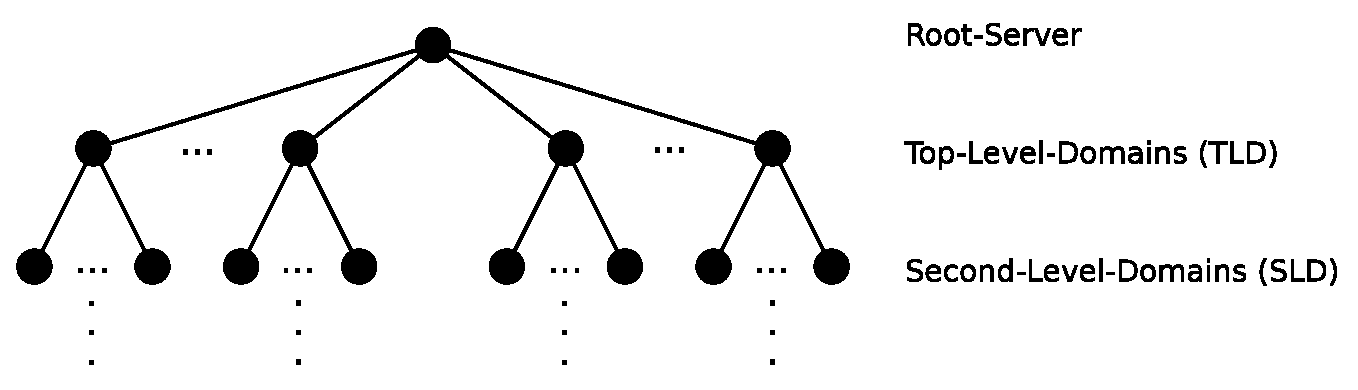
\includegraphics[width=\textwidth]{images/tree}
			\caption{Baumstruktur des \dns{}}
			\label{fig:tree}
		\end{figure}

		%Überleitung

		Ausfallsicherheit, ständige Verfügbarkeit und kurze Antwortzeiten sind Anforderungen, welche
		ebenfalls an viele andere Netzwerk-Dienste gestellt werden. Um diese Anforderungen zu erfüllen,
		gibt es das Konzept der Lastverteilung. Dabei wird eine hohe Last auf einer Ressource dadurch
		verringert, dass die Gesamtlast auf mehrere identische Ressourcen verteilt wird. Auf diese Weise
		ist die Last je Ressource geringer und besser handhabbar. Dieses Konzept wird allgemein in
		Netzwerken und bei Server-Systemen angewendet \cite{bourke2001, kopparapu2002}. Aber auch
		speziellere Anwendungsgebiete, wie die Verteilung von Last auf Webservern, sind besonders
		interessant für Websites mit hohen Lastanforderungen \cite{meplho2012}. Hierbei wird die
		anfallende Last auf ein Cluster aus Backend-Servern verteilt. Jeder der sogenannten
		Backend-Server stellt die gleiche Anwendung bereit. Die Aufgabe der Verteilung übernimmt dabei
		meist ein Lastverteiler, welcher vor den Backend-Servern in das Netzwerk eingefügt wird. Jede
		Anfrage wird somit durch den Lastverteiler geleitet, und dann von diesem an einen verfügbaren
		Backend-Server weitergegeben. Diese allgemeinen Konzepte lassen sich ebenfalls für hohe
		Lastsituationen im DNS nutzen.

		Diese Arbeit beschäftigt sich mit dem Thema der Lastverteilung von DNS-Anfragen. Dazu wird ein
		bestehendes System \cite{zinke2007,scsczile2008,zinke2012,salbnet} zur selbst-adaptiven
		Lastverteilung von TCP-Anfragen so erweitert, dass es ebenfalls UDP-Anfragen verarbeiten kann.
		Dieses System ist in dem Sinne selbst-adaptiv, weil der Lastverteiler keine eigenständigen
		Annahmen über die Last der Backend-Server trifft. Jeder Backend-Server ermittelt eigenständig
		eine Einschätzung der aktuellen Lastsituation, welche dem Lastverteiler über Credits
		mitgeteilt wird. Dabei entspricht ein Credit einer weiteren Verbindung, die von dem Server
		abgearbeitet werden kann. Somit passt sich der Lastverteiler immer eigenständig der aktuellen
		Lastsituation auf den Backend-Servern an, ohne dass ein Administrator Einstellungen am
		Lastverteiler vornehmen muss.  Dadurch unterscheidet sich das System von anderen
		Lastverteilungs-Algorithmen, welche meist initial konfiguriert werden und danach kaum
		beeinflussbar sind. So kann auch eine fehlerhafte initiale Konfiguration nicht im laufenden
		Betrieb ausgebessert werden.

		Das in \cite{zinke2007,scsczile2008} beschriebene System ist für TCP\footnote{Das Transmission
		Control Protocol (TCP) \cite{rfc793} ist ein zuverlässiges, verbindungsorientiertes und
		paketvermitteltes Transportprotokoll der TCP/IP-Suite \cite{stevens1994}. Es wird für
		Verbindungen eingesetzt, welche in dem Sinne verlässlich sind, dass verlorene Datenpakete
		erneut übertragen werden. Um dies zu realisieren, ist allerdings ein gewisser Mehraufwand beim
		Verbindungsaufbau und -abbau nötig.  Bekanntestes Beispiel für TCP-Verbindungen stellen
		HTTP-Anfragen zum Abrufen und Kommunizieren mit Websites dar.}-Anfragen implementiert. Es wurde
		anhand des Apache Webservers (httpd) \cite{httpd} getestet \cite{zinke2012}. Bei diesen Tests
		wurden die Credits über ein InfiniBand-Netzwerk \cite{infiniband,zinke2007} übertragen und direkt
		in den Speicher des Lastverteilers geschrieben\footnote{InfiniBand \cite{infiniband} ist eine
		Hochgeschwindigkeits-Übertragungstechnik, welche zusätzlich Remote Direct Memory Access (RDMA)
		unterstützt. Das ermöglicht einen direkten Speicherzugriff auf einen über das Netzwerk verbunden
		Rechner.}. Durch den direkten Schreibzugriff, muss keine blockierende Kommunikation zwischen dem
		Lastverteiler und dem Backend-Server stattfinden.

		Aufgabe dieser Arbeit ist es, dass bereits für TCP implementierte Verfahren auch für UDP zu
		implementieren. Das User Datagram Protocol (UDP) \cite{stevens1994, rfc768} ist ebenfalls ein
		paketvermitteltes Transportprotokoll aus der TCP/IP-Suite, jedoch im Gegensatz zum TCP,
		verbindungslos und unzuverlässig. Das bedeutet, der Verlust eines Datenpakets während der
		Übertragung wird nicht bemerkt, und somit ist auch keine automatische Wiederholung der Übertragung
		möglich. Diese Eigenschaft grenzt die Anwendungsfälle, in denen UDP sinnvoll einsetzbar ist,
		bereits stark ein, allerdings entfällt durch diese Unzuverlässigkeit der Mehraufwand am Anfang
		und am Ende einer zuverlässigen Verbindung, wie es zum Beispiel bei TCP der Fall ist. Da es sich
		bei DNS-Anfragen immer nur um eine Frage und eine Antwort handelt, welche schnell übertragen
		werden sollen, ist der Mehraufwand einer TCP-Verbindung nicht sinnvoll. Deswegen wird im
		Standardfall für DNS-Anfragen UDP genutzt. Das allgemeine Vorgehen ist dabei so, dass Anfragen,
		welche nicht in einem bestimmten Zeitraum beantwortet wurden, erneut gesendet werden. Diese
		Unterschiede zwischen TCP und UDP müssen bei der Erweiterung des bestehenden Systems beachtet
		werden.  Außerdem wird zur Übertragung der Credits, zwischen den Backend-Servern und dem
		Lastverteiler, eine TCP/IP-Verbindung über Ethernet genutzt. Dadurch soll verdeutlicht werden,
		dass dieses selbst-adaptive System auch über blockierende Kommunikation effizient ist.

		Die Arbeit ist in 8 Kapitel aufgeteilt. Zu Beginn werden in Kapitel \ref{cha:grundlagen} die
		Grundlagen dieser Arbeit erklärt. Es handelt sich dabei um das \dns{} und
		Lastverteilungsansätze.  Darüber hinaus wird eine Einordnung dieser Arbeit in die vorgestellten
		Konzepte vorgenommen.  Anschließend werden in Kapitel \ref{cha:arbeiten} einige Arbeiten
		aufgeführt, welche sich mit DNS-Clustern und Lastsituationen in eben diesen befassen. Das zu
		erweiternde System zur selbst-adaptiven Lastverteilung \textit{salbnet} \cite{zinke2012,salbnet} wird in
		Kapitel \ref{cha:salbnet} beschrieben.  Im \ref{cha:konzept}. Kapitel werden das Konzept der
		erarbeiteten Erweiterung und die dazugehörigen Vorüberlegungen aufgezeigt.  Im darauf folgenden
		Kapitel \ref{cha:implementierung} wird die konkrete Umsetzung des vorher dargestellten Konzepts
		beschrieben.  Es wird hierbei auf Besonderheiten und Probleme bei der Implementation
		eingegangen.  Daran anschließend werden in Kapitel \ref{cha:messungen} die Ergebnisse einer
		Funktionsmessung und eine Einschätzung der Implementation vorgestellt. Am Ende dieser Arbeit
		folgen in Kapitel \ref{cha:zusammenfassung} eine Zusammenfassung, Einschätzung und Bewertung der
		erreichten Ziele und ein Ausblick auf mögliche Erweiterungen des Konzepts.

	% chapter Einleitung }}}

	\chapter{Grundlagen} % {{{
	\label{cha:grundlagen}

		Dieses Kapitel soll eine Einführung in die Verfahren und Techniken geben, die dieser Arbeit
		zu Grunde liegen.  Dazu wird zu Beginn des Kapitels in Abschnitt \ref{sec:dns} auf die Entstehung,
		Bedeutung und Funktionsweise des \dns{} eingegangen. Außerdem werden Softwaresysteme
		vorgestellt, welche zum Betreiben eines DNS-Servers geeignet sind. Daran anschließend soll im
		Abschnitt \ref{sec:lastverteilung} ein Überblick über bestehende Konzepte und Praktiken der
		allgemeinen Lastverteilung gegeben werden, wobei auf Besonderheiten der Lastverteilung für das
		DNS eingegangen wird. Zum Abschluss des Kapitels wird diese Arbeit in Abschnitt
		\ref{sec:grundlagen-fazit} in die vorgestellten Konzepte eingeordnet.

		\section{\dns{}} % {{{
		\label{sec:dns}

		In diesem Abschnitt wird das \dns{} \cite{rfc1034,rfc1035} beschrieben. Dazu wird im ersten
		Abschnitt \ref{sub:entstehung} auf die Entstehung des DNS eingegangen und die Notwendigkeit
		eines solchen Systems dargestellt.  Anschließend folgt in Abschnitt \ref{sub:aufbau} eine
		Erläuterung des heutigen Aufbaus des DNS und seine Nutzung zur Informationsverteilung.
		Zum Schluss wird in Abschnitt \ref{sub:software} auf die bekanntesten und verbreitetsten
		Softwaresysteme eingegangen, welche aktuell zur Bereitstellung eines DNS-Servers genutzt werden.

			\subsection{Entstehung und Bedeutung} % {{{
			\label{sub:entstehung}

			Um die Entstehung des \dns{} zu verstehen, ist es entscheidend zu wissen, wie das Internet
			entstanden und aufgebaut ist.

			Das sogenannte ARPANET ist ein Wide Area Network (WAN) gewesen, welches in den späten
			sechziger Jahren von der Advanced Research Projects Agency (ARPA) des
			Verteidigungsministeriums der USA aufgebaut und finanziert wurde. Es hat mehrere große
			Forschungseinrichtungen in den USA verbunden und diente der Zusammenarbeit und dem Austausch
			von Daten zwischen diesen Einrichtungen. Bereits kurze Zeit nachdem die ersten Computer an
			das ARPANET angeschlossen wurden, begann die Entwicklung der TCP/IP-Suite \cite{stevens1994},
			einer Menge an Protokollen, welche den Transport von Datenpaketen über ein Netzwerk regeln
			und ermöglichen.  Die beiden bekanntesten Protokolle aus dieser Protokollfamilie sind das
			Internet Protocol (IP) \cite{rfc791} und das Transmission Control Protocol (TCP)
			\cite{rfc793}. Anfang der achtziger Jahre wurde die TCP/IP-Suite Standard auf dem ARPANET.
			Gleichzeitig führte die Entwicklung des Berkeley Software Distribution (BSD) Unix
			Betriebssystems, welches die TCP/IP-Suite zur Verfügung stellte, dazu, dass immer mehr
			Rechenzentren und Computersysteme an das ARPANET angeschlossen wurden. Das Resultat dieser Entwicklung
			war, dass aus einer geringen Anzahl von verbundenen Systemen ein großes Netzwerk
			entstand. Dieses Netzwerk entwickelte sich schließlich, mit weiteren anderen Netzwerken, zu
			dem heutigen Internet, einem Netzwerk von Netzwerken.

			Der Sinn eines Netzwerkes ist es, dass die einzelnen Teilnehmer sich kontaktieren und
			Informationen austauschen können. Um das zu ermöglichen, müssen die Netzwerkteilnehmer
			eindeutig identifizierbar sein. Dies ist mit einem Telefonnetz vergleichbar, wo jedem
			Teilnehmer eine eindeutige Kennung, die Telefonnummer, zugewiesen ist. Durch diese Rufnummer
			kann ein Kommunikationspartner mit einem anderen in Verbindung treten. Dasselbe Prinzip gilt
			auch für ein TCP/IP-Netzwerk, wobei jedes verbundene Netzwerkinterface eine eindeutige
			IP-Adresse erhält. Dies ist laut dem IPv4-Standard \cite{rfc791} eine 32-Bit-Adresse, welche
			in der Form \texttt{141.89.249.102} dargestellt wird. Im neueren IPv6-Standard \cite{rfc2460}
			handelt es sich um 128-Bit-Adressen, welche mit der Form \texttt{2a00:1450:4016:800::1010}, im
			Vergleich zu IPv4-Adressen, deutlich komplexer sind und es somit kaum noch für einen Menschen
			möglich ist, sich diese Kennung zu merken. Darüber hinaus benötigt ein Nutzer des Netzwerks
			alle IP-Adressen der Rechner, die er über das Netzwerk erreichen will. Um den Nutzern diese
			Aufgabe abzunehmen, wurde das Prinzip der \texttt{hosts}-Dateien entwickelt, welches einem
			privaten Adressbuch ähnelt. Hierbei existiert eine Datei im lokalen Dateisystem (bei unixoiden
			Systemen die Datei \texttt{/etc/hosts}), welche bekannten IP-Adressen einen beliebigen Namen
			zuweist. Ein Beispiel für eine \texttt{/etc/hosts}-Datei ist in Listing \ref{lst:hosts} zu
			sehen. In ihr sind 2 Namen für den lokalen Rechner (Zeile 6-7) und 2 Namen für andere Geräte
			im Netzwerk (Zeile 8-9) definiert. Dadurch ist es dem Nutzer möglich andere
			Netzwerk-Teilnehmer über den zugewiesenen Namen zu kontaktieren. Der Nutzer bräuchte im
			Beispiel nur noch den Namen \textit{router} verwenden, wenn er auf das Gerät mit der
			IP-Adresse \texttt{192.168.1.1} zugreifen möchte. Das Betriebssystem nutzt dann die
			\texttt{hosts}-Datei um die entsprechende IP-Adresse zu ermitteln. Ein weiterer Vorteil dieses
			Vorgehens besteht darin, dass, wenn sich die IP-Adresse eines der Geräte im Netzwerk ändert,
			ein Anpassen der \texttt{/etc/hosts}-Datei ausreicht. Der Nutzer muss sich nicht die neue
			Adresse merken und kann weiterhin, wie gewohnt, den in der \texttt{hosts}-Datei definierten
			Namen einsetzen. Für ein kleines statisches Netzwerk ist dies eine durchaus ausreichende
			Lösung. Jedoch wuchs das ARPANET relativ schnell, was dazu führte das lokale
			\texttt{hosts}-Dateien keine sinnvolle Lösung mehr waren. Der nächste Schritt war es ein
			zentrales Verzeichnis bereitzustellen. Dies wurde durch die \texttt{HOSTS.TXT} realisiert,
			welche vom Network Information Center (NIC) des Stanford Research Institute (SRI) gepflegt
			wurde. Dieses Verzeichnis wurde zentral zur Verfügung gestellt, sodass jeder Netzwerk-Nutzer
			immer die aktuelle Version erhalten und daraus seine lokale \texttt{hosts}-Datei generieren
			konnte.  Dieser zentrale Ansatz hatte den Vorteil, dass schnell auf Änderungen reagiert werden
			konnte, diese leicht zu verteilen waren und Nameskonflikte verhindert wurden.  Allerdings ist
			auch dieser Ansatz nicht für ein Netzwerk in der Größe des heutigen Internet handhabbar.  Der
			Zeitaufwand zum Instandhalten und der Netzwerkverkehr zum Verteilen wären heutzutage nicht
			mehr vertretbar. Um diese Probleme zu lösen, wurde das DNS \cite{rfc1034} entwickelt, welches
			durch einen dezentralen Ansatz die Informationen und deren Pflege verteilt.

			\lstinputlisting[float,language=sh,caption={Beispiel \texttt{/etc/hosts}-Datei mit 4 Einträgen},label=lst:hosts]{listings/hosts}

			% subsection Entstehung und Bedeutung }}}

			\subsection{Aufbau} % {{{
			\label{sub:aufbau}

			Das \dns{} ersetzte 1987 das zentrale Verzeichnis \texttt{HOSTS.TXT}. Wie bereits in Kapitel
			\ref{cha:einleitung} beschrieben, basiert es auf einem dezentralen Ansatz, bei dem die
			Informationen in einer baumartigen Struktur gespeichert werden. So ein Baum ist auszugsweise
			in Abbildung \ref{fig:dns-tree} zu sehen. Diese Struktur des Baums, also die Knoten, sind auch
			in den Domain-Namen zu erkennen. Ein Domain-Name besteht aus mehreren Subdomains, welche durch
			Punkte getrennt sind und jeweils einem Knoten im Baum entsprechen. So besteht zum Beispiel die
			Domain \texttt{cs.uni-potsdam.de} aus den Subdomains \texttt{cs}, \texttt{uni-potsdam},
			\texttt{de} und der Root-Domain, welche meist entfällt bzw. als leere Zeichenkette
			(\glqq{}\grqq{}) dargestellt wird.

			Der Vorteil der Speicherung der DNS-Informationen in einem Baum besteht darin, dass jede Subdomain
			nur Informationen zu dem darunter liegenden Teilbaum speichern muss. Das heißt, die Subdomain
			\texttt{de} besitzt Informationen bezüglich den Subdomains \texttt{denic} und
			\texttt{uni-potsdam}, aber keine Informationen bezüglich \texttt{com} oder \texttt{net}.
			Dadurch wird einerseits die Menge an Informationen je Knoten gering gehalten, und außerdem
			kann so die Verwaltung und Pflege der Information an verschiedene Betreiber delegiert werden.

			Die Root-Domain, welche aktuell von 13 Root-Servern \cite{rootserver} bereitgestellt wird,
			steht unter der Kontrolle der Internet Corporation for Assigned Names and Numbers (ICANN). Auch
			die Vergabe der Top-Level-Domains (TLDs) ist an sie gebunden. Die ICANN ist eine
			Non-Profit-Organisation mit Sitz in den USA. Sie ist zwar für die Vergabe der TLDs
			verantwortlich, verwaltet und betrieben werden diese jedoch von verschieden Organisationen und
			Unternehmen. Es existieren aktuell 313 TLDs \cite{tlds}, welche sich hauptsächlich in folgende
			Arten unterteilen lassen:

			\begin{itemize}
				\item länderspezifische \textit{country-code TLDs} (ccTLDs) und
				\item allgemeine \textit{generic TLDs} (gTLDs):
				\begin{itemize}
					\item von ICANN verwaltete \textit{unsponsored TLDs} (uTLDs),
					\item von privaten Organisationen vorgeschlagene \textit{sponsored TLDs} (sTLDs).
				\end{itemize}
			\end{itemize}

			\begin{figure}
				\centering
				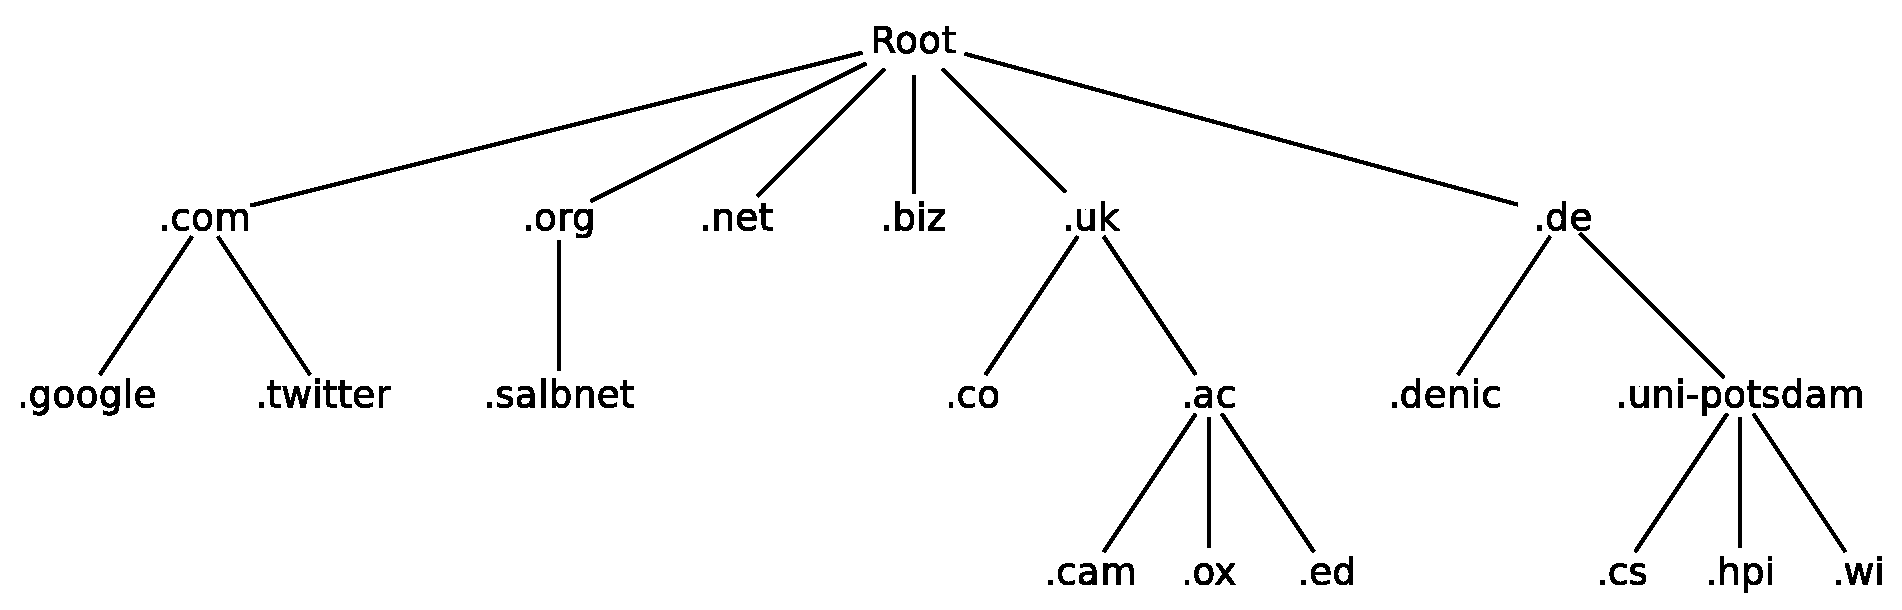
\includegraphics[width=\textwidth]{images/dns-tree-domains}
				\caption{Ausschnitt aus der DNS-Topologie}
				\label{fig:dns-tree}
			\end{figure}


			In der Abbildung \ref{fig:dns-tree} sind zum Beispiel die Domains \texttt{uk}, \texttt{fr} und \texttt{de}
			ccTLDs, die Domains \texttt{com}, \texttt{org} und \texttt{net} sind uTLDs, und \texttt{mobi}
			ist eine sTLD. Unter den TLDs folgen die sogenannten Second-Level-Domains (SLDs), welche meist
			schon zu den eigentlichen Netzteilnehmern gehören oder noch eine weitere Einteilungsebene
			einführen. So gibt es zum Beispiel in der englischen \texttt{uk}-Domain noch die
			\texttt{co}-Domain für Firmen oder die \texttt{ac}-Domain für akademische Einrichtungen. Die
			\texttt{uni-potsdam}-Domain in der \texttt{de}-Domain wird allerdings bereits direkt von der
			Universität Potsdam verwaltet. Die Universität Potsdam unterteilt ihre eigene SLD wiederum
			weiter in Subdomains, zum Beispiel für die einzelnen Institute (\texttt{cs} für das Institut
			für Informatik). Diese Domains können dann wiederum von den einzelnen Instituten verwaltet und
			weiter unterteilt werden.

			\lstinputlisting[float,caption={Ausschnitt eines Master-Files},label=lst:master]{listings/master-file}

			Dieser dezentrale Ansatz hat eine Reihe von Vorteilen. Als wichtigster Punkt ist die
			Verteilung der Last zu nennen, womit sowohl der Aufwand zur Wartung einer Domain, als auch zur
			Verteilung der Informationen gemeint ist. Außerdem ist es für die Betreiber einer Domain
			einfacher Änderungen einzupflegen. Da ein Betreiber alle Subdomains seiner eigenen Domain
			allein verwalten kann, spricht man dabei von einer \textit{Zone}.
			Eine Zone umfasst alle Domains, die von diesem DNS-Betreiber administriert werden. So gehören
			alle Subdomains von \texttt{haiti.cs.uni-potsdam.de} zum Beispiel zu einer Zone. Diese Zonen
			werden über sogenannte Master-Files \cite{rfc1035,liualb2006} konfiguriert. Listing
			\ref{lst:master} zeigt einen Auszug aus einem Beispiel für ein Master-File. Der grundlegende
			Aufbau ist in der Form: Domain-Name (vollständig mit abschließendem Punkt oder Subdomain),
			Klasse (IN für Internet), Typ (optionale weitere Parameter für spezielle Typen z.B. bei MX)
			und abschließend die gespeicherte Information. In Listing \ref{lst:master} sind in Zeile 1-2
			zwei \texttt{NS}-Einträge. Diese geben die Nameserver einer Domain an. In Zeile 4 ist ein Eintrag
			für einen Mailserver (\texttt{MX}). Er enthält zusätzlich einen Präferenz-Wert (10),
			welcher bei mehreren Mailservern die Ordnung dieser definiert. Anschließend folgen in Zeile
			6-9 vier IPv4-Adressen (\texttt{A}) für verschiedene Subdomains. Und in Zeile 11 ist der Alias
			(\texttt{CNAME}) \textit{www} für die  \textit{twix}-Domain definiert. Dieses Beispiel zeigt
			nur eine kleine Anzahl von möglichen Typen, weshalb in Tabelle \ref{tab:dns-types} die
			wichtigsten von ihnen aufgeführt sind.


			\begin{table}
				\centering
				\begin{tabular}{|c|l|}\hline
					Typ & Beschreibung \\\hline\hline
					A & IPv4-Adresse\\
					AAAA & IPv6-Adresse\\
					NS & Nameserver\\
					MX & Mailserver\\
					CNAME & Kanonischer Name eines Alias\\
					SOA & Start einen Zonenautorität\\
					PTR 	& Zeiger von eine Adresse auf eine Domain\\\hline
				\end{tabular}
			\caption{Die wichtigsten Eintragstypen in einem DNS-Master-File \cite{rfc1035,rfc3596}}
			\label{tab:dns-types}
			\end{table}

			Diese Master-Files werden von DNS-Servern gelesen und verarbeitet. Es gibt verschiedene Arten
			von DNS-Servern, die bestimmen, wie der DNS-Server auf Anfragen antwortet. Dabei
			unterscheidet man iterative und rekursive Nameserver.

			\subsubsection*{Iterative Nameserver} % {{{

			Ein iterativer Nameserver kennt nur die Informationen aus seinem eigenen Master-File, also
			seiner eigenen Zone. Erhält ein iterativer Nameserver eine Anfrage außerhalb seiner Zone, kann
			er diese nicht beantworten und sendet deshalb die Adressen der Server zurück, welche für die
			Root-Domain verantwortlich sind. Diese Adressen sind jedem DNS-Server bekannt. Das Ziel dieses
			Verhaltens ist es, auf dem DNS-Server keine unnötige Last zu erzeugen und die Antwortzeit so
			gering wie möglich zu halten. Daraus lässt sich auch der Haupteinsatzort für solche Nameserver
			ableiten. Alle Server, welche die Root-Domain und die TLDs verwalten, sind iterative
			Nameserver. Sie erhalten die meisten Anfragen und müssen diese schnell und effizient
			verarbeiten. Auch die meisten DNS-Server von Firmen, welche durch das Internet erreichbar
			sind, werden ebenfalls iterative Nameserver sein.

			% subsubsection Iterative Nameserver }}}

			\subsubsection*{Rekursive Nameserver} % {{{

			Das Gegenteil zu iterativen sind rekursive Nameserver. Auch sie beantworten Anfragen bezüglich
			der eigenen Zone. Wenn sie jedoch eine Anfrage außerhalb ihrer Zone erhalten, erfragen sie die
			Antwort selbst bei anderen Nameservern. Das heißt, der gefragte rekursive Nameserver
			unternimmt den Aufwand und ermittelt selbst die Antwort auf die gestellte Frage. Er sendet
			diese dann an den Fragenden zurück. Um dieses Vorgehen effizienter zu gestalten, werden häufig
			Caches eingesetzt. In ihnen werden die ermittelten Informationen, welche außerhalb der eigenen
			Zone liegen, gespeichert. Dadurch können Anfragen schneller beantwortet werden, falls die
			Antwort bereits im Cache existiert. Falls dies nicht der Falls ist, kann trotzdem schneller
			die Antwort gefunden werden, falls im Cache bereits Informationen zu einem Nameserver in der
			Nähe der Domain existieren. Das heißt, wenn die Domain \texttt{haiti.cs.uni-potsdam.de}
			angefragt wird und im Cache bereits die Adresse des \texttt{uni-potsdam.de}-Nameservers
			gespeichert ist, kann die Antwort schneller gefunden werden, als wenn der Nameserver sich von
			der Root-Domain durchfragen müsste.

			Rekursive Nameserver werden vor allem in privaten Netzwerken eingesetzt, wie zum Beispiel
			Heimnetzwerke oder firmeninternen Netzwerke, aber auch bei Internet Service Providern
			(ISPs). An diesen Punkten im Internet ist der Einsatz rekursiver Nameserver am sinnvollsten,
			denn dort treffen häufig die gleichen oder zu mindestens ähnliche Anfragen ein. So kann man
			oft davon ausgehen, dass diese Nameserver immer die aktuelle Adresse von \texttt{google.com} und
			\texttt{wikipedia.org} etc. im Cache gespeichert haben. Dieses Speichern von Informationen
			ist nicht nur vorteilhaft für die Nutzer, sondern verringert auch die Last auf anderen
			DNS-Servern im Internet. Ohne Nameserver mit Cache ist die Last auf dem DNS-Netzwerk wohl um
			einiges höher. Allerdings sind die Informationen eines DNS-Servers nur begrenzt gültig.
			Jede Antwort enthält eine maximale Lebensdauer der Information, danach ist sie nicht mehr
			gültig und sollte nicht weiterverwendet werden. Das heißt auch, dass sie aus dem Cache entfernt
			und neu abgefragt werden muss. Dies ist jedoch nötig, da sonst nie Änderungen innerhalb einer Zone
			weiter propagiert würden.

			% subsubsection Rekursive Nameserver }}}

			\subsubsection*{Resolver} % {{{

				\begin{figure}
					\centering
					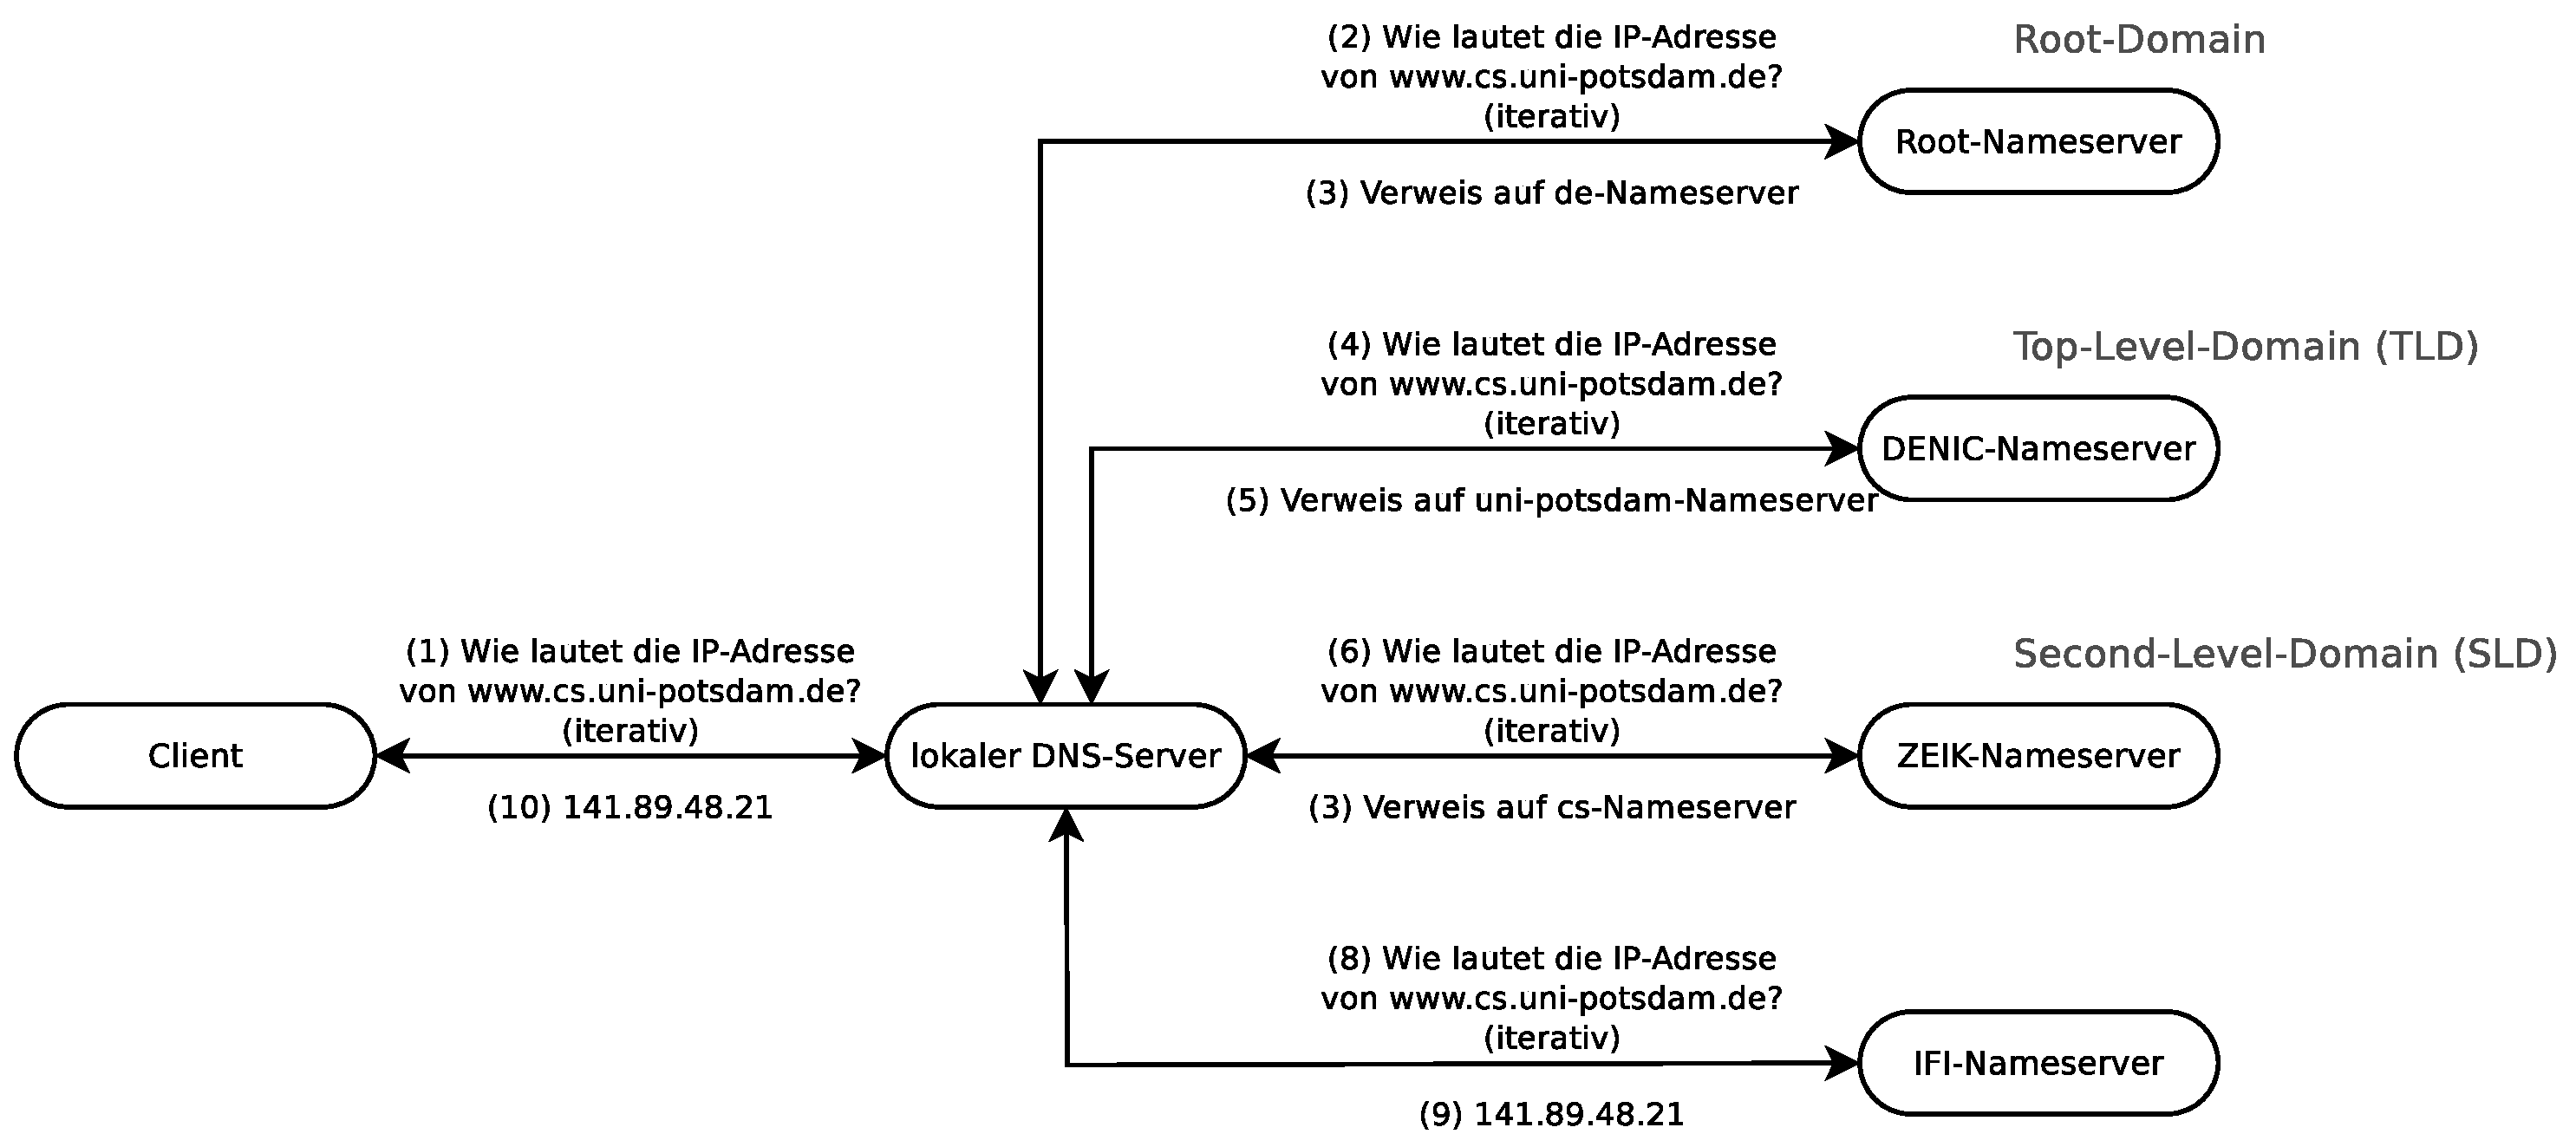
\includegraphics[width=\textwidth]{images/request}
					\caption{DNS-Anfragen für \texttt{www.cs.uni-potsdam.de}}
					\label{fig:bsp-request}
				\end{figure}

				Damit eine Anwendung, wie zum Beispiel ein Webbrowser oder ein E-Mail-Client, Adressen
				auflösen kann, wird ein sogenannter Resolver benötigt. Seine Aufgabe ist es, für die
				Anwendung einen Domain-Namen zu der entsprechenden IP-Adresse aufzulösen. Das heißt, wenn
				der Resolver von einer Anwendung die Anfrage nach der Adresse \texttt{www.cs.uni-potsdam.de}
				erhält, erzeugt der Resolver eine gültige DNS-Anfrage \cite{rfc1035} nach eben dieser
				Adresse und sendet sie an den im Betriebssystem konfigurierten primären DNS-Server. Dabei
				handelt es sich meist um einen rekursiven Nameserver, welcher dann selber einen Resolver
				nutzt, um weitere Anfragen zu stellen, sofern er die Antwort nicht im Cache gespeichert hat.
				In Abbildung \ref{fig:bsp-request} ist der Ablauf der Beispiel-Anfrage dargestellt. Der
				Resolver des Clients sendet die Anfrage (1) an den lokalen DNS-Server. Dieser ist rekursiv
				und ermittelt deshalb nun die Antwort\footnote{Annahme: Der Cache des DNS-Servers enthält
				keine relevanten Informationen.}. Die Anfrage (2) wird deshalb an einen Root-Nameserver
				gestellt, da der lokale DNS keine anderen Informationen bezüglich der Domain besitzt. Der
				Root-Nameserver besitzt nur die Information, welcher Nameserver für die \texttt{de}-Domain
				verantwortlich ist und sendet diese Antwort (3) an den lokalen DNS-Server zurück. Dieser
				befragt (4) anschließend den \texttt{de}-Nameserver, welcher wiederum ein iterativer
				Nameserver ist und somit nur die \texttt{uni-potsdam}-Domain kennt (5). Die Anfragen an den
				\texttt{uni-potsdam}-Nameserver (6) liefert die Adresse des zuständigen Nameservers zurück
				(7). Dieser kann nun auf die letzte Anfrage (8) mit der gewünschten Adresse antworten (9)
				und der lokale DNS-Server liefert sie an den Client zurück (10). Alle Informationen, die in
				den Zwischenanfragen gesammelt wurden, werden im Cache des lokalen DNS-Servers gespeichert.
				Würde nun der Client erneut nach der Adresse \texttt{www.cs.uni-potsdam.de} fragen, könnte
				der lokale DNS-Server sofort antworten. Oder wenn die Anfrage diesmal
				\texttt{haiti.cs.uni-potsdam.de} wäre, würde der lokale DNS-Server sofort beim
				\texttt{cs.uni-potsdam.de}-Nameserver anfragen, da er dessen Adresse bereits kennt und weiß,
				dass dieser für die Domain zuständig ist.

			% subsubsection Resolver }}}

			\subsubsection*{DNS Security Extension} % {{{

				Mit der DNS Security Extension (DNSSEC) \cite{rfc4033,rfc4034,rfc4035,liualb2006} wurde ein
				neuer Standard eingeführt, welcher das DNS absichern soll. Es gibt verschiedene
				Angriffsszenarien auf das DNS \cite{lorenz2012}, wodurch Informationen verändert und somit
				ganze Domains übernommen werden können. Mit DNSSEC soll die Authentizität und
				Datenintegrität der Informationen gewährleistet werden und überprüfbar sein. Dazu werden
				kryptographische Verfahren eingesetzt. Die Einführung und Umstellung auf DNSSEC ist zu
				diesem Zeitpunkt noch nicht abgeschlossen, jedoch ergeben sich daraus interessante
				Überlegungen bezüglich der Last auf dem DNS-Netzwerk. Durch die kryptographische
				Absicherung werden die DNS-Nachrichten größer und Resolver müssen kryptographische
				Methoden nutzen, was eine höhere Rechenleistung beim Client voraussetzt. Sobald das
				System vollständig eingeführt wurde, wird es interessant sein zu untersuchen, in welcher
				Form sich die Veränderung auf die Auslastung des DNS auswirkt.

			% subsubsection DNSsec }}}

			% subsection Aufbau }}}

			\subsection{DNS-Server Software} % {{{
			\label{sub:software}

				In diesem Abschnitt werden mehrere Softwaresysteme vorgestellt, welche zum Betrieb eines
				DNS-Server genutzt werden können. Diese wurden aufgrund von zwei Studien aus den Jahren 2004
				und 2009 zur Verteilung von DNS-Server-Software ausgewählt. Die erste Studie
				\cite{survey2004} wurde am 23. Mai 2004 abgeschlossen und untersuchte 37.836.997 SLDs unter
				den TLDs \texttt{com}, \texttt{net}, \texttt{org},	\texttt{info} und \texttt{biz}. Die
				zweite Studie \cite{survey2009} ist von Oktober 2009. In ihr wurden 3.308.662 SLDs unter den
				TLDs \texttt{com}, \texttt{net} und \texttt{org} untersucht. Man versuchte jeweils die
				Version der eingesetzten DNS-Server-Software zu ermitteln. Dabei wurden die Systeme BIND,
				djbdns, Microsoft DNS und NSD als vier der häufigsten Systeme ermittelt (siehe Tabelle
				\ref{tab:verteilung}). Die genannten vier Systeme werden im Folgenden vorgestellt.
				Zusätzlich wird auf den dnsmasq Server eingegangen, welcher eine sehr spezielle Form eines
				DNS-Servers darstellt.

				\begin{table}
					\centering
					\begin{tabular}{|c|r|r|}\hline
						DNS-Server & \multicolumn{1}{c|}{2004} & \multicolumn{1}{c|}{2009} \\\hline\hline
						BIND & \unit[70,11]{\%} & \unit[73,85]{\%} \\
						djbdns & \unit[15,57]{\%} & \unit[2,56]{\%} \\
						Microsoft DNS & \unit[6,24]{\%} & \unit[0,26]{\%}\\
						NSD & \unit[0,20]{\%} & \unit[0.03]{\%} \\\hline
					\end{tabular}
					\caption{Verteilung von DNS-Server Software nach \cite{survey2004, survey2009}}
					\label{tab:verteilung}
				\end{table}

				\subsubsection*{BIND} % {{{

				Die erste Version des Berkeley Internet Name Domain (BIND) \cite{bind} Server wurde
				Anfang der achtziger Jahre an der University of California, Berkeley entwickelt und mit
				4.3BSD erstmals veröffentlicht. Inzwischen wird BIND von dem Internet Systems Consortium
				(ISC) weiterentwickelt und gepflegt. BIND hat sich zu dem De-facto-Standard für DNS-Server
				entwickelt. Er wird auf 10 der 13 Root-Server eingesetzt und ist auch sonst bei TLDs
				weitverbreitet. Die erste Version des aktuellen BIND 9 Servers wurde 2000 veröffentlicht.
				Ein Nachfolger wird seit 2 Jahren entwickelt, um die aktuellsten Standards (z.B. DNSSEC) zu
				unterstützen.

				Für diese Arbeit wurde der BIND Server als DNS-Server gewählt, da er der weitverbreitetste
				ist und ebenfalls am Institut für Informatik der Universität Potsdam eingesetzt wird.
				Dadurch konnten Testmessungen in einem realistischen Umfeld mit realen Server-Logs
				ausgeführt werden.

				% subsubsection BIND }}}

				\subsubsection*{Name Server Daemon (NSD)} % {{{

				Der Name Server Daemon (NSD) \cite{nsd} wird von den NLnet Labs entwickelt und sein
				Hauptziel ist die Vielfalt unter den Root-Servern zu erhöhen.  Das soll dazu führen, dass
				nicht alle Root-Server durch einen Fehler im BIND Server angreifbar sind. Aktuell nutzen
				auch bereits 3 der 13 Root-Server den NSD als DNS-Server.  Mit der Zielsetzung, vor allem
				auf Root-Servern und TLD-Servern eingesetzt zu werden, erklären sich auch die meisten
				Charakteristiken des NSD. Er ist ausschließlich ein autoritativer DNS-Server, das heißt, er
				beantwortet keine rekursiven Anfragen. Dadurch ist sein Einsatz als DNS-Server in einem
				lokalen Netzwerk ausgeschlossen. Bei dem NSD kann deshalb auf unnötige Funktionen verzichtet
				und somit auf hohe Belastbarkeit optimiert werden. Die erste Version des aktuellen NSD 3
				wurde 2006 veröffentlicht.

				% subsubsection Name Server Daemon (NSD) }}}

				\subsubsection*{Microsoft DNS} % {{{

				Der Microsoft DNS Server \cite{msdns} ist eine Implementation von Microsoft, welche mit den
				Windows Server Produkten ausgeliefert wird. Er kann als autoritativer und rekursiver
				Nameserver betrieben werden. Durch seinen Einsatz auf Windows Servern kommt er vor allem in
				lokalen und Firmen-Netzwerken vor. Ein besonderes Merkmal des Microsoft DNS Servers ist,
				dass die DNS-Informationen nicht nur aus einem Master-File gelesen werden, sondern auch aus
				einem Active Directory stammen können.

				% subsubsection Microsoft DNS }}}

				\subsubsection*{djbdns} % {{{

				Das von Daniel J. Bernstein entwickelte Softwarepaket djbdns \cite{djbdns} ist eines der am
				häufigsten benutzten Systeme zum Betrieb eines DNS-Servers. Daniel J.  Bernstein ist ein
				Mathematiker, Programmierer und Kryptologe aus den USA. Er veröffentlichte djbdns im Jahr
				2001 und setzte eine Belohung \cite{guarantee} von \$1000 aus, für den ersten, der einen
				Fehler in djbdns findet. Die Besonderheit von djbdns liegt darin, dass es ein Softwarepaket
				aus mehreren Programmen ist, welche immer einen speziellen Einsatzzweck erfüllen. Somit
				verringert sich die Code-Basis und die Komplexität der Programme. Die Hauptkomponenten sind
				\texttt{tinydns}, ein autoritativer, und \texttt{dnscache}, ein rekursiver
				Nameserver. Für andere Funktionen, wie das Austauschen von kompletten Zone-Informationen oder
				Blacklisting, existieren ebenfalls eigene Programme.

				% subsubsection Djbdns }}}

				\subsubsection*{dnsmasq} % {{{

				Das Programm dnsmasq \cite{dnsmasq} wird ausschließlich für Heimnetzwerke entwickelt. Es
				stellt DNS- und DHCP\footnote{Das Dynamic Host Configuration Protocol (DHCP) \cite{rfc2131}
				ermöglicht es, Clients in einem Netzwerk dynamisch IP-Adressen zuzuweisen. So kann zum
				Beispiel in einem Heimnetzwerk auf die Konfiguration von statischen IP-Adressen verzichtet
				werden.}-Dienste für ein kleines Netzwerk zur Verfügung. Die Grundidee besteht darin, dass dnsmasq
				die Netzwerkknoten im Heimnetz über DNS verfügbar macht, indem es entweder die
				\texttt{/etc/hosts} oder DHCP Informationen nutzt. Dadurch müssen die lokalen Rechner keine
				eigene \texttt{hosts}-Datei pflegen.  Zusätzlich bietet es einen einfachen Cache für
				DNS-Anfragen, was zu einer Beschleunigung im lokalen Netz führen kann. Somit ist dnsmasq
				kein üblicher DNS-Server und eignet sich auch nicht zum Verwalten von Domains, zeigt jedoch
				eine alternative resourcenschonende lokale Verwendung des DNS auf.

				% subsubsection Dnsmasq }}}

			% subsection DNS-Server Software }}}

		% section Domain Name System (DNS) }}}

		\section{Lastverteilung} % {{{
		\label{sec:lastverteilung}

		\begin{figure}
			\centering
			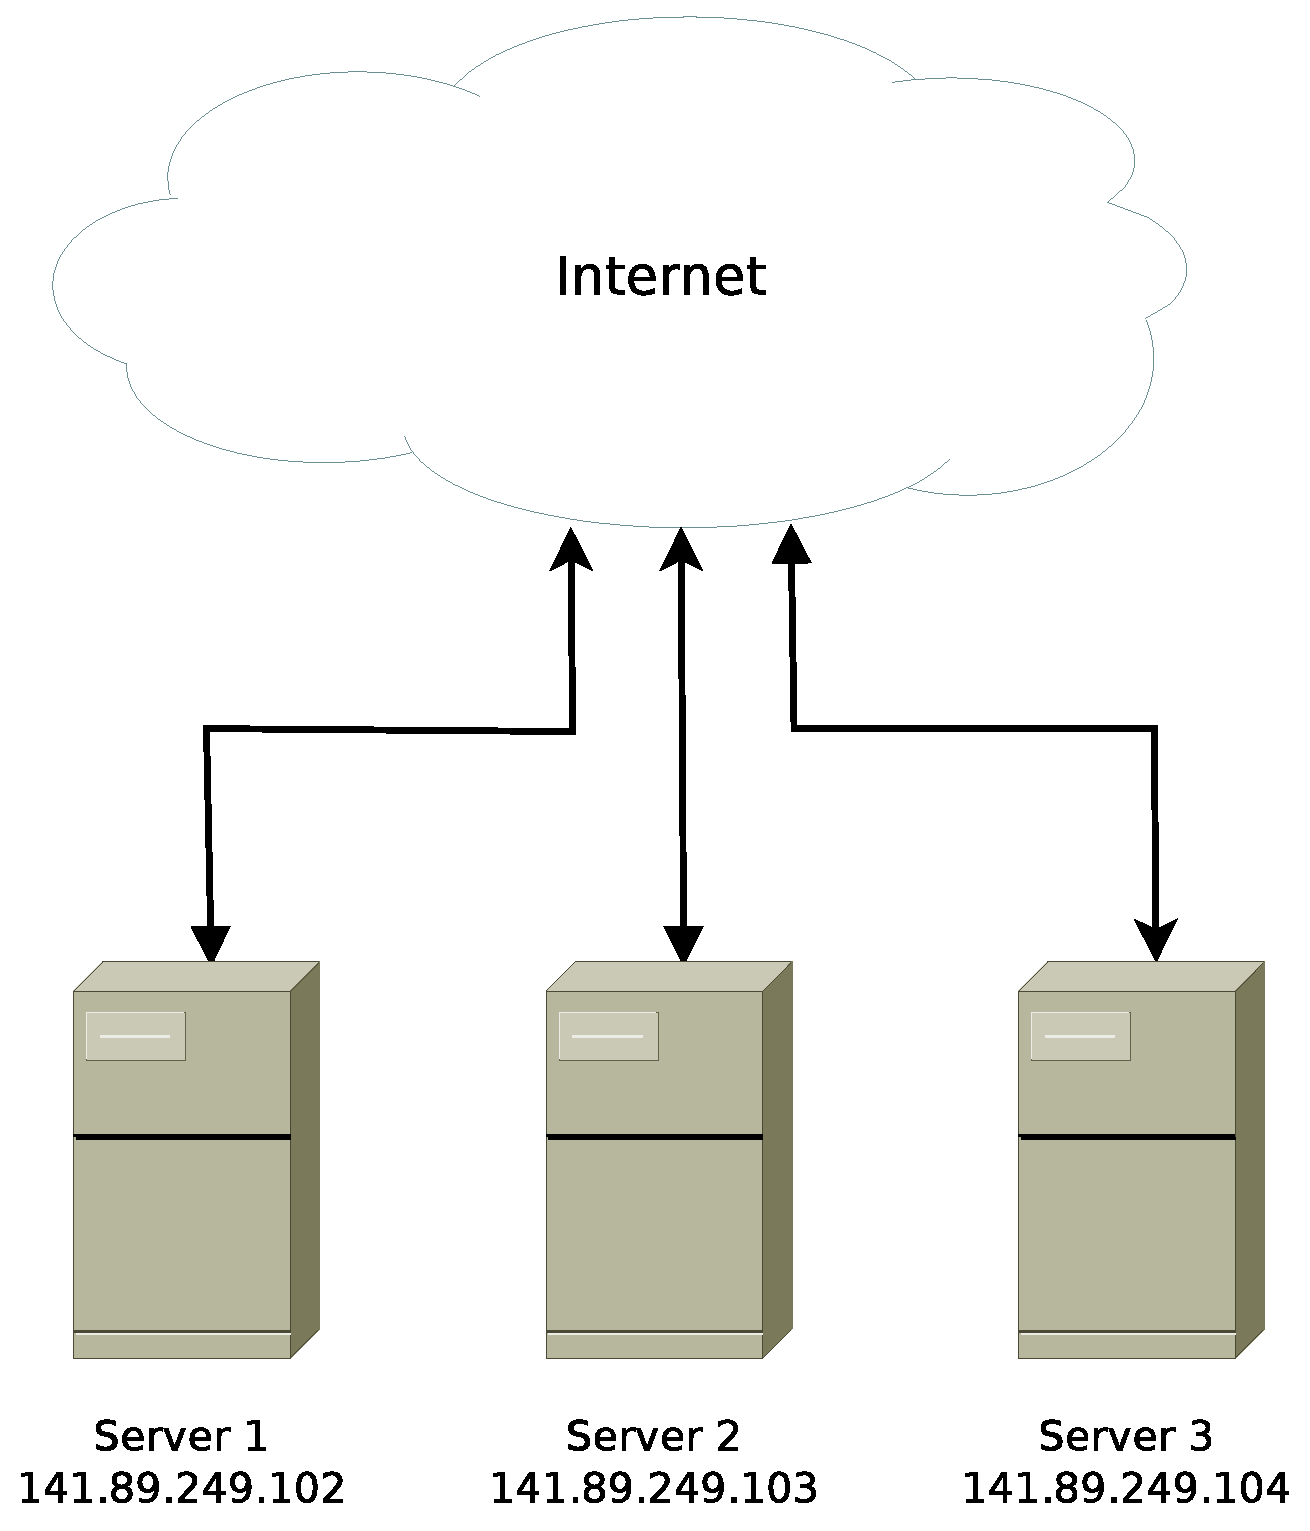
\includegraphics[width=10cm]{images/internet-server}
			\caption{Lastverteilung mit mehreren Servern}
			\label{fig:lastverteilung}
		\end{figure}

		In diesem Abschnitt sollen Problemlösungen vorgestellt werden, welche dazu dienen die Last einer
		einzelnen Netzwerkressource zu verringern. Dies ist immer dann nötig und sinnvoll, wenn eine
		einzelne Ressource im Netzwerk einer so hohen Last ausgesetzt ist, dass sie diese nicht mehr
		allein abarbeiten kann. Bei zu hoher Last können einzelne Anfragen an die Ressource nicht mehr
		beantwortet werden oder im ungünstigsten Fall droht ein Totalausfall. Ein Beispiel für hohe
		Lastsituationen sind Webserver, welche ab einer gewissen Anzahl von Anfragen pro Sekunde nicht
		mehr in der Lage sind, alle abzuarbeiten. Um die Überlastung einzelner Ressourcen zu verhindern
		gibt es zwei Möglichkeiten. Die erste Variante ist, die entsprechende Ressource durch eine
		leistungsfähigere Variante auszutauschen. Dies wird oft bei Datenbanken genutzt, wo der Server
		durch neue Hardware und bessere Ausstattung erweitert wird.  Für Datenbanken ist dies oft die
		einfachere Lösung, da es problematisch sein kann, sie zu verteilen und dabei die Daten
		konsistent zu halten. Die andere Variante ist eine Skalierung in die Breite, das heißt, zum
		Beispiel weitere Server bereitzustellen. So kann der Dienst des Servers, wie in Abbildung
		\ref{fig:lastverteilung} zu sehen ist, von mehreren Servern dem Internet bereitgestellt werden.
		Dieses Vorgehen eignet sich oft bei Webservern, welche durch die Auslieferung von dynamischen
		Inhalten (z.B. PHP-Seiten) ausgelastet sind. Das Skalieren in die Breite bietet Vorteile
		gegenüber der ersten Variante und ist deshalb dieser vorzuziehen, sofern es die Anwendung
		zulässt. Allein durch die Bereitstellung eines zusätzlichen Servers ist es einfacher, einzelne
		Server zu warten und die Gefahr eines Totalausfalls verringert sich. Durch diese Verteilung kann
		ein einzelner Server ausfallen oder überprüft werden, währende der andere Server die Anwendung
		weiterhin zur Verfügung stellt. Zudem ist die Erweiterbarkeit zur weiteren Skalierung einfacher,
		wenn bereits die Infrastruktur geschaffen wurde, mehrere Server zu nutzen. Dieses Variante ist
		im Vergleich zur vorherigen kostengünstiger, da die Anschaffung zweier identischer Systeme meist
		preiswerter als ein einzelnes System ist, welches die gleiche Last verarbeiten kann.  Hinzu
		kommt die Möglichkeit, gezielt Ressourcen zu entfernen, um Strom zu sparen. So könnten Server
		nur dann angeschaltet werden, wenn davon auszugehen ist, dass eine hohe Last bevorsteht. Ein
		Beispiel hierfür ist eine Verkaufsplattform, die zusätzliche Ressourcen benötigt, wenn zum
		Beispiel vor Feiertagen eine hohe Anzahl Bestellungen eingeht.

		Im Folgenden werden verschiedene Ansätze zur Verteilung von Last auf mehrere Systeme erläutert.
		Sie unterscheiden sich in der Umsetzung der Lastverteilung und bieten jeweils gewisse Vor- und
		Nachteile. Die Hauptanwendung für diese Systeme ist die Verteilung von HTTP-Anfragen.
		Diese unterscheiden sich von DNS-Anfragen in mehreren Punkten, weshalb anschließend noch
		Besonderheiten und existierende Verfahren der Lastverteilung von DNS-Verkehr erklärt werden.

			\subsection{Server-Lastverteilung} % {{{
			\label{sub:Server-Lastverteilung}

			\begin{figure}
				\centering
				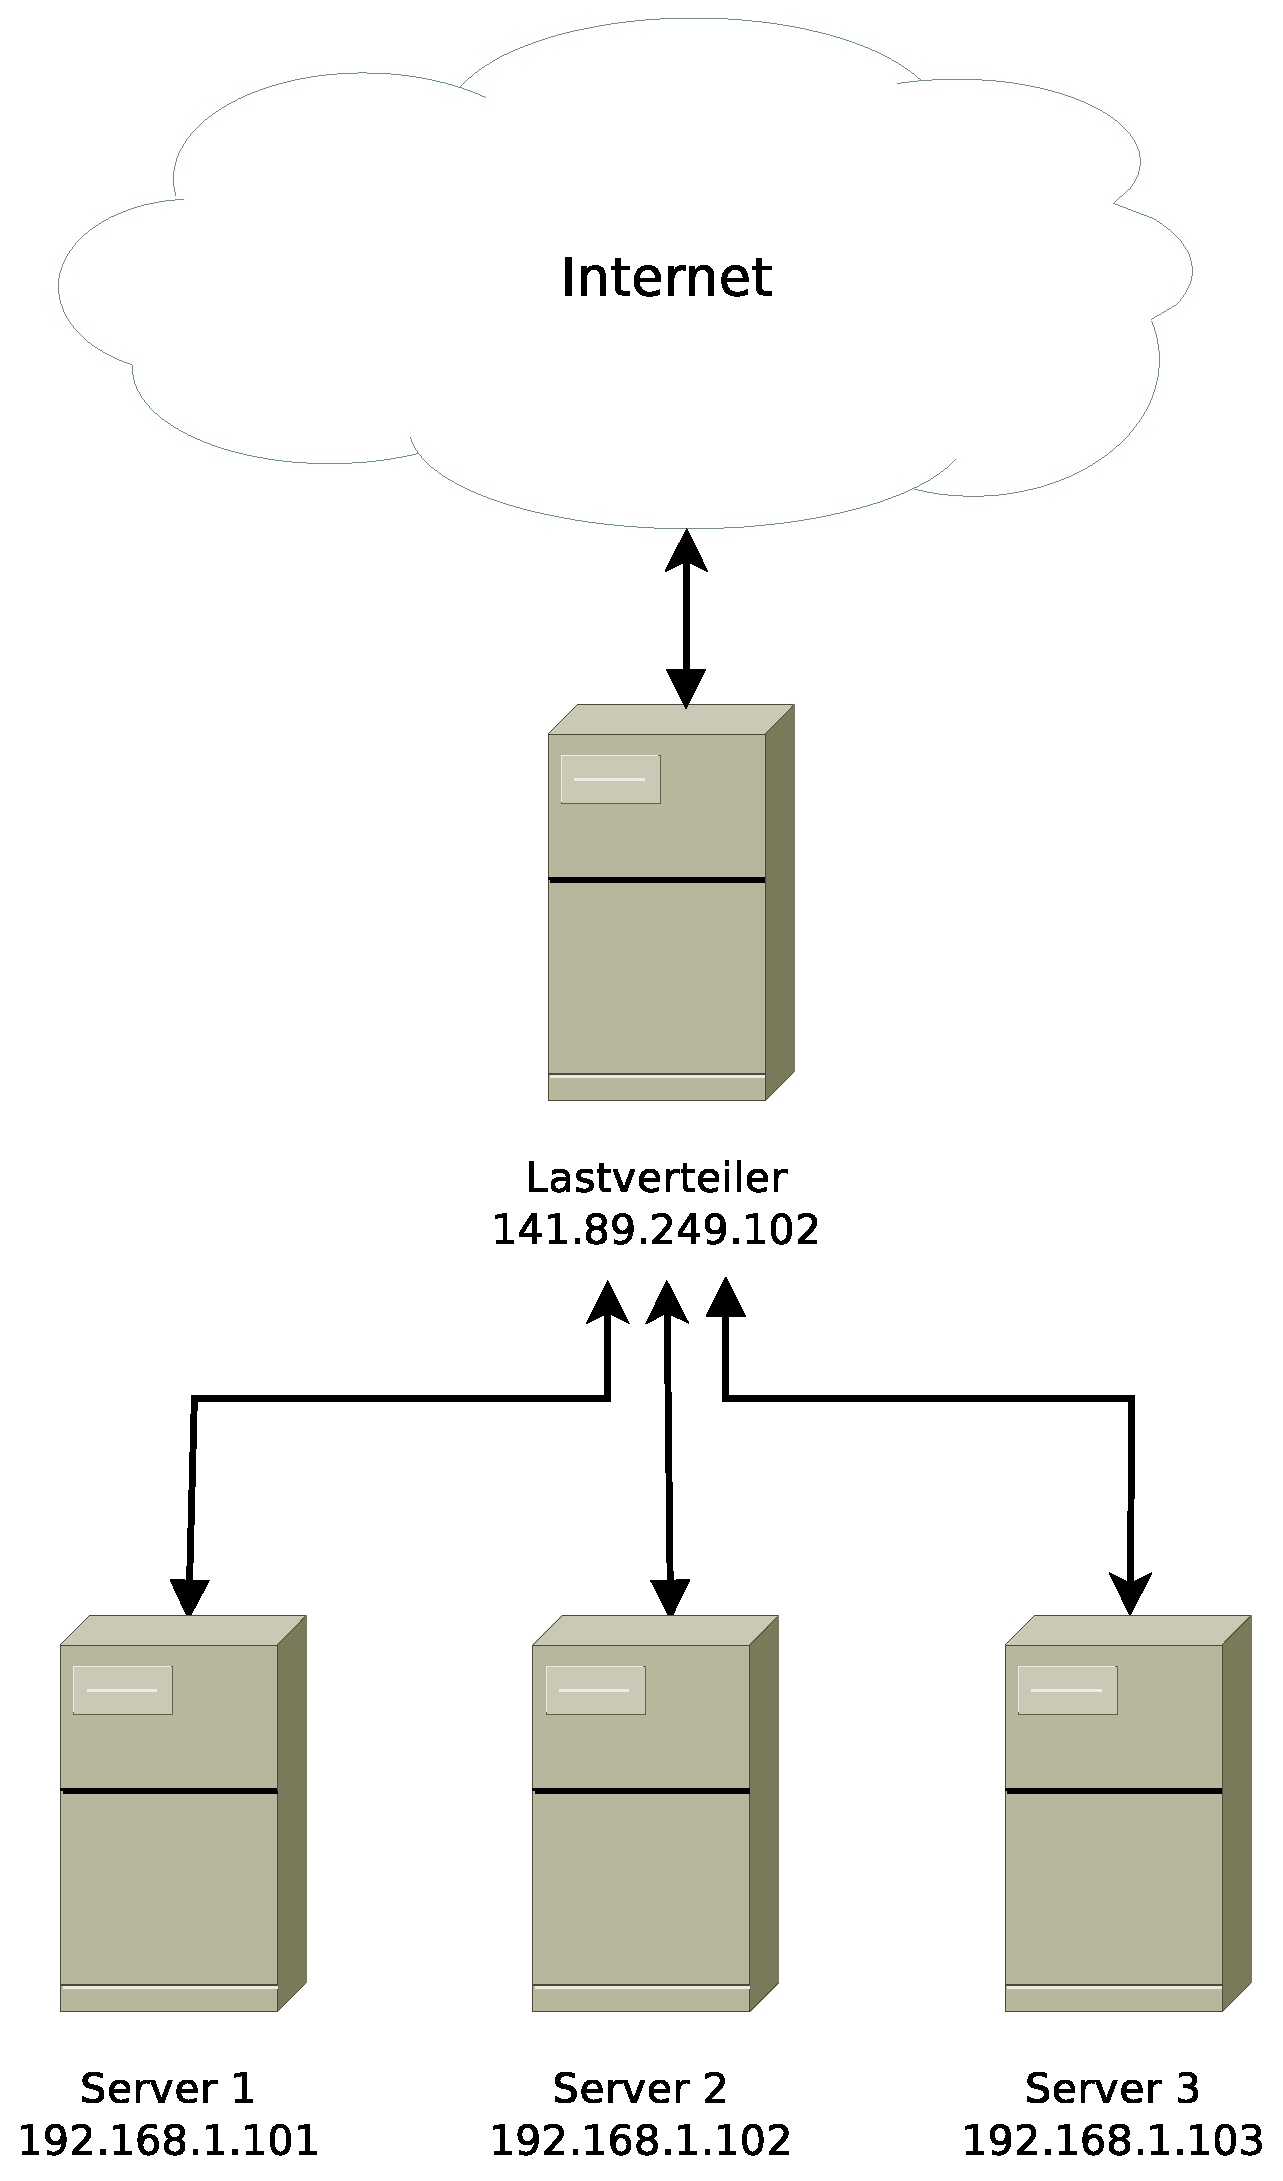
\includegraphics[width=\textwidth]{images/loadbalancer}
				\caption{Lastverteilung mit Hilfe eines Lastverteilers}
				\label{fig:loadbalancer}
			\end{figure}

			Bei dem Konzept der Server-Lastverteilung wird von der folgenden Situation ausgegangen.  Es
			existiert ein Cluster aus mehreren Servern, welche alle die selbe Anwendung (z.B. eine
			Website) zur Verfügung stellen. Diese sogenannten Backend-Server sind über einen
			Lastverteiler, einem weiteren Server, mit dem restlichen Netzwerk oder Internet verbunden
			(siehe Abbildung \ref{fig:loadbalancer}). Der Lastverteiler hat die folgenden Aufgaben
			\cite{bourke2001}:

			\begin{itemize}
				\item Entgegennehmen des kompletten Netzwerkverkehrs, welcher an die Anwendung gerichtet ist
					(z.B. HTTP-Anfragen an eine Website).
				\item Verteilung des angenommenen Netzwerkverkehrs auf die Backend-Server.
				\item Überwachung der Last der einzelnen Backend-Server und entsprechende Anpassung der
					Verteilung des Netzwerkverkehrs.
			\end{itemize}

			Diese Anforderungen können durch unterschiedliche Systeme realisiert werden. Ein Lastverteiler
			kann im Kernelspace oder Userspace des Betreibssystems
			implementiert sein. Ansätze für Userspace-basierte Lastverteiler sind zum Beispiel das Programm
			perlbal \cite{perlbal} oder das Apache-Modul mod\_proxy\_balancer \cite{modproxy}.  Eine
			Implementierung im Userspace hat den Vorteil, dass der Lastverteiler unabhängig von konkreten
			Betriebssystemen und Kernel-Versionen ist. Außerdem benötigt dieser keine \texttt{root}-Rechte
			um konfiguriert und gestartet zu werden. Da es sich um Anwendungen im Userspace handelt,
			findet hier die Lastverteilung auf einer höheren OSI-Schicht \cite{tanenbaum1988} statt.
			Dadurch stehen dem Lastverteiler anwendungsspezifischere Informationen zu einer Anfrage
			bereit. Dies kann dazu genutzt werden, die Abfragen nach deren Inhalt zu filtern
			und so ein kontextsensitives Verteilen zu ermöglichen.  Ein Nachteil, der vor allem bei
			hohem Netzwerkverkehr entsteht, ist der nötige Kontextwechsel, damit der Lastverteiler
			im Userspace die Netzwerkpakete auswerten kann. Dazu muss das Netzwerkpaket in den Userspace
			und zum Weiterversenden wiederum in den Kernelspace kopiert werden. Hierbei ist jeweils ein
			Kontextwechsel nötig, welcher bei hohem Netzwerkverkehr zu Leistungseinbußen führen kann
			\cite{boehme2006}.  Im Vergleich zu diesen Ansätzen im Userspace gibt es im Kernelspace den
			Linux Virtual Server (LVS) \cite{lvs,zhang2000} für Linux und den Paketfilter pf \cite{pf} für
			OpenBSD als bekannteste Beispiele.  Indem die Pakete bereits im Kernelspace verarbeitet
			werden, findet kein Kontextwechsel statt und die Verarbeitung kann schneller erfolgen.
			Allerdings findet die Verarbeitung auf einer der unteren Schichten des OSI-Modells statt, was
			dazu führt, dass keine anwendungsspezifischen Informationen vorliegen. Jedoch bietet dieser
			Ansatz eben genau dies auch als Vorteil, denn so kann eine Lastverteilung unabhängig von
			Anwendungen stattfinden.  Das heißt, ein Lastverteiler, wie der LVS, kann so konfiguriert
			werden, dass er gleichzeitig unterschiedlichen Netzwerkverkehr (z.B. unterschiedliche
			Transportprotokolle oder Portnummern) separat verteilt. Dies ist mit einer anwendungsbasierten
			Lösung nicht ohne weiteres realisierbar.

			Unabhängig von der gewählten Software-Lösung ist der gewählte Algorithmus zur Lastverteilung
			ein entscheidendes Kriterium. Es existieren mehrere Algorithmen für dieses Problem
			\cite{zinke2007}, wobei es von der gewählten Software abhängt, welche überhaupt zur Verfügung
			stehen.  Die zwei bekanntesten Verfahren sind das Round-Robin-Verfahren und das
			Least-Connection-Verfahren. Beim Round-Robin-Algorithmus wählt der Lastverteiler aus einer
			Liste von Servern den nächsten aus. Das geschieht zyklisch, was dazu führt, dass die
			Reihenfolge der Server immer gleich bleibt. Dies ist ein sehr einfacher Algorithmus der aber
			bei homogenen Clustern und homogenen Anfragen ausreicht, um die Last sinnvoll zu verteilen.
			Handelt es sich nicht um ein homogenes Cluster, so kann durch eine gewichtete Variante des
			Algorithmus die Last entsprechend der Leistung der Server verteilt werden. Sind jedoch die
			Anfragen an das Cluster nicht homogen, das heißt, jede Anfrage erzeugt eine unterschiedliche
			Last bei den Backend-Servern, kann das nicht durch den Round-Robin-Algorithmus ausgeglichen
			werden. Der zweite bekannte Algorithmus ist Least-Connection. Dieser Algorithmus beachtet bei
			der Verteilung die aktuelle Anzahl an Verbindungen zu den Backend-Servern. Arbeitet ein Server
			schneller seine Anfragen ab als ein anderer, erhält dieser Server früher wieder
			Anfragen. Auch von diesem Algorithmus gibt es eine gewichtete Variante, welche die bereits
			dynamisch getroffene Entscheidung noch einmal verbessern soll. Daher ist anzunehmen, dass
			Least-Connection bessere Ergebnisse auf heterogenen Clustern als Round-Robin erzielt und auch
			nicht homogene Anfragen begrenzt abfängt.

			% subsection Server-Lastverteilung }}}

			\subsection{DNS-basierte Lastverteilung} % {{{
			\label{sub:dns-lastverteilung}

			\begin{figure}
				\centering
				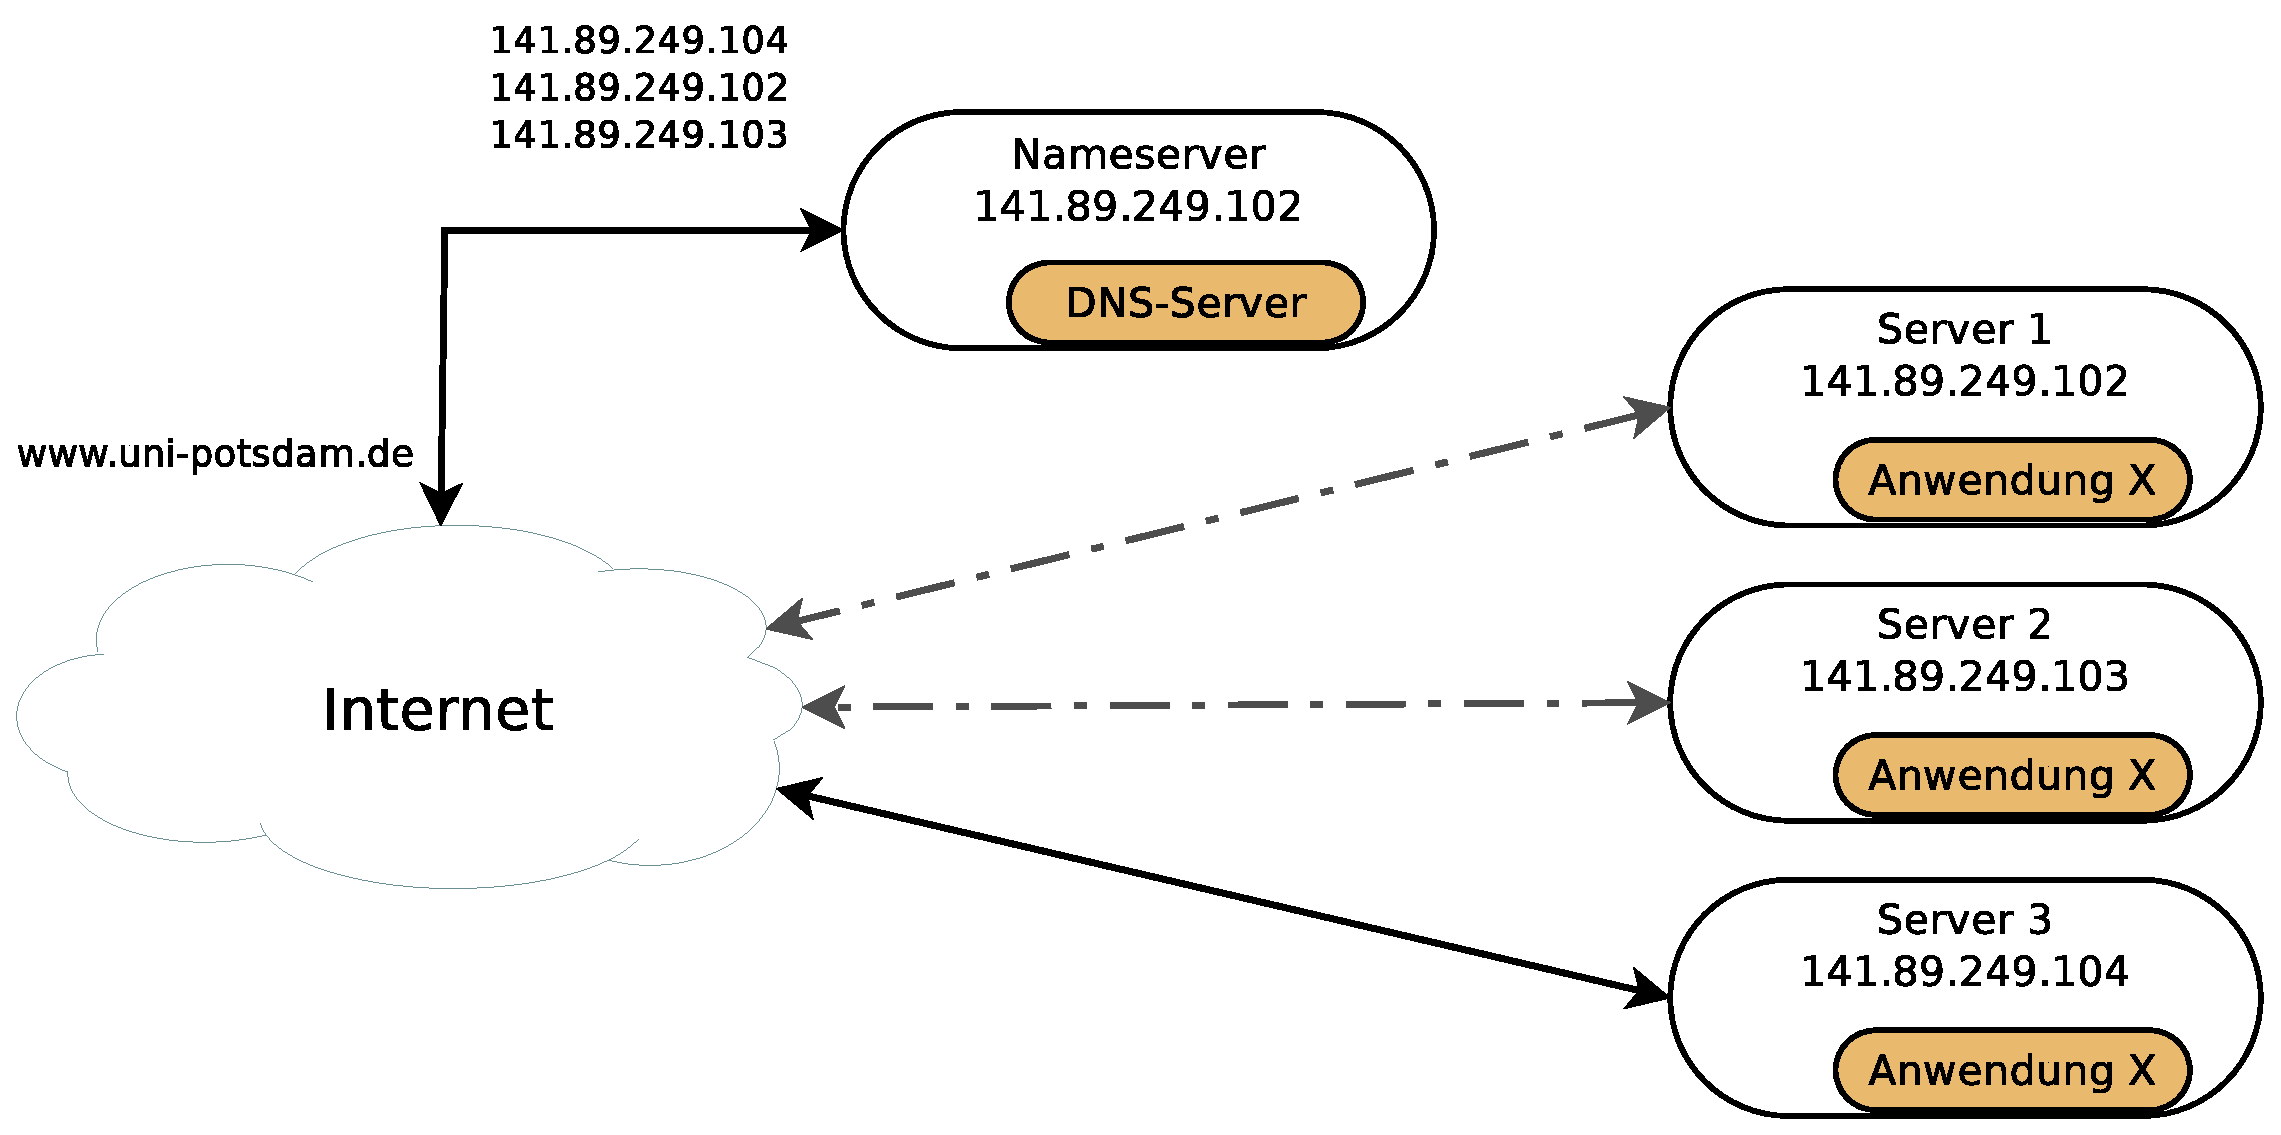
\includegraphics[width=12cm]{images/dns-loadbalancer}
				\caption{Lastverteilung mit Hilfe von DNS}
				\label{fig:lastverteilung-dns}
			\end{figure}

			Existiert kein Cluster oder soll auf einen zusätzlichen Server verzichtet werden, bietet sich
			eine DNS-basierte Lastverteilung an. Diese nutzt die Möglichkeit, dass einem DNS-Eintrag für
			eine Domain mehrere IP-Adressen zugeordnet werden können \cite{rfc1034}. Ein möglicher
			Verbindungsablauf ist in Abbildung \ref{fig:lastverteilung-dns} dargestellt. Hier wird als
			erstes der DNS-Server befragt, welcher dann eine Liste aller möglichen Adressen liefert. Dabei
			existiert keine Ordnung dieser Einträge und der DNS-Server entscheidet, in welcher Reihenfolge
			er die IP-Adressen zurückliefert. Oft wird dazu ein Round-Robin-Algorithmus genutzt und somit
			eine gewisse Lastverteilung erreicht. Dieses Verfahren hat jedoch einige Nachteile. So führt
			das Caching von lokalen Nameservern dazu, dass alle Anfragen zu derselben Adresse geleitet
			werden. Weiterhin hat der DNS-Server keine Informationen über die Last der Server oder
			darüber, ob diese überhaupt erreichbar sind. Dadurch wird ein Server, der ausgefallen ist,
			trotzdem immer wieder als Antwort zurückgeliefert. Es ist auch nicht möglich, Gewichte für die
			Verteilung der Last auf den Server anzugeben, weshalb eine Heterogenität der Server nicht
			ausgeglichen werden kann. Dieses Problem sollte durch den DNS-Typen \texttt{SRV}
			\cite{rfc2782} behoben werden.  Ein Beispiel eines \texttt{SRV}-Eintrags für einen Webserver
			ist in Tabelle \ref{tab:srv} zu sehen. Durch den Domain-Namen wird definiert, dass dieser
			Eintrag nur für HTTP-Anfragen über TCP an die Domain \texttt{bsp.de} gilt. In dem Beispiel
			wird anschließend den Domains \texttt{www.bsp.de} und \texttt{www2.bsp.de} eine Priorität von
			0 und \texttt{backup.bsp.de} von 1 zugeordnet. Dabei muss von einem Client der Server mit der
			kleinsten Priorität gewählt werden, sofern dieser erreichbar ist. Gibt es mehrere Server mit
			derselben Priorität (wie im Beispiel \texttt{www.bsp.de} und \texttt{www2.bsp.de}), sollte die
			Wahl eines Server mit einem höheren Gewicht wahrscheinlicher sein. Zusätzlich wird noch der
			Port für das Ziel angegeben.  Dieses Verfahren führt zwei Gewichtungen ein, welche auf der
			Client-Seite ausgewertet werden.  Allerdings ist die Unterstützung auf der Clientseite für
			\texttt{SRV}-Einträge sehr gering. Zusätzlich ergibt sich noch, dass der DNS-Server nicht die
			Last und Funktionstüchtigkeit der Server kennt.  Jedoch gibt es dem Client einen Anhaltspunkt,
			welchen Server er als nächstes kontaktieren sollte, sofern ein Server nicht erreichbar ist.

			\begin{table}
				\centering
				\begin{tabular}{|ccccccl|}\hline
				 Domain & Klasse & Typ & Priorität & Gewicht & Port & Ziel \\\hline\hline
					\_http.\_tcp.bsp.de. & IN & SRV & 0 & 2 & 80 & www.bsp.de. \\
					& IN & SRV & 0 & 1 & 80 & www2.bsp.de. \\
					& IN & SRV & 1 & 0 & 80 & backup.bsp.de. \\\hline
				\end{tabular}
				\caption{Beispiel für einen \texttt{SRV}-Eintrag für einen Webserver}
				\label{tab:srv}
			\end{table}

			Mit Geotargeting oder auch GeoIP genannt, ist es möglich, anhand der IP-Adresse eine Aussage
			über die ungefähre geografische Position des Inhabers zu treffen. Diese Information wird zum
			Beispiel beim Global Server Load Balancing (GSLB) \cite{bourke2001} verwendet, wodurch der
			DNS-Server seine Antwort an die geografische Position des Fragestellers anpassen kann. Der
			Gedanke dabei ist, dass ein geografisch naher Server auch der schnellere Server ist. Dies muss
			nicht immer der Fall sein und außerdem kann ist es möglich, dass der Client über einen DNS-Server
			Anfragen stellt, welcher selbst nicht geografisch nah ist. Dadurch kann es zu negativen
			Effekten kommen.

			Auch Kombinationen der Server-Lastverteilung und DNS-Lastverteilung sind möglich. Dabei wird ein
			DNS-Server um Lastverteilungsfunktionen erweitert. So beschreibt \cite{chyuyi2003} ein
			Verfahren, bei dem der DNS-Lastverteiler die Zeit überwacht, welche jeder Backend-Server für
			die Abfrage einer Antwort benötigt. Dadurch kann die DNS-Antwort entsprechend der
			Lastsitutation angepasst werden. Einen ähnlichen Ansatz findet man in \cite{mookim2005}. Dabei
			werden Backend-Server, die überlastet sind, aus der Round-Robin-Liste des DNS-Servers entfernt
			und dynamisch wieder hinzugefügt, sobald sie die Überlastsitutation überwunden haben.

			% subsection DNS-basierte Lastverteilung }}}

			\subsection{Lastverteilung von DNS-Verkehr} % {{{
			\label{sub:lastverteilung-dns}

			Die Verteilung von DNS-Anfragen unterscheidet sich in mehreren Punkten von HTTP-Anfragen. So
			ist das genutzte Transport-Protokoll UDP, statt TCP, und die Nachrichten dürfen nicht größer als
			\unit[512]{Byte} sein \cite{rfc1035}. Weiterhin existieren beim DNS keine Client-Sessions wie bei
			zustandsbehafteten HTTP-Anwendungen, wo ein Client während einer Session immer mit demselben Server
			kommunizieren muss. Die Lastverteilung von DNS-Anfragen tritt jedoch wesentlich seltener auf
			als bei HTTP-Anfragen. Firmen und Organisationen haben selten eine so hohe Anzahl an
			DNS-Anfragen, dass sie Überlastsituationen erreichen. Dies schließt nicht aus, dass mehrere
			DNS-Server existieren, welche aber oft nur als Schutz vor Ausfällen und anderen Störungen
			dienen.  In lokalen Netzwerken und kleinere Firmen reicht es daher aus, Lastverteilung mit Hilfe
			von DNS-Einträgen durchzuführen. Bei größeren Firmen, die eine höhere Anzahl an DNS-Anfragen
			zu bewältigen haben, ist der Einsatz eines DNS-Clusters und Server-Lastverteilers sinnvoll. Die
			größte Last liegt bei den Betreibern von TLDs und den Root-Servern. Für diese Anwendungsfälle
			sind DNS-Cluster nötig. Zusätzlich kommt Anycast \cite{rfc4786, sapate2005} zum Einsatz. Dabei
			werden mehrere DNS Server mit derselben Anycast-IP-Adresse mit dem Internet verbunden. Sendet
			nun ein Client eine Anfrage an diese Anycast-Adresse, antwortet der Server, der als erster die
			Frage erhält. Die Idee dabei ist, dass durch den DNS-Server, der die kürzeste Route zum
			Fragesteller hat, die beste Antwort gegeben werden kann. Vor allem bei den Root-Servern ist
			das sinnvoll. Es existieren insgesamt 13 Root-Server
			(A-M) \cite{rootserver}. Von ihnen nutzen 9 (A, C, F, G, I, J, K, L und M)
			Anycast-Adressen. Die anderen 4 Root-Server haben nur lokale Standorte in den USA.

			% subsection Lastverteilung von DNS-Verkehr }}}

		% section Lastverteilung }}}

		\section{Fazit} % {{{
		\label{sec:grundlagen-fazit}

			In diesem Kaptiel wurde die Enstehung und Bedeutung des \dns{} beschrieben. Es zeigt sich,
			dass die heutige Art der Nutzung des Internets ohne ein System, wie DNS, nicht möglich ist.
			Durch DNS wird eine schnelle und einfache Ermittlung von IP-Adressen realisiert. Infolgedessen
			muss das System jederzeit verfügbar sein und geringe Latenzen ermöglichen. Dafür werden die
			Informationen im DNS in einer verteilten Baumstruktur gespeichert. Diese ermöglicht das
			einfache Delegieren von Verantwortungen. Allerdings führt diese spezielle Struktur dazu, dass
			auf dem Wurzelknoten (Root-Domain) und seinen Kindknoten (TLDs) die größte Last liegt. Diese
			Last nimmt mit steigender Tiefe immer stärker ab. Folglich sind für die verschiedenen Ebenen
			des DNS jeweils andere Verfahren zur Lastverteilung geeignet. Es wurden die Konzepte der
			Server-Lastverteilung und DNS-basierten Lastverteilung vorgestellt.

			Um das verwendete System \textit{salbnet} in dieser Topologie einzuordnen, muss beachtet werden, dass
			\textit{salbnet} eine Server-Lastverteilung realisiert. Somit sind private Netzwerke und kleine
			Firmennetzwerke kein Anwendungsbereich für \textit{salbnet}. Bei Root-Servern, TLDs und großen SLDs ist
			es realistischer, dass DNS-Cluster genutzt werden, um die hohe Anzahl an DNS-Anfragen
			abzuarbeiten. Dementsprechend ordnet sich \textit{salbnet} bei solchen großen DNS-Systemen ein, bei denen
			der Einsatz eines DNS-Clusters unumgänglich ist und eine hohe Last entsteht.

			% Einordnung der Arbeit

		% section Fazit }}}

  % chapter Grundlagen }}}

	\chapter{Verwandte Arbeiten} % {{{
	\label{cha:arbeiten}

	Dieses Kapitel stellt verschiedene Arbeiten vor, welche sich hauptsächlich mit der Last von
	DNS-Root-Servern beschäftigen. Dabei soll gezeigt werden, welche Anzahl an Anfragen ein
	Root-Server erhält und von welcher Art diese sind. Zusätzlich soll auf Fehlverhalten innerhalb des
	DNS eingegangen werden und anhand von Anycast-Anfragen überprüft werden, ob es auch externe
	Effekte gibt, welche das DNS beeinflussen.

	Die Anfragen an ein DNS-Cluster des F-Root-Servers wurden Anfang 2001 in \cite{brclne2001}
	analysiert. Das Cluster bestand aus zwei DEC Alpha Systemen und einem Cisco-Router, welcher CEF
	(Cisco Express Forwarding) zur Lastverteilung nutzte. Die Untersuchung zeigt, dass es zu
	Lastspitzen mit bis zu 5000 Anfragen pro Sekunde kam und der Root-Server ca. \unit[93]{\%} der
	Anfragen sofort beantworten konnte. Die restlichen \unit[7]{\%} waren Anfragen, welche nicht
	beantwortet werden konnten, weil zum Beispiel die DNS-Anfragen falsch gestellt wurden. Sehr
	interessant sind die Ergebnisse bezüglich Nameserver bzw. Clients, welche nicht korrekt auf
	Antworten oder Fehler reagieren. So wurde ein Client im Log entdeckt, welcher 2.112.962 mal in
	einer Stunde dieselbe Anfrage stellte.  Insgesamt konnte festgestellt werden, dass in einem Log
	von 2 Stunden Dauer 29 Millionen Anfragen eingingen und davon \unit[85]{\%} wiederholte
	Anfragen waren (selber Client und selbe Anfrage). Außerdem wurden in einem Log von der Länge
	einer Stunde 143.783 verschiedene ungültige TLDs angefragt. Die Gründe für viele falsche Anfragen oder
	wiederholte Anfragen scheinen fehlerhafte Implementationen des DNS-Standards \cite{rfc1034,
	rfc1035} oder falsch konfigurierte Softwaresysteme zu sein. Diese fehlerhaften DNS-Anfragen
	machen ungefähr einen Anteil von \unit[14]{\%} aus. Außerdem werden Root-Server
	anscheinend oft für Denail of Service Angriffe genutzt. Dabei ist nicht der Root-Server das
	Ziel, sondern er wird als Reflektor verwendet und dabei werden eine große Menge an Anfragen mit
	veränderter Absenderadresse an ihn geschickt. Diese werden dann vom Root-Server beantwortet
	und an die falsche Absenderadresse, das Angriffsziel, gesendet. Dieses Zielsystem wird dadurch
	mit einer großen Menge an DNS-Antworten beschossen, obwohl es diese nie angefragt hat.

	Eine andere Art des Zusammenspiels von Schadsoftware und DNS wurde in \cite{isetal2005}
	untersucht.  Man beobachtete dazu das Verhalten eines Virus namens \glqq{}Antinny\grqq{} in Japan.
	Dieser Virus greift, vermutlich abhängig vom Wochentag, einen Webserver gezielt an. Um diesen
	Webserver mit Paketen zu beschießen und einen Denial of Service zu erreichen, benötigt der Virus
	die IP-Adresse des Ziels. Dazu stellt der Virus eine gewöhnliche DNS-Anfrage. Um die Anzahl dieser
	Anfragen zu messen, wurde der Nameserver des japanischen Internet Service Providers (ISP) Open
	Computer Networks (OCN) überwacht. Während einer Angriffsphase verzeichnete man durchschnittlich
	500 DNS-Anfragen pro Sekunde nach dem Zielsystem. Eine Entscheidung des Administrators des
	Webservers, welcher angegriffen wurde, zeigt die starken Abhängigkeiten innerhalb des DNS. Die
	Veränderung eines Eintrags im DNS kann schwerwiegende Folgen für andere Nameserver haben. So
	führte die Entfernung des DNS-Eintrags von dem angegriffenen Webserver dazu, dass der Virus den
	Domain-Namen nicht auflösen konnte. Die negative Antwort eines Nameservers hat ebenfalls eine
	Gültigkeitsdauer, und erst nach dieser sollte ein System erneut eine DNS-Anfrage für diesen
	Domain-Namen senden.  Allerdings kam es im Fall des Virus dazu, dass ein Großteil der infizierten
	Rechner nun wiederholt die Nameserver nach der IP-Adresse des Angriffsziels fragten. Dies wurde
	entweder durch den Virus beeinflusst, oder die Nutzer der infizierten Systeme hatten
	selbst die Konfiguration so angepasst, dass die Gültigkeitsdauer ignoriert wurde. Die Gründe dafür
	können verschiedener Art gewesen sein. Letztendlich führte dies dazu, dass allein bei dem
	Nameserver des Open Computer Networks bis zu 4500 Anfragen pro Sekunde nach dem Zielsystem
	eingingen. Dies stellt eine beachtliche zusätzliche Last für den Nameserver da. Diese hohe Last
	konnte erst wieder durch einen neuen DNS-Eintrag für das Zielsystem beendet werden. Dabei wurde
	jedoch nicht die richtige IP-Adresse zurückgeliefert, sondern eine Scheinadresse. Somit konnten
	alle Anfragen an die Scheinadresse von Routern herausgefiltert und verworfen werden.

	Eine zusätzlich Art der Verteilung von DNS-Anfragen sind Anycast-Adressen. Wie in
	\ref{cha:grundlagen} beschrieben, dienen sie dazu, dass ein Client eine Antwort von dem Nameserver
	erhält, welcher ihm am nächsten ist. Dies soll möglichst geringe Antwortzeiten generieren. In \cite{sapate2005}
	wird das Verhalten von Anycast-DNS-Servern Ende 2004 untersucht. Dazu werden die
	Root-Server F und K mit TLD-Servern von UltraDNS verglichen. Die Root-Server nutzen eine
	Anycast-Adresse für ihre verteilten Cluster, UltraDNS hingegen nutzt zwei Anycast-Adressen für
	alle ihre Server. Die Messungen zeigen, dass bei den Root-Servern nur \unit[15]{\%}-\unit[27]{\%}
	der Anfragen an den geografisch nächsten Cluster gesendet wurden. Im Vergleich dazu geschah dies bei
	UltraDNS sogar von \unit[45]{\%} bis \unit[53]{\%} der Anfragen. Allerdings zeigte sich, dass die
	DNS-Cluster der Root-Server eine höhere Erreichbarkeit hatten. Zusammenfassend
	ist zu sagen, dass Anycast eine sinnvolle Methode ist um DNS-Anfragen zu verteilen, aber stark von
	den Netzwerken und BGB-Routen abhängt. Somit können Netzwerkausfälle die Routen von Anycast-Anfragen stark
	beeinflussen.

	In \cite{lietal2007} wurde eine ähnlich Analyse der Anycast-Root-Server C, F und K untersucht mit Daten
	von Anfang 2006. Die Beobachtung fand über einen Zeitraum von 47,2 Stunden, annähernd 2 Tage,
	statt. Es konnte gezeigt werden, das der größte Teil der DNS-Server Anfragen von geografisch nahen
	Clients erhielt.  Allerdings gab es auch das Beispiel des F-Root-Server in Los Angeles, USA,
	welcher \unit[88]{\%} seiner Anfragen aus Asien erhielt. Ein zweites Beispiel ist der K-Root-Server
	nahe Delhi, Indien, dessen Anfragen zu über \unit[75]{\%} aus Nordamerika, Südamerika und Europa
	stammen. Hingegen waren die Anfragen vom K-Root-Server in Tokyo, Japan, zu \unit[99,7]{\%} aus
	Japan, wovon \unit[75]{\%} der Clients aus einer Entfernung unter \unit[1000]{km} kamen. Zusätzlich
	konnte gezeigt werden, dass in dem betrachteten Zeitraum die meisten Clients immer denselben
	DNS-Server befragten. So wechselten z.B. beim C-Root-Server nur \unit[1,7]{\%} der
	Clients den Nameserver. Bei dem F und K-Root-Server waren es \unit[1,4]{\%} bzw.
	\unit[4,7]{\%}.

	In Anbetracht der vorgestellten Ergebnisse ergibt sich, dass Lastverteilung, z.B. durch ein
	Cluster mit einem Lastverteiler, eine wichtige Komponente des DNS ist. Das gilt vor allem für
	Server, die sehr weit oben in der DNS-Hierarchie positioniert sind. Diese Systeme müssen jeder Zeit mit einem
	sprunghaften Anstieg an Anfragen rechnen. Dies kann durch fehlerhafte Systeme hervorgerufen werden,
	durch fahrlässige Veränderungen von Domain-Einträgen oder durch Schadsoftware und Angriffe. Die
	Verwendung von Anycast, als weitere Lastverteilungsebene, scheint sich besonders für
	DNS-Root-Server zu eigenen. Die präsentierten Ergebnisse zeigten alle einen positiven Einfluss von
	Anycast-Servern. Allerdings wird durch dieses Verfahren das DNS System auch anfällig für externe
	Störungen. Dabei ist vor allem das BGB-Protokoll als Problem zu nennen, falsche oder ungünstige
	Routen haben einen starken Einfluss auf die Antwortzeiten von Anycast-DNS. Dennoch ist die lokale
	Lastverteilung in einem Cluster aus DNS-Servern entscheidend für die Stabilität und Zuverlässigkeit
	des DNS. Aus diesem Grund hat die hier entwickelte selbst-adaptive Lastverteilung für DNS-Anfragen, bzw.
	UDP-Anfragen im Allgemeinen, einen klaren Anwendungsfall in der Realität des DNS.

	% chapter Verwandte Arbeiten }}}

	\chapter{salbnet} % {{{
	\label{cha:salbnet}

		Dieses Kapitel beschreibt \textit{salbnet} \cite{salbnet}, einen Credit-basierten
		Lastverteilungsansatz.  Er basiert auf Arbeiten zur selbst-adaptiven Lastverteilung von
		TCP-Verkehr vor allem in InfiniBand-Netzwerken \cite{zinke2007, scsczile2008,
		schneidenbach2009}. Die Besonderheit an diesem Lastverteilungsverfahren ist, dass es sowohl eine
		Komponente auf dem Lastverteiler als auch auf den Backend-Servern gibt. Dabei werden auf den
		Backend-Servern Credits bestimmt, welche die Verfügbarkeit des Servers wiederspiegeln sollen,
		und an den Lastverteiler übermittelt. Der Lastverteiler wählt dann anhand der gemeldeten
		Credits die Backend-Server aus. Dieser Aufbau von \textit{salbnet} ist in Abbildung \ref{fig:salbnet} zu
		sehen, wobei die Komponenten von \textit{salbnet} blau hervorgehoben sind. Sie sollen im Folgenden kurz
		vorgestellt werden.

		\begin{figure}
			\centering
			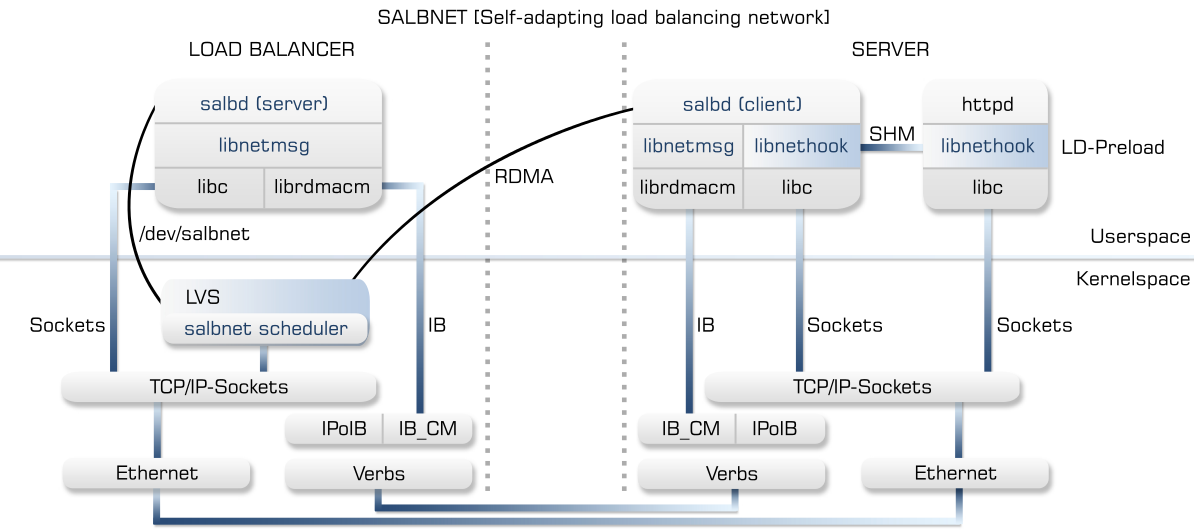
\includegraphics[width=\textwidth]{images/salbnet.png}
			\caption{Aufbau von \textit{salbnet} (übernommen aus \cite{zinke2012})}
			\label{fig:salbnet}
		\end{figure}

		\subsection*{libnetmsg} % {{{

			Die \textit{libnetmsg} \cite{rabweg2009} ist eine leichtgewichtige Kommunikations-Bibliothek die zur
			Übertragung sowohl UDP und TCP als auch InfiniBand unterstützt. Außerdem kann bei InfiniBand
			die Remote Direct Memory Access (RDMA) Eigenschaft genutzt werden. In \textit{salbnet} wird die
			Bibliothek eingesetzt um die Credits von den Backend-Server an den Lastverteiler zu melden. Wird
			InfiniBand verwendet können die neuen Credits mit Hilfe von RDMA direkt in den Kernelspeicher
			des Lastverteilers geschrieben werden. Dieses Vorgehen ist in Abbildung \ref{fig:salbnet}
			dargestellt.

		% subsection libnetmsg }}}

		\subsection*{libnethook} % {{{

			Mit der dynamischen Bibliothek \textit{libnethook} können Funktionsaufrufe von Anwendungen überwacht
			werden. So kann ermittelt werden wie oft eine Funktion aufgerufen bzw. was von ihr
			zurückgegeben wird. Im Fall von \textit{salbnet}, wird der \texttt{accept}-Funktionsaufruf vom Apache
			Webserver (httpd) \cite{httpd} abgefangen und analysiert. In Abbildung \ref{fig:salbnet} ist
			angedeutet, dass \textit{libnethook} zwischen dem httpd und der \textit{libc} agiert. Allgemein kann das auch
			für alle anderen TCP-Anwendungen instrumentalisiert werden. Im TCP-Fall wird nur die Anzahl
			der Funktionsaufrufe gezählt, um eine Neuberechnung der Credits auszulösen.

		% subsection libnethook }}}

		\subsection*{salbd} % {{{

			Die Hauptkomponente von \textit{salbnet} ist \textit{salbd}, welches sowohl auf dem Backend-Server als auch auf
			dem Lastverteiler zum Einsatz kommt. Auf dem Lastverteiler stellt \textit{salbd} einmal ein Kernelmodul
			bereit, das den \textit{salbnet} Scheduler für LVS implementiert. Dieser wählt Round-Robin den
			nächsten Backend-Server aus allen Servern, welche noch Credits größer 0 besitzen, aus. Außerdem
			wird \textit{salbd} genutzt, um Credits von Backend-Servern zu empfangen und bei Übertragungen
			ohne RDMA, auch um die Credits in den Kernelspace zum \textit{salbnet} Scheduler zu übermitteln.  Im
			Backend ist \textit{salbd} zur Bestimmung der Credits anhand der aktuellen Last der Webserver
			verantwortlich. Dazu werden verschiedene Metriken verwendet und anhand der ermittelten Werte
			verschiedene Meldestrategien verfolgt. Dieser Ablauf ist schematisch in Abbildung
			\ref{fig:salbd} dargestellt. Dabei überwacht \textit{salbd} die ensprechende Anwendung (z.B.
			httpd) und ermittelt dadurch Metriken, welche genutzt werden, um Credits zu berechnen. Diese
			werden dann zum Lastverteiler übermittelt.

		% subsection salbd }}}

		\begin{figure}
			\centering
			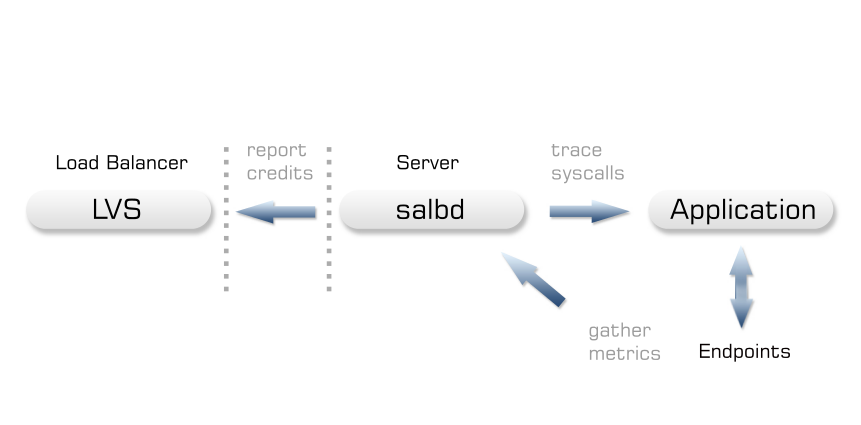
\includegraphics[width=\textwidth]{images/salbd-concept.png}
			\caption{Konzept von \textit{salbd} (übernommen aus \cite{zinke2012})}
			\label{fig:salbd}
		\end{figure}

		\section{Metrik und Credits} % {{{
		\label{sec:metrik}

			In \cite{zinke2012} werden die Forschungsergebnisse über \textit{salbnet} vorgestellt.  Dabei ist die
			Idee von \textit{salbnet} Credits zur Bewertung von Lastsitutationen zu nutzen. Das bedeutet, dass die
			Backend-Server ihre aktuelle Last ermitteln und daraus eine Credit-Anzahl bestimmen. Diese
			soll der Anzahl von Anfragen entsprechen, welche zum aktuellen Zeitpunkt zusätzlich vom Server
			abgearbeitet werden könnten. Diese Anzahl an Credits werden dem Lastverteiler gemeldet. Der
			Lastverteiler entscheidet mit einem einfachen Round-Robin-Verfahren, welcher Server die
			nächste Anfrage erhält.  Dazu werden alle Server, welche noch Credits besitzen, durchiteriert.
			Wird eine Anfrage einem Server zugewiesen, werden dessen Credits um eins verringert. Fallen
			die Credits eines Servers auf 0 und sendet er keine neuen Credits, wird er aus der Liste der
			verfügbaren Server entfernt. Meldet ein entfernter Server, erneut Credits, wird er wieder in
			die Verteilung aufgenommen. Die beiden wichtigsten Komponenten dieses Algorithmus sind die
			Metrik zur Berechnung der Credits und die Meldestrategie der Backend-Server.

			Die Metrik hat folgende Anforderungen zu erfüllen \cite{scsczile2008}:

			\begin{itemize}
				\item Sie sollte einfach zu berechnen sein.
				\item Sie sollte die aktuell zur Verfügung stehenden Ressourcen des Servers angeben.
				\item Sie sollte applikationsunabhängig sein.
				\item Sie sollte auch für Dienste mit mehreren Tausend Clients skalieren.
			\end{itemize}

			Die Version von \textit{salbnet} vor dieser Arbeit war auf TCP-Anfragen begrenzt. Dazu wurde eine
			Metrik beruhend auf der TCP-Backlog des Webservers entwickelt. Die Backlog erfüllt alle
			gestellten Anforderungen an eine gute Metrik. Sie ist einfach zu berechnen, da der aktuelle
			Füllstand und der maximale Füllstand leicht abfragbar sind. Die Backlog des Webservers
			entspricht einer Warteschlange für den Server. Solange die Backlog leer ist, kann der
			Webserver alle Anfragen sofort beantworten. Wenn die Anfragen in der Backlog gespeichert
			werden, ist der Server nicht mehr zu einer sofortigen Abarbeitung in der Lage. Die wartenden
			Anfragen werden nun in der Backlog gespeichert. Das heißt, die Anzahl der noch freien Plätze
			in der Backlog gibt die Anzahl der noch möglichen Verbindungen an. Ist die Backlog voll und es
			treffen weitere Anfragen ein, werden diese verworfen.  Somit kann die Anfrage nicht
			beantwortet werden.  Daher entspricht der aktuelle Füllstand der Backlog genau den aktuell zur
			Verfügung stehenden Ressourcen des Servers. Dadurch, dass die TCP-Backlog überwacht wird, ist
			diese Methode allgemein für alle Webserver nutzbar und somit applikationsunabhängig. Außerdem
			benötigt die Metrik keine besonderen Ressourcen, das heißt, sie ist weder Speicher- noch
			CPU-intensiv, und somit beeinflusst sie die Leistung des Webservers nicht.

			Die Betrachtung der Backlog zeigt auch zwei wichtige Metriken zur Bewertung einer Lastverteilung
			für Webserver. Das Verwerfen einer Anfrage muss mit allen Möglichkeiten verhindert werden. Jede
			verworfene Anfrage kann einem verlorenen Nutzer oder Kunden entsprechen. Muss eine Anfrage sehr
			lange in der Backlog warten, ist dies zwar nicht so ungünstig, wie eine verworfene Anfrage, aber
			es bedeutet eine längere Wartezeit für den Nutzer. Wenn dieser nicht bereit ist, so lange auf eine
			Antwort zu warten, hat man einen Nutzer oder Kunde verloren. Das heißt, eine gute
			Lastverteilung sollte zu einer geringen Zahl an verworfenen Anfragen und einer minimalen
			Antwortzeit führen.

		% section Metrik und Credits }}}

		\section{Meldestrategien} % {{{
		\label{sec:meldestrategien}

			Als zweiter wichtiger Faktor des Credit-Ansatzes zählt neben der Metrik die Meldestrategie. Dabei
			ist es entscheident, wieviele und wie oft Credits gemeldet werden. Eine häufige Meldung von Credits
			könnte eine zusätzliche Last auf den Backend-Servern erzeugen. Werden Credits zu selten
			gemeldet,
			kann es sein, dass der Backend-Server beim Lastverteiler aussortiert wird, weil seine Credits auf
			0 gefallen sind. Folgend werden 4 mögliche Meldestrategien vorgestellt \cite{scsczile2008, schneidenbach2009}.

			\paragraph{Plain} % {{{
			\label{par:plain}

				Plain stellt die einfachste Lösung vor. Dabei wird immer nach einem fixen Intervall die
				Differenz zwischen der maximalen Größe der Backlog und dem aktuellen Füllstand der Backlog
				gemeldet. Dies entspricht allen aktuell verfügbaren Ressourcen.

			% paragraph Plain }}}

			\paragraph{Soft + Hard Credits} % {{{
			\label{par:soft-hard-credits}

			Bei diesem Algorithmus werden dem Lastverteiler zweimal Credits mitgeteilt. Die Hard-Credits
			entsprechen den aktuell verfügbaren Ressourcen wie schon beim Plain-Algorithmus. Die Soft-Credits
			sind eine Empfehlung vom Backend-Server an den Lastverteiler. Sie ergeben sich aus den
			Hard-Credits und der aktuellen Lastsitutation, das heißt, wenn der Server Probleme hat die Backlog
			abzuarbeiten, sinken die Soft-Credits. Somit soll verhindert werden, dass zu viele Requests an den
			schon unter Last stehenden Server gesendet werden. Für den Lastverteiler sind grundsätzlich die
			Soft-Credits das ausschlaggebende Maß. Erst, wenn kein Server mehr über Soft-Credits verfügt,
			werden die Hard-Credits beachtet.

			% paragraph Soft + Hard Credits }}}

			\paragraph{Dynamic Report} % {{{
			\label{par:dynamic-report}

			Dynamic Report ersetzt das feste Meldeintervall des vorherigen Algorithmus durch ein dynamisch
			berechnetes. Dabei bildet ein festes Intervall eine Untergrenze. Dies verhindert eine Meldung nach
			jeder abgearbeitet Anfrage. Dieser Algorithmus meldet oft Credits, wenn die Backlog nur leicht
			gefüllt ist und eine geringe Last auf dem Server liegt. Ist die Backlog stark gefüllt und der
			Server mit der Abarbeitung der Anfragen beschäftigt, werden die Credits seltener gemeldet. Das
			führt dazu, dass bei vielen Anfragen keine zusätzliche Last durch unnötige Credit-Meldungen entsteht
			und bei geringer Last der Lastverteiler immer aktuelle Werte vom Backend-Server besitzt.

			% paragraph Dynamic Report }}}

			\paragraph{Dynamic Pressure Relieve} % {{{
			\label{par:dynamic-pressure-relieve}

			Der Dynamic Pressure Relive Algorithmus kombiniert alle vorherigen Algorithmen. Es existieren
			wiederum Hard- und Soft-Credits. Allerdings werden die Hard-Credits spätestens nach einem
			fixen Intervall und die Soft-Credits nach dem dynamischen Intervall aus dem Dynamic Report
			Algorithmus gemeldet. Bei einer Meldung der Soft-Credits an den Lastverteiler werden
			gleichzeitig die Hard-Credits mitgesendet. Dieses Vorgehen soll verhindern, dass zu selten
			Hard-Credits bei hoher Last gemeldet werden, was zu einer unnötig hohen Anzahl an verworfenen
			Anfragen führen kann.

			% paragraph Dynamic Pressure Relieve }}}

			Bei einer Simulation der verschiedenen Meldestrategien hat der Dynamic Pressure Relieve
			Algorithmus die besten Ergebnisse erzielt \cite{scsczile2008}.

		% section Meldestrategien }}}

		\section{Benchmark} % {{{
		\label{sec:Benchmark}

			Um \textit{salbnet} auf Webclustern zu testen, wurde der Benchmark servprep/servload
			\cite{habenschuss2011} entwickelt. Dabei ist servprep ein Programm, welches Logs des Apache
			Webservers einliest und diese modifizieren kann. So können alle Anfragen vervielfacht,
			Spitzenlasten verstärkt oder über einen Bewertungsalgorithmus neue Anfragen eingefügt werden,
			welche die Charakteristik des Log-Verlaufs nicht verändern. Die servload Anwendung ist der
			eigentliche Benchmark, der das von servprep vorbereitete Log wieder einspielt. Dabei ist
			servprep in der Programmiersprache Lua und servload in C geschrieben. In der weiteren
			Entwicklung des Benchmarks wurde servprep in servload integriert. Dadurch konnte eine noch
			bessere Leistung erzielt und der Ressourcenverbrauch minimiert werden. In \cite{menski2012}
			wurde servload in sofern erweitert, dass es Logs vom BIND DNS-Server verarbeiten und
			DNS-Anfragen über UDP versenden kann. Somit ist es möglich, servload in dieser Arbeit als
			Benchmark einzusetzen.

		% section Benchmark }}}

		\section{Fazit} % {{{
		\label{sec:salbnet-fazit}

			In diesem Kapitel wurden die theoretischen Grundlagen und der Aufbau von \textit{salbnet} erläutert.
			Der selbst-adaptive Lastverteiler \textit{salbnet} besteht aus den Komponenten \textit{libnetmsg}, \textit{libnethook}
			und \textit{salbd}. Hierbei ist \textit{salbd} die Hauptkomponente und stellt ein Kernelmodul für den LVS
			bereit, sowie eine Client-Komponente, welche die Credits auf den Backend-Servern berechnet.
			Zusätzlich wurden die bereits implementierten Metriken und Meldestrategien von \textit{salbnet}
			erläutert. Dabei handelt es sich um die TCP-Backlog-Metrik für TCP-Anfragen. Von den
			vorhandenen Meldestrategien ist vor allem der Dynamic Pressure Relieve Algorithmus zu
			erwähnen. Dieser konnte bereits in Simulationen und Tests überzeugen.

			Zusätzlich zum \textit{salbnet} wurde der Benchmark servload entwickelt, welcher in
			\cite{menski2012} erweitert wurde, um DNS-Anfragen zu unterstützen. Dieser
			Benchmark bietet sich vor allem deshalb an, weil es mit ihm möglich ist, aus realen
			BIND-Logs eine hohe Last zu generieren, indem diese durch verschiedene Algorithmen
			verstärkt werden. Weiterhin sind auch die ausführlichen Statistiken, welche vom
			servload-Benchmarks generiert werden, ein wichtiger Grund für die Wahl.

			Basierend auf diesen Informationen wird im folgenden Kapitel ein Konzept dafür erarbeitet, wie
			sich \textit{salbnet} auf DNS-Anfragen anpassen lässt.  Dessen Umsetzung im Folgenden mit dem
			servload-Benchmark getestet wird.

		% section Fazit }}}

	% chapter salbnet }}}

	\chapter{Konzept} % {{{
	\label{cha:konzept}

	In diesem Kapitel sollen mögliche Konzepte zur Erweiterung von \textit{salbnet} für DNS-Anfragen
	vorgestellt werden. Anschließend wird eines der Konzepte ausgewählt und ein Entwurf zur Implementierung
	präsentiert. Die Implementierung des gewählten Entwurfs wird dann in Kapitel
	\ref{cha:implementierung} beschrieben.

		\section{Ansätze} % {{{
		\label{sec:ansaetze}

		Wie in Kapitel \ref{cha:salbnet} beschrieben, ist \textit{salbnet} ursprünglich nur für TCP-Anwendungen
		konzipiert und für den Apache Webserver implementiert. Dazu wurde eine Metrik über die Backlog
		des TCP-Sockets des Webservers erstellt. Diese gibt die konkrete Anzahl der Anfragen an, welche
		noch in der Backlog Platz finden würden. Das heißt, es sollten nicht mehr als diese Anzahl von
		Anfragen an den Server gestellt werden, sonst existiert die Gefahr, dass die Anfragen verworfen
		werden. Aufgabe dieses Kapitels ist es, verschiedene Ansätze zu beschreiben, welche eine ähnlich
		gute Metrik für UDP-Anfragen erzeugen.

		\subsection*{Last-Metrik} % {{{

		Wenn sich ein Server in einer Überlastsitutation befindet, erkennt man das oft daran, dass
		bestimmte Ressourcen aufgebraucht sind. So kann eine \unit[100]{\%}ige CPU- oder RAM-Auslastung aussagen,
		dass der Server an seine Grenzen geraten ist. Daher ist eine mögliche Metrik die Sammlung
		entsprechender Last-Daten und eine anschließende Abschätzung bezüglich der verbleibenden
		Ressourcen.

		% subsection Last-Metrik }}}

		\subsection*{Verkehr-Metrik} % {{{

		Bei Servern, die einen Dienst für das Netzwerk bereitstellen, kann das Verhältnis der
		eingehenden und ausgehenden Nachrichten eine mögliche Metrik für die Lastsitutation des Servers
		darstellen.  Ein Server, der alle eingehenden Nachrichten sofort beantworten kann, und somit die
		gleiche Anzahl an ausgehenden Nachrichten erzeugt, befindet sich in keiner Überlastsituation.
		Hat der Server jedoch Probleme, eingehende Anfragen direkt zu beantworten, befindet er sich
		unter einer gewissen Last, bis hin zur Überlast, bei der Anfragen verworfen werden müssen. Um
		die Lastsitutation zu untersuchen ist es möglich, die Anzahl der eingehenden und abgearbeiteten
		(ausgehenden) Anfragen zu protokollieren. Wenn die Differenz nahe 0 ist, geht man von keiner
		hohen Last aus.  Wächst die Differenz jedoch allmählich, befindet sich der Server unter
		steigender Last.

		% subsection Verkehr-Metrik }}}

		\subsection*{Receive-Queue-Metrik} % {{{

		Ein Ansatz ähnlich des TCP-Backlog-Ansatzes \cite{zinke2007,scsczile2008} ist das Überwachen
		der Receive-Queue des UDP-Sockets des DNS-Servers. Anders als bei dem TCP-Fall werden in
		der Receive-Queue keine Verbindungen verwaltet, sondern Pakete unterschiedlicher Größe
		gespeichert. Das heißt, die Receive-Queue hat eine maximale Größe und ist bis zu einem
		bestimmten Punkt gefüllt. Dies sagt aber nichts über die Anzahl an Paketen in der Receive-Queue
		aus.  Trotzdem könnte eine Metrik darin bestehen, den verbleibenden Platz in der Receive-Queue
		zu bestimmen, um daraus eine Abschätzung zu treffen, wieviele weitere Anfragen aufgenommen
		werden könnten.

		% subsection Receive-Queue-Metrik }}}

		% section Ansätze }}}

		\section{Auswahl} % {{{
		\label{sec:auswahl}

		Nachdem in Abschnitt \ref{sec:ansaetze} mehrere Ansätze vorgestellt wurden, sollen diese nun
		bewertet werden. Danach wird ein Ansatz ausgewählt, welcher dann weiter verfeinert wird. Die
		Bewertung der Ansätze erfolgt nach den in Kapitel \ref{cha:salbnet} aufgeführten Anforderungen
		an eine Metrik, welche waren:

		\begin{itemize}
			\item Sie sollte einfach zu berechnen sein.
			\item Sie sollte die aktuell zur Verfügung stehenden Ressourcen des Servers angeben.
			\item Sie sollte applikationsunabhängig sein.
			\item Sie sollte auch für Dienste mit mehreren Tausend Clients skalieren.
		\end{itemize}

		\subsection*{Last-Metrik} % {{{

		Die Last-Metrik ist applikationsunabhängig und wird auch nicht durch die Anzahl der Clients
		beeinflusst. Allerdings ist es schwer, aus Faktoren wie der CPU-Last, RAM-Auslastung, Load etc.
		eines Servers Aussagen über die aktuelle Lastsituation des Servers zu treffen. In
		\cite{kunz1991} wurden verschiedene Last-Metriken untersucht. Dabei wurde gezeigt, dass einfache
		Metriken bessere Ergebnisse lieferten als mehrdimensionale, über mehrere Indizes. Die
		besten Ergebnisse wurden mit einer Metrik, die sich ausschließlich auf die Länge der
		CPU-Warteschlange bezieht, erzielt. Bei dieser Untersuchung wurde ausschließlich ein homogenes System
		betrachtet. Um diese Metriken auf ein heterogenes System anzuwenden, muss eine Normierung
		vorgenommen werden, damit die Systeme und deren Metriken vergleichbar werden. Dazu schlägt
		\cite{lansch1994} die Formel \ref{eq:load} vor, bei der $\alpha$ eine Architekturkonstante für
		die Grundgeschwindigkeit und \textit{load} die aktuelle Last des Systems ist.

		\begin{equation}
			I := \alpha \cdot (1 + \text{load})
			\label{eq:load}
		\end{equation}

		Selbst, wenn eine normierte Metrik genutzt wird, existiert dennoch das Problem, dass mit dieser
		Metrik eine Abschätzung über die noch möglichen Ressourcen, in Form von weiteren Anfragen, nicht
		einfach ist. Zum Beispiel lässt sich kaum aus der Länge der CPU-Warteschlange abschätzen,
		wieviel weitere Anfragen der Server noch empfangen kann, bevor er in eine Überlastsituation
		gerät. Aus diesem Grund ist die Metrik schwer zu berechnen, bzw. führt nur zu sehr ungenauen
		Abschätzungen und erfüllt damit nicht die Anforderungen.

		% subsection Last-Metrik }}}

		\subsection*{Verkehr-Metrik} % {{{

		Die Verkehr-Metrik ist ebenfalls applikationsunabhängig und einfach zu berechnen, da nur die
		Differenz der eingehenden und ausgehenden Anfragen ermittelt werden muss. Ist diese Differenz
		negativ, ist der Server schneller im Abarbeiten als dass neue Anfragen eintreffen. Ist sie
		gleich 0, ist der Server in einem Gleichgewicht, in dem er alle eintreffenden Anfragen sofort
		beantworten kann.  Ist die Differenz positiv, stauen sich Anfragen beim Server. Steigt diese
		Differenz immer weiter an, kann davon ausgegangen werden, dass der Server Probleme hat, weitere
		Anfragen abzuarbeiten. Die Probleme dieser Metrik sind jedoch die Abbildung der Differenz auf
		die verfügbaren Ressourcen des Servers. Das bedeutet, es ist schwer, anhand der Differenz auf
		die noch möglichen Anfragen zu schließen, welche der Server zusätzlich abarbeiten könnte, ohne
		dass eine Anfrage verworfen wird. Es könnte eine Abschätzung der maximal möglichen Anfragen pro
		Zeitintervall genutzt werden. Diese vernachlässigt allerdings die UDP-Eigenschaft, dass in der
		Receive-Queue keine Anfragen sondern Pakete gespeichert werden. Das heißt, die maximale Anzahl
		an Anfragen pro Zeitintervall hängt von den einzelnen Paketgrößen ab. Außerdem kann davon
		ausgegangen werden, dass ein Protokollieren aller ein- und ausgehenden Anfragen nicht gut
		skaliert. So würde bei einer hohen Anzahl von Anfragen an den Server die Überwachung eine
		zusätzlich Last erzeugen, welche den Server darüber hinaus belastet. Folglich erfüllt auch diese
		Metrik ebenfalls nicht die Anforderungen.

		% subsection Verkehr-Metrik }}}

		\subsection*{Receive-Queue-Metrik} % {{{

		Die Receive-Queue-Metrik ist, wie auch die beiden vorherigen, applikationsunabhängig, da sie
		sich auf die Receive-Queue des UDP-Sockets bezieht. Sie erzeugt auch keine zusätzliche Last,
		wenn die Client-Anzahl steigt. Die Berechnung ist etwas schwieriger als bei der
		TCP-Backlog-Metrik, da, wie bereits erwähnt, keine Verbindungen gespeichert werden, sondern
		Pakete. Allerdings kann aus dem verbleibenden Platz in der Receive-Queue und einer Abschätzung
		über die durchschnittliche Paketgröße eine Vorhersage getroffen werden, welche zusätzliche
		Anzahl an Anfragen der Server verarbeiten könnte. Damit erfüllt die Metrik auch die
		Anforderungen der einfachen Berechnung und der Angabe von verfügbaren Ressourcen.

		% subsection Receive-Queue-Metrik }}}

		Wie bereits durch die vorhergehenden Bewertungen zu erkennen ist, hat nur die Receive-Queue-Metrik die
		Anforderung aus \cite{scsczile2008} an eine Metrik für \textit{salbnet} erfüllt. Diese wird in Abschnitt
		\ref{sec:entwurf} genauer beschrieben und in Kapitel \ref{cha:implementierung} wird die
		konkrete Implementierung in \textit{salbnet} erläutert.

		% section Auswahl }}}

		\section{Entwurf} % {{{
		\label{sec:entwurf}

		Die ausgewählte Receive-Queue-Metrik wird folgend im Detail beschrieben.  Dazu werden alle
		nötigen Messwerte identifiziert und eine Formel entwickelt, mit der aus den Messwerten die
		Credits des Servers berechnet werden können. Die Metrik soll den Server anhand der
		UDP-Receive-Queue des DNS-Servers bewerten. Demnach werden folgende Messwerte benötigt: $~$\\

		\begin{tabular}{rl}
			$q_{max}$		  & die maximale Kapazität der UDP-Receive-Queue\\
			$q_{current}$ &	der aktuell belegte Speicherplatz in der UDP-Receive-Queue\\
			$p_{median}$  &	der Median der Paketgrößen in der UDP-Receive-Queue\\
										& \\
		\end{tabular}

		Mit Hilfe dieser Messwerte kann eine Abschätzung getroffen werden, wieviel weitere Pakete
		$p_{additional}$ (Anfragen) noch angenommen werden können, ohne dass eine Anfrage verworfen wird.
		Die Abschätzung ist in der Formel \ref{eq:additional} dargestellt.

		\begin{equation}
			p_{additional} = \frac{q_{max} - q_{current}}{p_{median}}
			\label{eq:additional}
		\end{equation}

		Diese Abschätzung gibt eine Bewertung für den aktuellen Zeitpunkt an. Wie in Kapitel
		\ref{cha:salbnet} beschrieben, existieren verschiedene Meldestrategien in \textit{salbnet}. Bei den
		optimierten Strategien Dynamic Report und Dynamic Pressure Relieve (siehe Abschnitt
		\ref{sub:meldestrategien}) werden die Credits in dynamisch berechneten Intervallen gemeldet. Das
		heißt, zwischen zwei Credit-Meldungen kann sich die Receive-Queue stark verändern. Die
		Abschätzung enthält aber keinen Faktor, welcher die Tendenz seit der letzten Credit-Berechnung
		darstellt. Eine Lösung wäre, bei jeder Abarbeitung einer Anfrage Credits zu berechnen und diese
		zu speichern. Dadurch könnte der Verlauf mit in die Abschätzung einbezogen werden. Allerdings würde
		dies besonders bei einer hohen Last auf dem Server zu einem zusätzlichen Aufwand führen, welcher
		die Leistung des Servers negativ beeinflussen kann. Als Kompromiss, zwischen ständiger
		Credit-Berechnung und Vernachlässigung des Verlaufs gibt es die Möglichkeit, nur auf
		Überlastsituationen zu reagieren. Das heißt, es wird überprüft, ob sich der Server zwischen zwei
		Credit-Meldungen in einer Überlastsitutation befunden hat. Das erkennt man zum Beispiel daran,
		ob Pakete verworfen worden. Dies geschieht, wenn die maximale Kapazität der Receive-Queue
		erreicht wurde. Sind seit der letzten Credit-Meldung Anfragen verworfen wurden, sollte das bei
		der Berechnung der aktuellen Credits beachtet werden.  Dabei ist die Frage, wie das Verwerfen
		von Anfragen bewertet wird. In \cite{scsczile2008} wird eine nicht beantwortete Anfrage als ein
		verlorener Nutzer und potenziell verlorener Kunde bewertet. Dabei ist zu beachten, dass
		die Aussage für einen HTTP-Anwendungsfall getroffen wurde.  Allerdings ist es auch bei DNS ein
		sinnvolles Ziel, die verworfenen Anfragen zu minimieren. Daher sollen dem Lastverteiler 0 Credits
		gemeldet werden, wenn seit der letzten Credit-Meldung Anfragen verworfen wurden. Somit kann der
		Server die aktuellen Anfragen abarbeiten ohne weitere Anfragen zu erhalten. Dadurch wird sich
		die Last des Servers vermutlich bis zur nächsten Credit-Meldung verringern. Anschließend können
		wieder Credits entsprechend der aktuellen Situation gemeldet werden.

		Wird nun die Anzahl der verworfenen Anfrage seit der letzten Credit-Meldung $p_{drop}$
		in der Abschätzung beachtet, ergibt sich Formel \ref{eq:credits} zur Berechnung der Credits des
		DNS-Servers.

		\begin{equation}
			Credits = \begin{cases}0 & p_{drop}>0\\ \frac{\displaystyle q_{max} - q_{current}}{\displaystyle p_{median}}
			  & \text{sonst}\end{cases}
			\label{eq:credits}
		\end{equation}


		% section Entwurf }}}

		\section{Fazit} % {{{
		\label{sec:konzept-fazit}

		In diesem Kaptiel sollte eine Metrik zur Bestimmung der Lastsitutation eines DNS-Servers
		entworfen werden. Dazu wurden drei Ansätze evaluiert. Basierend auf den in Abschnitt \ref{sec:metrik}
		definierten Kriterien wurde eine Metrik ausgewählt. Danach wurden alle Messwerte
		identifiziert, welche für die gewählte Receive-Queue-Metrik benötigt werden. Mit diesen wurde
		die Formel \ref{eq:credits} entwickelt, welche zur Credit-Berechnung genutzt wird. Im folgenden
		Kapitel wird nun die Implementation der Metrik beschrieben.

		% section Fazit }}}

	% chapter Konzept }}}

	\chapter{Implementierung} % {{{
	\label{cha:implementierung}

	Dieses Kapitel beschreibt die Implementierung der in Kapitel \ref{cha:konzept} entworfenen Metrik.
	Dazu wird in Abschnitt \ref{sec:anforderungen} die Frage geklärt, wie die in Abschnitt
	\ref{sec:entwurf} definierte Receive-Queue-Metrik berechnet wird. Das heißt, es wird gezeigt, welche
	Möglichkeiten existieren, die benötigten Messwerte zu erhalten. Außerdem werden die erhaltenen
	Messwerte bewertet und es wird auf eventuelle Probleme oder Ungenauigkeiten dieser Werte
	eingegangen. Nachdem feststeht, wie alle Messwerte ermittelt werden können, wird in Abschnitt
	\ref{sec:erweiterung} auf die konkrete Implementierung in \textit{salbnet} eingegangen. In Kapitel
	\ref{cha:messungen} werden Messungen vorgestellt, welche die erweiterte Version von \textit{salbnet} mit
	einem Standard-Algorithmus vergleichen.

		\section{Anforderungen} %  {{{
		\label{sec:anforderungen}

		In diesem Abschnitt sollen Möglichkeiten diskutiert werden, mit deren Hilfe die einzelnen
		Messwerte, für die in Abschnitt \ref{sec:entwurf} beschriebene Metrik, ermittelt werden können. Es
		werden dabei folgende Werte benötigt: $~$\\

		\begin{tabular}{rl}
			$q_{max}$		  & die maximale Kapazität der UDP-Receive-Queue\\
			$q_{current}$ &	der aktuell belegte Speicherplatz in der UDP-Receive-Queue\\
			$p_{median}$  &	der Median der Paketgrößen in der UDP-Receive-Queue\\
			$p_{drop}$    &	die Anzahl der verworfenen Pakete seit der letzten Credit-Meldung\\
										& \\
		\end{tabular}

		\subsection*{Maximale Kapazität der UDP-Receive-Queue} % {{{

		\lstinputlisting[float,lastline=4,caption={Standard-Queue-Größe für UDP-Sockets},label=lst:default-queue]{listings/proc-rmem.txt}
		\lstinputlisting[float,firstline=6,caption={Erhöhen der Queue-Größe für UDP-Sockets},label=lst:test-queue]{listings/proc-rmem.txt}

		Die maximale Kapazität $q_{max}$ der UDP-Receive-Queue für jeden UDP-Socket wird im Kernel festgelegt. Der
		aktuelle Wert kann über das \texttt{/proc}-Dateisystem festgestellt werden. Beim
		\texttt{/proc}-Dateisystem \cite{benvenuti2005} handelt es sich um ein virtuelles Dateisystem,
		welches kernelinterne Datenstrukturen, in der Form von Dateien, in den Userspace exportiert. In
		Listing \ref{lst:default-queue} werden die Werte der beiden entsprechenden Dateien im
		\texttt{/proc}-Dateisystem ausgelesen, welche die Standard- und maximale Größe der
		UDP-Receive-Queue eines UDP-Sockets bestimmen. Um diese Werte zu verändern, kann das Programm
		\texttt{sysctl} genutzt werden, welches Variablen im \texttt{/proc/sys}-Verzeichnis bearbeiten
		kann, oder direkt in die entsprechenden Dateien ein neuer Wert geschrieben werden. Die
		Verwendung von \texttt{sysctl} ist in Listing \ref{lst:test-queue} zu sehen.

		% subsection Maximale Kapazität der UDP-Receive-Queue }}}

		\subsection*{Aktuell belegter Speicherplatz in der UDP-Receive-Queue} % {{{

		Der aktuell belegte Speicherplatz $q_{current}$ in der UDP-Receive-Queue eines UDP-Sockets kann
		ebenfalls über das \texttt{/proc}-Dateisystem ermittelt werden. Diese Information ist in der
		Datei \texttt{/proc/net/udp} enthalten. In Listing \ref{lst:proc-udp} ist ein Auszug aus dieser
		Datei zu sehen. Jede Zeile steht für einen Socket. Dabei ist \texttt{sl} der Hash-Slot des
		Sockets im Kernel. Die \texttt{local\_address} ist die lokale Adresse und Port des Sockets. Wenn
		der Socket direkt  mit einer entfernten Adresse verbunden ist, wird dies im Feld
		\texttt{rem\_address} angezeigt.  Der Status des Sockets ist in \texttt{st} vermerkt und
		\texttt{tx\_queue} bzw.  \texttt{rx\_queue} geben den Speicherverbrauch der UDP-Send-Queue bzw.
		UDP-Receive-Queue an. Es folgen noch weitere Werte, die in diesem Zusammenhang nicht relevant
		sind. Folglich kann durch diese Datei der belegte Speicherplatz der UDP-Receive-Queue für einen
		bestimmten UDP-Socket ermittelt werden.

		Der Nachteil vom \texttt{/proc}-Dateisystem ist, dass beim wiederholten Abfragen eines Wertes
		jedesmal eine Datei geöffnet, gelesen und geschlossen werden muss. Danach muss der Inhalt der
		Datei ausgewertet werden, um den gesuchten Wert zu finden. Einen möglichen Ersatz, vor allem bei
		der Netzwerkkonfiguration, bieten \texttt{Netlink}-Sockets \cite{rfc3549, gusowski2009}.  Durch
		sie ist es möglich, zwischen dem Kernel- und Userspace über einen Socket zu kommunizieren.  Dies
		hat einige Vorteile gegenüber dem \texttt{/proc}-Dateisystem, da nur initial ein Socket erstellt
		werden muss, welcher danach weiterverwendet werden kann. Es können aber auch Werte gezielt
		abgefragt werden, ohne diese aus einer Textrepräsentation extrahieren zu müssen. In der
		Implementation von \textit{salbnet} \cite{zinke2012,salbnet} wird ein \texttt{Netlink}-Socket genutzt, um
		Informationen bezüglich der TCP-Backlog zu sammeln. Aus diesem Grund war es naheliegend, ein
		ähnliches Vorgehen auch für die UDP-Receive-Queue zu evaluieren. Allerdings wurde das
		Kernelmodul des \textit{salbnet} Schedulers für die Kernel-Version 2.6.18 entwickelt und kann nicht ohne
		Anpassungen mit neueren Versionen genutzt werden. Eine Erweiterung der \texttt{Netlink}-Sockets
		um ein UDP-Modul \cite{udpnetlink} wurde jedoch erst im Linux-Kernel 3.3 aufgenommen. Somit ist
		die Verwendung eines \texttt{Netlink}-Sockets, zur Abfrage des aktuell belegten Speicherplatzes
		in der UDP-Receive-Queue, in \textit{salbnet} nicht möglich.

		\lstinputlisting[float,caption={/proc/net/udp Informationen zu UDP-Sockets},label=lst:proc-udp]{listings/proc-udp.txt}

		% subsection Aktuell belegter Speicherplatz in der UDP-Receive-Queue }}}

		\subsection*{Median der Paketgrößen in der UDP-Receive-Queue} % {{{

		Um den Median der Paketgrößen $q_{median}$ in der UDP-Receive-Queue bestimmen zu können, reicht
		die Information über den belegten Speicherplatz in der UDP-Receive-Queue nicht aus, denn es ist
		nicht ermittelbar, wieviele Pakete aktuell in der Receive-Queue gespeichert sind. In Listing
		\ref{lst:strace} wurde das Programm \texttt{strace} genutzt, um die Systemcalls des BIND
		DNS-Servers nachvollziehen zu können. Dazu wurde in Zeile 1 zuerst die Process ID (PID) des BIND
		Servers (named) ermittelt. Anschließend wurde in Zeile 3 \texttt{strace} für diese PID gestartet
		und die Ausgaben aller Kindprozesse in einzelnen Dateien gespeichert. In der Ausgabe-Datei des
		Kindprozesses, welcher die Anfrage verarbeitet hat, ist in Zeile 12 zu erkennen, dass ein Paket
		vom BIND mit Hilfe der Funktion \texttt{recvmsg} aus der Receive-Queue abgeholt wird. Der
		Rückgabewert der Funktion gibt die Größe des Paketes in Byte an. In diesem Beispiel war das
		DNS-Paket \unit[45]{Byte} groß. Somit ist es möglich, den Funktions-Aufruf des BIND abzufangen
		und die Paketgröße zu ermitteln.

		\lstinputlisting[float,lastline=12,caption={strace-Ausgabe für den BIND-Server bei der Abfrage von \texttt{www.haiti.cs.uni-potsdam.de}},label=lst:strace]{listings/strace.txt}

		Jedoch ist die Größe des DNS-Paketes, wie sie von der Funktion \texttt{recvmsg}
		zurückgegeben wird, nicht der komplette Speicherbedarf des Pakets in der Receive-Queue. Im
		Linux-Kernel werden die Pakete, welche in einem Socket-Buffer liegen, mit Hilfe der
		Datenstruktur \texttt{sk\_buff} verwaltet. Im Anhang \ref{cha:skbuff} ist das Listing
		\ref{lst:skbuff} der \texttt{sk\_buff}-Datenstruktur für den Linux-Kernels 2.6.18 angeführt. Es ist
		zu erkennen, dass eine große Anzahl an zusätzlichen Informationen in der Datenstruktur neben
		dem eigentlichen DNS-Paket gespeichert wird. Das Feld \texttt{truesize} in der Datenstruktur,
		enthält die vollständige Größe des Pakets in der Receive-Queue. Allerdings ist ein Zugriff auf
		diesen Wert aus dem Userspace nicht möglich.

		\begin{table}
			\centering
			\begin{tabular}{|c|c|}\hline
				Receive-Queue & recvmsg \\\hline\hline
				376 & 12-64 \\
				504 & 65-192 \\
				632 & 193-320 \\
				760 & 321-448 \\
				888 &	449-576\\\hline
			\end{tabular}
			\caption{Experimentelle Bestimmung des Zusammenhangs zwischen der Größe des DNS-Pakets und dem
			Speicherplatz in der Receive-Queue (Angaben in Byte)}
			\label{tab:recvmsg}
		\end{table}

		Um auf eine Anpassung im Kernelspace zu verzichten, wurde der Zusammenhang zwischen der Größe
		des DNS-Pakets und dem Speicherplatz in der Receive-Queue experimentell ermittelt. Hierzu
		wurden DNS-Pakete mit steigender Größe an einen BIND DNS-Server gesendet. Nach jedem Paket wurde
		der belegte Speicherplatz der Receive-Queue und anschließend die Größe des Pakets mit
		der Funktion \texttt{recvmsg} ermittelt. Diese Versuche wurden mehrmals durchgeführt. Dadurch
		konnte bestätigt werden, dass das Verhalten deterministisch ist und es einen direkten Zusammenhang
		zwischen der Größe des DNS-Pakets und dem benötigten Speicher in der Receive-Queue gibt. Der
		Header eines DNS-Pakets ist \unit[12]{Byte} groß und die maximale Größe eines DNS-Pakets beträgt
		\unit[512]{Byte}
		\cite{rfc1035}, deshalb wurde das Experiment mit Paketen der Größe \unit[12-576]{Byte} durchgeführt. Das
		Ergebnis ist in Tabelle \ref{tab:recvmsg} aufgeführt. Es zeigt sich, dass \unit[376]{Byte} die minimale
		Größe eines DNS-Pakets in der Receive-Queue ist. Überschreitet das DNS-Paket eine Größe von
		\unit[64]{Byte} wächst der Speicherbedarf um \unit[128]{Byte}. Diese \unit[128]{Byte} stehen ausschließlich für den Inhalt
		des DNS-Pakets zur Verfügung, da alle zusätzlichen Daten der \texttt{sk\_buff}-Datenstruktur
		bereits enthalten sind. Erhöht sich die Größe des DNS-Pakets ebenfalls um \unit[128]{Byte} und
		überschreitet \unit[192]{Byte}, wächst der Speicherbedarf wiederum um \unit[128]{Byte} an. Zusammenfassend
		kann man sagen, dass ab einer Paketgröße von \unit[64]{Byte} alle \unit[128]{Byte} eine Erhöhung des
		Speicherbedarfs um ebenfalls \unit[128]{Byte} eintritt. Daher ist es möglich, die Formel \ref{eq:recvmsg}
		herzuleiten, mit der man anhand der Größe des DNS-Pakets (ermittelt durch \texttt{recvmsg}) den
		Speicherbedarf in der Receive-Queue berechnet. Es ist zu beachten, dass diese Formel nicht
		allgemeingültig ist und speziell für die Kernel-Version 2.6.18 ermittelt wurde. Für andere
		Kernel-Versionen kann sich ein veränderter Zusammenhang ergeben und somit auch eine andere
		Formel gelten.

		\begin{equation}
			\text{Receive-Queue} = \lfloor (\text{recvmsg} + 63) / 128 \rfloor \cdot 128 + 376
			\label{eq:recvmsg}
		\end{equation}


		% subsection Median der Paketgrößen in der UDP-Receive-Queue }}}

		\subsection*{Verworfene Anfragen seit der letzten Credit-Meldung} % {{{

		In neueren Kernel-Versionen werden die Drops (Anzahl der verworfenen Anfragen) pro UDP-Socket
		ebenfalls in der Datei \texttt{/proc/net/udp} aufgeführt. Für die verwendete Kernel-Version
		2.6.18 gilt dies leider noch nicht. Daher wurde auf die Datei \texttt{/proc/net/snmp}
		zurückgegriffen. Wie in Listing \ref{lst:proc-snmp} zu sehen ist, wird in dieser Datei die Anzahl
		der systemweiten Drops als \texttt{InErrors} angegeben. Da in dieser Arbeit davon ausgegangen
		wird, dass es sich um ein DNS-Cluster handelt, welches ausschließlich zum Beantworten von
		DNS-Anfragen genutzt wird, kann angenommen werden, dass der DNS-Server den Hauptanteil
		des UDP-Verkehrs erzeugt. Somit sind Drops, auch wenn diese nur systemweit angegeben werden,
		kritisch für den DNS-Server. Zur Berechnung der Drops seit der letzten Credit-Meldung $q_{drop}$
		muss die Differenz zum vorherigen Wert berechnet werden.

		\lstinputlisting[float,caption={/proc/net/snmp Protokoll-Information für SNMP-Programme},label=lst:proc-snmp]{listings/proc-snmp.txt}

		% subsection Verworfene Anfragen seit der letzten Credit-Meldung }}}


		% section Anforderungen }}}

		\section{Erweiterung von salbnet} % {{{
		\label{sec:erweiterung}

		Dieser Abschnitt stellt die konkrete Implementation, der in Abschnitt \ref{sec:entwurf}
		entworfenen Receive-Queue-Metrik, vor. Die dafür benötigten Werte werden wie in Abschnitt
		\ref{sec:anforderungen} beschrieben ermittelt. Für die Ermittlung von $q_{max}$, $q_{current}$
		und $q_{drop}$ muss die Komponente von \textit{salbd}, welche für das Sammeln der Messwerte zuständig
		ist, erweitert werden. Das geschieht in der Datei \texttt{client/linux/client\_metric.c} von
		\textit{salbd}.  Um den Median der Paketgrößen zu berechnen, muss, wie beschrieben, der Funktionsaufruf
		\texttt{recvmsg} vom BIND Server abgefangen werden. Dazu wird in der Datei \texttt{nethook.c}
		der \textit{libnethook}-Bibliothek eine neue Funktion benötigt, welche die \texttt{recvmsg}-Funktion der
		\textit{libc} überlagert. Abschließend müssen aus den gesammelten Werten die Credits berechnet
		werden. Diese Berechnung findet in der Datei \texttt{client/client\_report.c} in \textit{salbd} statt. Im
		Folgenden werden die genauen Änderungen am Quellcode beschrieben.

			\subsection*{Maximale Kapazität der UDP-Receive-Queue} % {{{

			Bei der Erstellung eines UDP-Sockets erhält die Recevie-Queue des Sockets eine Standardgröße.
			Diese Größe ist, wie bereits in Abschnitt \ref{sec:anforderungen} gezeigt, in der Datei
			\texttt{rmem\_default} im Verzeichniss \texttt{/proc/sys/net/core/} zu finden. In Listing
			\ref{lst:metric-max-udp} wird in Zeile 1 überprüft, ob die maximale Kapazität der
			UDP-Recevie-Queue bereits ermittelt wurde.  Es wird davon ausgegangen, dass während des Betriebs von
			\textit{salbnet} nicht die Queue-Größen verändert werden. Somit ist ein einmaliges Auslesen der Größe
			ausreichend. Wurde die Größe noch nicht bestimmt, wird in Zeile 2 die entsprechende Datei im
			\texttt{/proc}-Verzeichnis geöffnet und in Zeile 7 gelesen. Dabei wird der gesuchte Wert
			direkt in die \texttt{maximum}-Variable der Metrik gespeichert.

			\lstinputlisting[float,firstline=32,lastline=43,caption={Bestimmung der maximalen Kapazität der UDP-Receive-Queue (\texttt{linux/client\_metric.c} aus \textit{salbd})},label=lst:metric-max-udp]{listings/client_metric.c}

			% subsection Maximale Kapazität der UDP-Receive-Queue }}}

			\subsection*{Aktuell belegter Speicherplatz in der UDP-Receive-Queue} % {{{

				Da zur Ermittlung des aktuell belegten Speicherplatzes in der UDP-Receive-Queue, wie im
				Abschnitt \ref{sec:anforderungen} beschrieben, kein \texttt{Netlink}-Socket genutzt werden
				kann, muss dieser aus der Datei \texttt{/proc/net/udp} gelesen werden. Dazu wird in Listing
				\ref{lst:metric-udp-proc} die Datei in Zeile 1 geöffnet und in Zeile 6 die Kopfzeile
				übersprungen. Danach wird in einer Schleife ab Zeile 11 der UDP-Socket des BIND Servers
				gesucht. Dabei wird in Zeile 13 die aktuelle Zeile der Datei eingelesen. Daraufhin wird in
				Zeile 18 die Adresse und der Port des Sockets, der eben gelesenen Zeile, in einer
				\texttt{sockaddr\_storage}-Datenstruktur gespeichert. Diese wird in der Zeile 24 mit der in
				\textit{salbd} konfigurierten Adresse verglichen. Wenn der gesuchte Socket gefunden wurde, wird der
				belegte Speicherplatz in Zeile 25 in der Variablen \texttt{current} der Metrik gespeichert
				und die Schleife in Zeile 27 verlassen.

			\lstinputlisting[lastline=29,caption={Bestimmung des belegten Speicherplatzes in der UDP-Receive-Queue (\texttt{linux/client\_metric.c} aus \textit{salbd})},label=lst:metric-udp-proc]{listings/client_metric.c}

			% subsection Aktuell belegter Speicherplatz in der UDP-Receive-Queue }}}

			\subsection*{Median der Paketgrößen in der UDP-Receive-Queue} % {{{

				Um die Größe der DNS-Pakete in der UDP-Receive-Queue zu ermitteln, soll, wie in Abschnitt
				\ref{sec:entwurf} beschrieben, der \texttt{recvmsg}-Funktionsaufruf des BIND Servers
				abgefangen werden. Dafür wird die dynamische Bibliothek \textit{libnethook} um eine Funktion
				\texttt{recvmsg} erweitert. Durch das Laden der \textit{libnethook}-Bibliothek vor dem Start des BIND
				Servers überlagert die \textit{libnethook}-Funktion die Standard-\textit{libc}-Funktion und wird
				somit vom BIND aufgerufen. Um dies zu realisieren, wurde zunächst die
				\texttt{nethook\_data}-Datenstruktur in Listing \ref{lst:nethookh} um das Feld
				\texttt{recv\_size} erweitert. Die Datenstruktur enthält die Informationen, welche von \textit{salbd}
				weiter genutzt werden. In dem neuen Feld \texttt{recv\_size} wird die Größe des DNS-Pakets
				in Byte gespeichert. Die neue Funktion \texttt{recvmsg} ist in Listing \ref{lst:nethookc}
				aufgeführt. In Zeile 8 wird die Speicheradresse der originalen \texttt{recvmsg}-Funktion aus
				der \textit{libc} ermittelt. Danach wird in Zeile 15 diese Funktion
				aufgerufen. Der Rückgabewert entspricht der Größe des
				DNS-Pakets, welcher anschließend in Zeile 21 in das neue Feld \texttt{recv\_size} der
				\texttt{nethook\_data}-Datenstruktur gespeichert wird. Zum Schluss wird der Rückgabewert der
				originalen \texttt{recvmsg}-Funktion zurückgegeben.

			\lstinputlisting[float,caption={Datenstruktur \texttt{nethook\_data} aus \texttt{nethook.h} der \textit{libnethook}},label=lst:nethookh]{listings/nethook.h}

			\lstinputlisting[float,caption={Teile der Funktion \texttt{recvmsg} aus \texttt{nethook.c} der \textit{libnethook}},label=lst:nethookc]{listings/nethook.c}

			% subsection Median der Paketgrößen in der UDP-Receive-Queue }}}

			\subsection*{Verworfene Anfragen seit der letzten Credit-Meldung} % {{{

				Wie in Abschnitt \ref{sec:entwurf} beschrieben, können die verworfenen Anfragen nur
				systemweit ermittelt werden. Dazu wird in Listing \ref{lst:metric-drops-udp} in Zeile 1 die
				Datei \texttt{/proc/net/snmp} geöffnet. In der Schleife von Zeile 5 bis 17 wird in Zeile 7
				die aktuelle Zeile gelesen. Handelt es sich nicht um die richtige Zeile, wird diese
				übersprungen und mit der nächsten fortgefahren. Ist die richtige Zeile erreicht, wird die
				aktuelle Anzahl der verworfenen Anfragen in die Variablen \texttt{current} der Metrik
				gespeichert. Anschließend wird in Zeile 13 dieser Wert um 1 erhöht, um ihn von 0, also dem
				Zustand, dass noch kein Wert gelesen wurde, zu unterscheiden. Dies wird benötigt, um zu
				verhindern, dass beim Start von \textit{salbd} 0 Credits gemeldet werden, weil bereits DNS-Pakete
				systemweit verworfen wurden. Nun wird in Zeile 14 die Schleife verlassen.

			\lstinputlisting[firstline=46,caption={Bestimmung der verworfenen Anfragen (\texttt{linux/client\_metric.c} aus \textit{salbd})},label=lst:metric-drops-udp]{listings/client_metric.c}


			% subsection Verworfene Anfragen seit der letzten Credit-Meldung }}}

			\subsection*{Bestimmung der Hard- und Soft-Credits} % {{{

			Nachdem alle Werte für die Receive-Queue-Metrik aus Abschnitt \ref{sec:entwurf} ermittelt
			wurden, können nun die Hard- und Soft-Credits bestimmt werden. Dazu wird die in Abschnitt
			\ref{sec:anforderungen} entwickelte Formel \ref{eq:recvmsg} benötigt, mit welcher der
			Speicherplatzbedarf eines DNS-Pakets in der Receive-Queue anhand seiner Größe ermittelt werden
			kann. Diese Formel wird in Listing \ref{lst:hard-soft-credits} Zeile 1 als C-Makro
			\texttt{UDP\_TRUESIZE} (siehe Listing \ref{lst:truesize}) genutzt um den Median der
			Paketgrößen in der UDP-Receive-Queue zu berechnen. Anschließend wird in Zeile 2 überprüft, ob
			bereits 2 Messwerte für die Anzahl der verworfenen Pakete vorliegen. Ist dies der Fall, wird
			in Zeile 3 die Differenz gebildet und somit die Anzahl der verworfenen Anfragen seit der
			letzten Credit-Meldung ermittelt. Falls diese größer 0 ist, werden die Hard- und Soft-Credits
			in Zeile 4-5 auf 0 gesetzt. Wurden keine Anfragen verworfen, berechnen sich die Hard-Credits
			in Zeile 8 folgendermaßen: Die Differenz der maximalen Größe der Receive-Queue und des aktuell
			belegten Speicherplatzes wird geteilt durch den Median der Paketgrößen in der Receive-Queue
			(siehe Formel \ref{eq:credits}).  Die Berechnung der Soft-Credits in Zeile 9 erfolgt ebenfalls
			mit dieser Formel. Dabei wird statt dem aktuell belegten Speicherplatz der Receive-Queue der
			Median der letzten 16 Erhebungen verwendet.

			\lstinputlisting[lastline=1,caption={C-Makro zur Bestimmung des verwendeten Speicherplatzes eines DNS-Pakets in der Receive-Queue (nach Formel \ref{eq:recvmsg})},label=lst:truesize]{listings/client_report.c}

			\lstinputlisting[firstline=3,lastline=12,caption={Bestimmung der Hard- und Soft-Credits (\texttt{client\_report.c} aus \textit{salbd})},label=lst:hard-soft-credits]{listings/client_report.c}

			% subsection Bestimmung der Hard- und Soft-Credits }}}

			\subsection*{Unterstützung der Meldestrategien} % {{{

			Um die verschiedenen Meldestrategien, welche in \textit{salbnet} implementiert und in Abschnitt
			\ref{sec:meldestrategien} vorgestellt wurden, zu unterstützen, müssen noch zwei weitere
			Kennzahlen berechnet werden. Dabei gibt die Kennzahl \texttt{maximum} in Listing
			\ref{lst:auslastung} an, wie oft das größte bisher verarbeitete DNS-Paket in der Receive-Queue
			gespeichert werden könnte. Die Variable \texttt{current} schätzt ab, wieviele Pakete aktuell
			in der Receive-Queue gespeichert sind, ausgehend vom Median der Paketgrößen der letzten 16
			verarbeiteten DNS-Pakete.  Mit Hilfe dieser Werte wird anschließend, abhängig von der
			gewählten Meldestrategie, entschieden, ob Credits an den Lastverteiler gemeldet werden müssen.

			\lstinputlisting[firstline=15,caption={Bestimmung der maximalen und aktuellen Auslastung der UDP-Receive-Queue (\texttt{client\_report.c} aus \textit{salbd})},label=lst:auslastung]{listings/client_report.c}

			% subsection Bestimmung der Auslastung der Receive-Queue }}}

		% section Erweiterung von salbnet }}}

		\section{Fazit} % {{{
		\label{sec:implementierung-fazit}

		Dieses Kapitel hat die Implementierung der in Kapitel \ref{cha:konzept} entworfenen Receive-Queue-Metrik
		beschrieben. Dazu wurden in Abschnitt \ref{sec:anforderungen} die technischen Möglichkeiten
		besprochen, mit deren Hilfe die benötigten Messwerte der Metrik bestimmt werden können. Dabei
		wurden auch Möglichkeiten genannt, welche durch die Bindung von \textit{salbnet} an den Linux-Kernel
		2.6.18 nicht verwendbar sind. Diese sollten aber beachtet werden, falls das \textit{salbnet}
		Kernel-Modul auf einen neueren Kernel portiert wird. Denn sie bieten Vorteile gegenüber
		den letztendlich verwendeten Methoden. Das identifizierte Vorgehen wurde sehr nahe an den
		vorgestellten Methoden in die bestehende Code-Basis von \textit{salbnet} implementiert. Dabei wurden
		bestehenden Datenstrukturen genutzt, und es wurden nur leichte Änderungen an der Programmlogik
		von \textit{salbnet} vorgenommen. Dies war möglich, da bei der Konzeption und der Entwicklung von \textit{salbnet}
		bereits der UDP-Anwendungsfall mit eingeplant war. Darum gab es an vielen Stellen im Code
		bereits die richtigen Schnittstellen und Fallunterscheidungen. Rückblickend war die Erweiterung
		von \textit{salbnet} ohne große Probleme möglich, und die entwickelten Konzepte konnten fast direkt
		umgesetzt werden.

		% section Fazit }}}

	% chapter Implementierung }}}

	\chapter{Messungen} % {{{
	\label{cha:messungen}

		Die in Kaptiel \ref{cha:implementierung} beschriebene Implementierung wurde mehreren Messungen
		unterzogen. Dieses Kaptiel orientiert sich bei der Vorstellung des Messkonzepts und der Analyse
		der Ergebnisse an \cite{jain1991}. Das Ziel der Messung ist es, die Funktionstüchtigkeit der
		entwickelten UDP-Erweiterung für \textit{salbnet} zu beweisen, und \textit{salbnet}, für den Anwendungsfall der
		Server-Lastverteilung für DNS-Cluster, mit einem Standardalgorithmus zu vergleichen.

		\begin{figure}
			\centering
			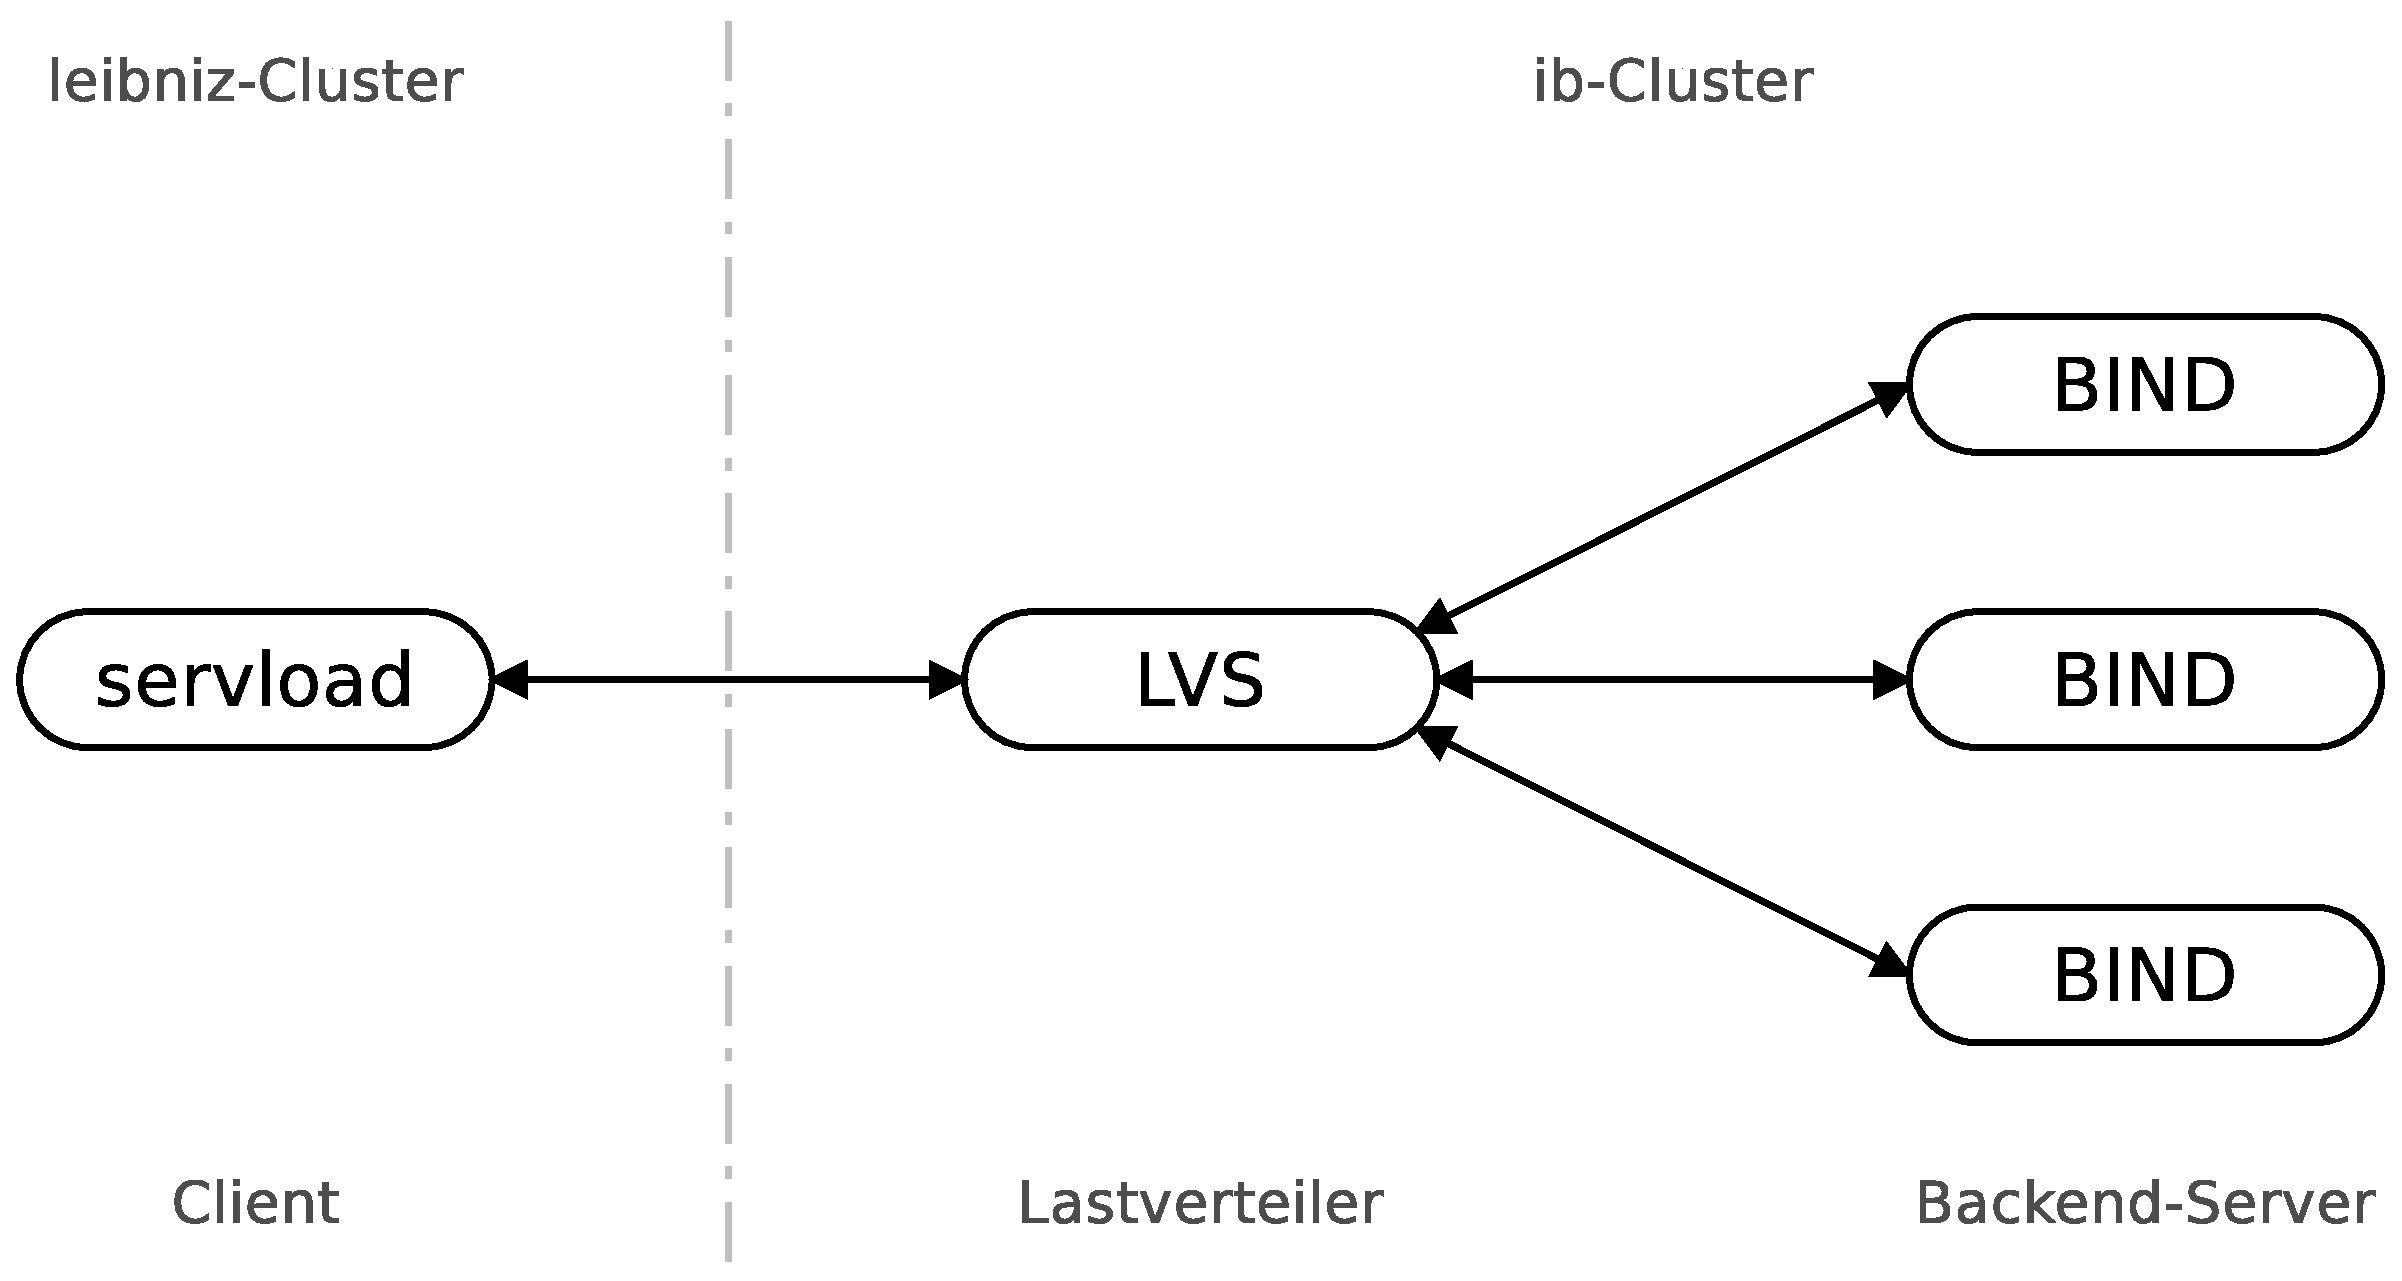
\includegraphics[width=12cm]{images/test-system}
			\caption{Aufbau des Messsystems}
			\label{fig:messsystem}
		\end{figure}

		\section{System} % {{{
		\label{sec:system}

		Der Fokus der Messung liegt auf der Lastverteilung. Die Lastverteilung kann entweder nur vom
		Lastverteiler aus gesteuert werden, oder, wie im \textit{salbnet}-Fall, mit Hilfe zusätzlicher
		Informationen von den Backend-Servern beeinflusst werden. Das Messsystem soll ein DNS-Cluster,
		wie es bei Root-Servern, TLDs oder große SLDs vorkommt, simulieren.  Es besteht aus einem
		Client, welcher über ein Netzwerk mit einem Lastverteiler verbunden ist. Dieser ist wiederum
		über ein anderes Netzwerk mit 3 heterogenen Backend-Servern verbunden. Der Aufbau ist in
		Abbildung \ref{fig:messsystem} grafisch dargestellt. Der Client ist ein Rechner im
		leibniz-Cluster, auf dem der servload Benchmark \cite{menski2012} ausgeführt wird. In dem
		Zielnetzwerk des ib-Clusters kommt auf dem Lastverteiler LVS zum Einsatz. Alle 3 heterogenen
		Backend-Server stellen einen BIND DNS-Server bereit. Die genauen technischen Daten der Server
		und die Versionen der verwendeten Software sind in Anhang \ref{cha:messumgebung} aufgeführt.
		Das System bietet ausschließlich den DNS-Dienst durch die Backend-Server an. Dabei werden nur
		DNS-Anfragen über UDP unterstützt. Die möglichen Resultate einer DNS-Anfrage an das System sind
		eine Antwort oder keine Antwort. Um verschiedene Messungen zu vergleichen, werden die folgenden
		Metriken genutzt:

		\begin{itemize}
			\item Verbindungszeit in Millisekunden
			\item Antwortzeit in Millisekunden
			\item Anzahl der nicht beantworteten Anfragen (Timeout: eine Sekunde)
			\item CPU-Auslastung der Backend-Server in Prozent
		\end{itemize}

		% section System }}}

		\section{Experiment} % {{{
		\label{sec:experiment}

			Um die Experimente festzulegen, müssen alle Parameter ermittelt werden, welche die Leistung
			des Systems beeinflussen. Bei diesen Messungen sind die folgenden Eigenschaften entscheidend:

			\begin{itemize}
				\item Systemparameter (statisch)
					\begin{itemize}
						\item Geschwindigkeit des Netzwerks
						\item Leistung der CPU
						\item Größe des Arbeitsspeichers
						\item Performanz des Lastverteilers
						\item Performanz des DNS-Servers
						\item Netzwerk-Stack des Betriebssystems
						\item Andere Last auf dem Netzwerk
						\item Andere Last auf den Servern
					\end{itemize}
				\item[]
				\item Lastparameter (variabel)
					\begin{itemize}
						\item Größe der DNS-Zone
						\item Art des DNS-Servers (iterativ oder rekursiv)
						\item Lastverteilungsalgorithmus
						\item Anzahl der DNS-Anfragen
						\item Anzahl der DNS-Anfragen pro Sekunde
					\end{itemize}
			\end{itemize}

			Von den Lastparameter sind die Größe der DNS-Zone und die Art des DNS-Servers statisch. Als
			DNS-Zone wird die \texttt{haiti.cs.uni-potsdam.de}-Zone mit dem Stand vom 26.  Oktober 2011
			genutzt. Die BIND Server werden alle als iterative Nameserver betrieben, dass heißt, Anfragen
			außerhalb der \texttt{haiti.cs.uni-potsdam.de} werden mit einem Verweis auf die Root-Server
			beantwortet. Dies ist realistisch, da Nameserver der Root-Zone oder TLDs auch iterative
			Nameserver nutzen, und \textit{salbnet} vor allem für dieses Einsatzgebiete konzipiert ist.

			Die Faktoren, welche während den Messungen variiert werden, sind der
			Lastverteilungsalgorithmus, die Anzahl der DNS-Anfragen und die Anzahl der DNS-Anfragen pro
			Sekunde. Als Lastverteilungsalgorithmus wird der Standard-Weighted-Round-Robin-Algorithmus
			(\textit{wrr}) des LVS verwendet und \textit{salbnet} mit der Dynamic Pressure Relive Meldestrategie. Als Gewichte
			für den Weighted-Round-Robin-Algorithmus wurden die Werte 788, 623 und 1180 für die Nodes ib4,
			ib6 und ib8 verwendet. Diese Werte wurden mit dem UnixBench-Benchmark \cite{unixbench}
			ermittelt. Die vollständigen Ergebnisse sind im Anhang \ref{cha:unixbench} aufgelistet. Für
			die DNS-Anfragen wurde ein anonymisiertes Log des Nameservers der
			\texttt{haiti.cs.uni-potsdam.de}-Domain genutzt. Das Log enthält den Zeitraum vom 27.
			September 2011 10:41 bis zum 2. Oktober 2011 6:25. Es wurden 1026 Sessions, dabei umfasst eine
			Session alle Anfragen eines Users (IP-Adresse), und 1.003.149 DNS-Anfragen\footnote{Weitere
			Statistiken zur \texttt{haiti.cs.uni-potsdam.de}-Zone und dem DNS-Log sind in Anhang
			\ref{cha:haiti} zu finden.} registriert. Im Durchschnitt werden 2,41 Anfragen pro Sekunde
			gestellt. Das heißt, würde das Log unverändert eingesetzt werden, wäre keine Überlastsituation
			auf einem DNS-Cluster mit 3 Backend-Servern zu erwarten. Daher wurde ein 5 Minuten langer
			Ausschnitt aus dem Log verwendet.  Der Verlauf der Anfragen pro Sekunde ist in Abbildung
			\ref{fig:requests} zu sehen. Um 3 verschiedene Lastsituationen zu erzeugen, wurde das Log
			dann vor dem Testen mit Hilfe von servload \cite{menski2012} verstärkt, und jede
			Anfrage um einen bestimmten Faktor vervielfacht. Es wurden die Faktoren 400, 800 und 1600
			gewählt. Die entsprechenden Kennzahlen dieser Faktoren sind in Tabelle \ref{tab:multiply}
			aufgeführt. Der Messplan mit der Anzahl der Durchläufe ist in Tabelle \ref{tab:messplan} zu
			sehen.


			\begin{figure}
				\centering
				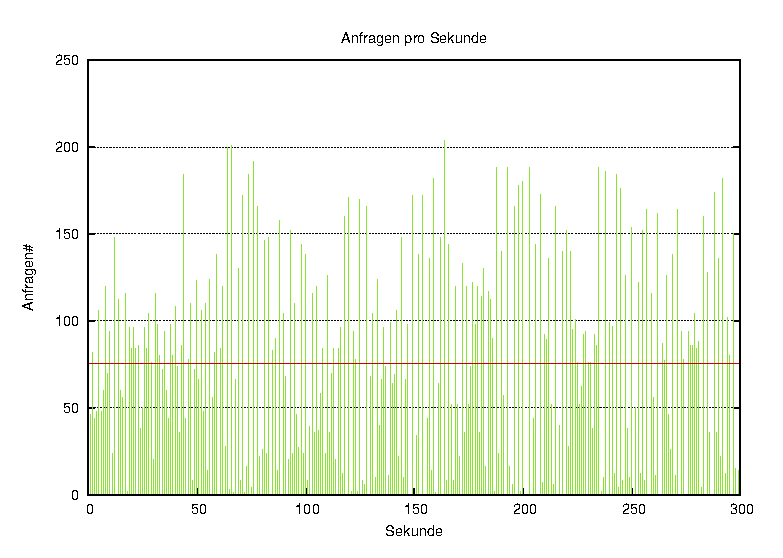
\includegraphics[width=\textwidth]{plots/requests}
				\caption{Anfragen pro Sekunde für das Log vom 29. September 2011 von 5:55 bis 6:00}
				\label{fig:requests}
			\end{figure}

			\begin{table}
				\centering
				\begin{tabular}{|lrrrr|}\hline
					Faktor & Anfragen & Sessions & $\varnothing$ \nicefrac{Anfragen}{Sekunde} &
					max. \nicefrac{Anfragen}{Sekunde} \\\hline\hline
					1 & 22.594 & 33 & 75,31 & 204 \\
					400 & 9.037.600 & 13.200 & 30.125,33 & 81.600 \\
					800 & 18.075.200 & 26.400 & 60.250,67 & 163.200 \\
					1600 & 36.150.400 & 52.800 & 120.501,33 & 326.400 \\\hline
				\end{tabular}
				\caption{Kennzahlen des modifizierten Log-Intervalls}
				\label{tab:multiply}
			\end{table}

			\begin{table}
				\centering
				\begin{tabular}{|r|c|c|c||c|}\hline
					& 400 & 800 & 1600 & Summe \\\hline
					\textit{wrr} & 51 & 51 & 51 & 153 \\
					\textit{salbnet} & 51 & 51 & 51 & 153 \\
												 & & & & 306 \\\hline
				\end{tabular}
				\caption{Anzahl der Messungen je Kombination aus Lastverteilungsalgorithmus und Faktor}
				\label{tab:messplan}
			\end{table}

		% section Experiment }}}

		\section{Ergebnisse} % {{{
		\label{sec:Ergebnisse}

			Zur Auswertung der Messungen wurden die Ausgaben des servload-Benchmarks verwendet. Außerdem
			wurden die Load und die Auslastung der CPU und des Arbeitsspeichers der Backend-Server
			minütlich mit Hilfe eines Skriptes über \texttt{net-snmp} abgefragt. Grundlegend ist
			festzuhalten, dass die Erweiterung von \textit{salbnet} für UDP-Anfragen funktioniert. Während der
			Tests kam es zu keinen Ausfällen oder auffälligem Verhalten. Danach wurden die beiden
			Lastverteilungsverfahren \textit{wrr} und \textit{salbnet} unter den Metriken aus Abschnitt \ref{sec:system}
			verglichen. Die Bewertung geschieht dabei nach den folgenden Kriterien:

			\begin{itemize}
				\item Vermeiden von verlorenen Anfragen
				\item Minimale Antwortzeiten
				\item Minimale Verbindungszeiten
				\item Konstante CPU-Auslastung
				\item Gleichmäßige CPU-Auslastung aller Backend-Server
			\end{itemize}

			Die CPU-Auslastungen für die Nodes im ib-Cluster sind für den \textit{wrr}-Algorithmus in Abbildung
			\ref{fig:cpu-wrr}, und für \textit{salbnet} in Abbildung \ref{fig:cpu-salbnet} zu sehen. Es ist zu
			erkennen, dass die CPU-Auslastung bei \textit{salbnet} wesentlich konstanter ist als bei \textit{wrr}.
			Allerdings liegt sie bei der ib6 für alle Faktoren mit \textit{salbnet} immer nahe \unit[100]{\%}. Dies könnte
			auf eine ungleichmäßige Verteilung hindeuten. Hingegen liegen die Werte der ib4 und ib8 sehr
			dicht beieinander. Die Anzahl der verlorenen Anfragen (siehe Tabelle \ref{tab:timeout} und
			Abbildung \ref{fig:ergebnis}) ist bei \textit{salbnet} immer geringer als bei \textit{wrr}.  Die verlorenen
			Anfragen von \textit{salbnet} entsprechen für den Faktor 400 ca. \unit[25]{\%}, für 800 ca. \unit[33]{\%} und für 1600
			ca. \unit[50]{\%} der verlorenen Anfragen von \textit{wrr}. Noch deutlicher werden die Unterschiede bei dem
			Vergleich der
			Antwortzeiten (siehe Tabelle \ref{tab:response} und Abbildung \ref{fig:ergebnis}) und der
			Verbindungszeiten  (siehe Tabelle \ref{tab:connect} und Abbildung \ref{fig:ergebnis}).
			So entspricht die Antwortzeit von \textit{salbnet} nur ca. \unit[15]{\%} der von \textit{wrr} und die Verbindungszeit im
			Durchschnitt nur ca. \unit[30]{\%}.

			\begin{figure}
				\centering
				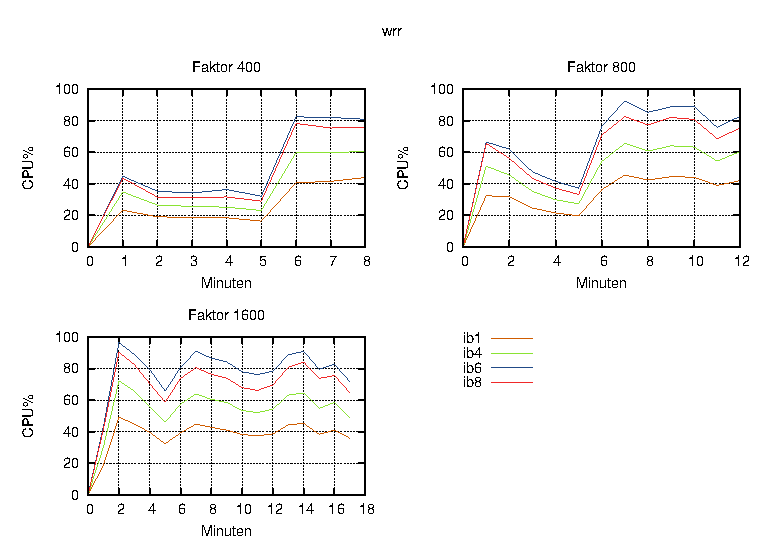
\includegraphics[width=14cm]{plots/cpu-wrr}
				\caption{CPU Auslastung der Nodes ib1, ib4, ib6 und ib8 mit \textit{wrr} als
				Lastverteilungsalgorithmus}
				\label{fig:cpu-wrr}
			\end{figure}

			\begin{figure}
				\centering
				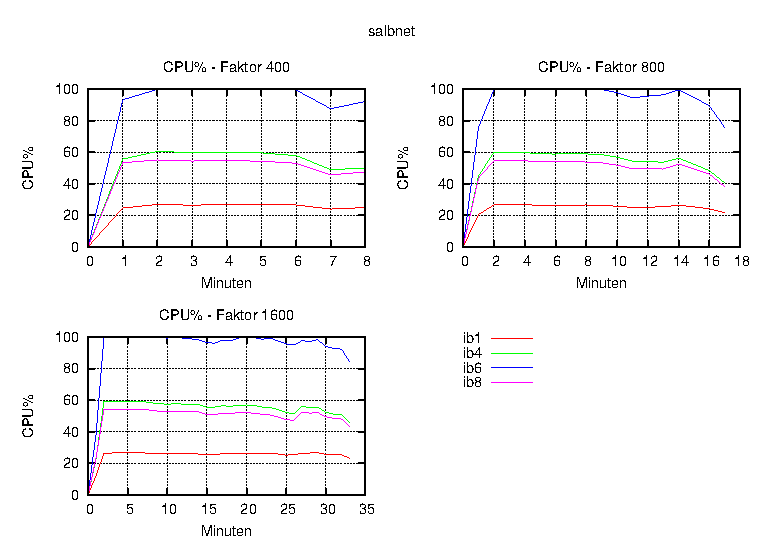
\includegraphics[width=14cm]{plots/cpu-salbnet}
				\caption{CPU Auslastung der Nodes ib1, ib4, ib6 und ib8 mit \textit{salbnet} als
				Lastverteilungsalgorithmus}
				\label{fig:cpu-salbnet}
			\end{figure}

			\begin{figure}
				\centering
				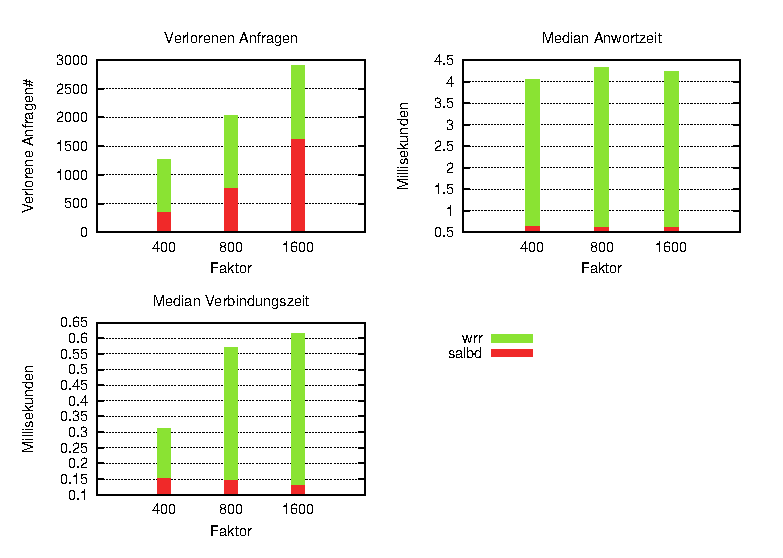
\includegraphics[width=13cm]{plots/servload}
				\caption{Vergleich von \textit{wrr} und \textit{salbnet} für die Metriken: Verlorene Anfragen, Antwortzeit und Verbindungszeit}
				\label{fig:ergebnis}
			\end{figure}

			\begin{table}
				\centering
				\begin{tabular}{|r|c|c|}\hline
					Faktor & \textit{wrr} & \textit{salbnet} \\\hline\hline
					400 & 1273,39 (182.727,4/427,5) & 343,16 (10.444,9/102,2)\\
					800 & 2038,53 (395.551,1/628,9) & 759,86 (30.414,0/174,4)\\
					1600 & 2910,16 (386.854,5/622,0) & 1612,78 (55.845,1/236,3)\\\hline
				\end{tabular}
				\caption{Anzahl der verlorenen Anfragen (Varianz/Standardabweichung)}
				\label{tab:timeout}
			\end{table}

			\begin{table}
				\centering
				\begin{tabular}{|r|c|c|}\hline
					Faktor & \textit{wrr} & \textit{salbnet} \\\hline\hline
					400 & 4,05 (0,95/0,98) & 0,64 (0,00/0,01)\\
					800 & 4,33 (2,50/1,58) & 0,61 (0,00/0,01)\\
					1600 & 4,24 (2,17/1,47) & 0,60 (0,00/0,02)\\\hline
				\end{tabular}
				\caption{Median Antwortzeit in Millisekunden (Varianz/Standardabweichung)}
				\label{tab:response}
			\end{table}

			\begin{table}
				\centering
				\begin{tabular}{|r|c|c|}\hline
					Faktor & \textit{wrr} & \textit{salbnet} \\\hline\hline
					400 & 0,31 (0,00/0,05) & 0,15 (0,00/0,00)\\
					800 & 0,57 (0,05/0,22) & 0,14 (0,00/0,01)\\
					1600 & 0,61 (0,10/0,31) & 0,13 (0,00/0,00)\\\hline
				\end{tabular}
				\caption{Median Verbindungszeit in Millisekunden (Varianz/Standardabweichung)}
				\label{tab:connect}
			\end{table}

		% section Ergebnisse }}}

		\section{Fazit} % {{{
		\label{sec:Fazit}

		Als Fazit der Messungen ist zu sagen, dass die Erweiterung von \textit{salbnet} für UDP-Pakete
		erfolgreich umgesetzt wurde. Die Implementation funktioniert und hat in den Tests eine hohe
		Leistungsfähigkeit bewiesen. In allen verglichenen Metriken ist \textit{salbnet} dem \textit{wrr}-Algorithmus
		überlegen. Nur die CPU-Auslastung der ib6 war im Vergleich zu den anderen Backend-Servern zu
		hoch. Dies kann an zu optimistischen oder zu späten Credit-Meldungen liegen. Zusammenfassend
		kann gesagt werden, dass das Konzept und die Implementierung höchstwahrscheinlich noch
		Verbesserungspotenzial bieten, die aktuelle Version jedoch bereits den Vorteil von
		selbst-adaptiver Lastverteilung auch für UDP-Verkehr verdeutlicht.

		% section Fazit }}}

	% chapter Messungen }}}

	\chapter{Zusammenfassung und Ausblick} % {{{
	\label{cha:zusammenfassung}

	Dieses letzte Kapitel gibt in Abschnitt \ref{sec:zusammenfassung} eine abschließende
	Zusammenfassung der erreichten Ziele und bewertet sie. In Abschnitt \ref{sec:ausblick} wird ein
	Ausblick auf mögliche Verbesserungen und Weiterentwicklungen gegeben.

		\section{Zusammenfassung} % {{{
		\label{sec:zusammenfassung}

		Das Ziel der Arbeit war es, das bestehende selbst-adaptive Lastverteilungssystem \textit{salbnet} so zu
		erweitern, dass auch UDP-Anwendungen unterstützt werden. Dazu wurde als Anwendungsfall der Betrieb
		eines DNS-Clusters gewählt, weil DNS-Verkehr hauptsächlich aus UDP-Anfragen besteht. Weiterhin hat
		das DNS durch seinen Aufbau als baumartige Struktur kritische Bereiche, die eine Lastverteilung
		zwingend notwendig machen. So werden vor allem bei DNS-Root-Servern und Nameservern von
		TLDs DNS-Cluster genutzt, um hohe Anfrageaufkommen abzufangen, und erfolgreich zu beantworten. Der
		Einsatz von \textit{salbnet} im DNS ist klar in den oberen Ebenen des DNS-Baumes angeordnet, da bei
		kleineren Domains andere einfachere Lastverteilungsmechanismen verwendet werden.

		Um \textit{salbnet} auch für UDP-Anfragen nutzen zu können, musste eine repräsentative Metrik für die
		Auslastung des Nameservers gefunden werden. Dabei war vor allem wichtig, dass aus dieser Metrik
		eine Credit-Berechnung erfolgen kann. Dies stellte das hauptsächliche Problem dar, zumal nicht jede
		Lastmetrik dazu geeignet ist, die noch möglichen Verbindungen zu bestimmen. So kann an vielen
		Faktoren erkannt werden, wann ein Server in einer Überlastsituation ist. Jedoch ist die
		Abschätzung der noch möglichen Anfragen, bevor es zu einer Überlastsituation kommt, nicht
		trivial. Dabei hat sich ein ähnlicher Ansatz herausgebildet, wie beim bereits implementierten
		TCP-Anwendungsfall. Durch das Überwachen des aktuell freien Speicherplatzes in der Receive-Queue
		des UDP-Sockets, kann mit Hilfe einer Abschätzung über die durchschnittliche Paketgröße die
		Credit-Berechnung erfolgreich durchgeführt werden.

		Dieses Vorgehen zur Berechnung der Credits wurde anschließend in \textit{salbnet} implementiert. Dabei
		kam es zu keinen größeren Problemen und das vorher entwickelte Konzept konnte direkt umgesetzt
		werden. Da bei der Konzipierung von \textit{salbnet} bereits der UDP-Fall bedacht wurde, mussten keine
		größeren Änderungen an der Struktur vorgenommen werden. Größtenteils waren bereits alle
		Erweiterungspunkte gut eingepflegt und mussten nur ausprogrammiert werden.

		Nach der erfolgreichen Implementation wurden mehrere Messungen durchgeführt. Sie hatten zum
		Ziel, die Funktionstüchtigkeit der Erweiterung von \textit{salbnet} zu beweisen. Ein Vergleich mit
		einem Standardalgorithmus sollte eine Einschätzung der Leistungsfähigkeit der neuen UDP-Metrik
		geben.  Die Ergebnisse bestätigten sowohl die volle Funktionsfähigkeit der Erweiterung, als auch
		die Konkurrenzfähigkeit gegenüber Standardalgorithmen der Lastverteilung. Das Ergebnis fiel klar
		zu Gunsten von \textit{salbnet} aus, und bestätigte die Behauptung, dass sich die selbst-adaptive
		gegen die statische Lastverteilung behauptet.

		% section Zusammenfassung }}}

		\section{Ausblick} % {{{
		\label{sec:ausblick}

		Abschließend kann festgehalten werden, dass die entwickelte und implementierte Metrik
		funktioniert. Allerdings wurde bei den Tests eine sehr hohe CPU-Auslastung für den schwächsten
		Server festgestellt. Dies zeigt, dass die Metrik weiter verfeinert werden sollte. Dabei ist die
		Frage, ob die Abschätzung des verfügbaren Speicherplatzes in der Receive-Queue zu optimistisch war.
		So könnte man zum Beispiel nicht vom Median der letzten DNS-Pakete ausgehen, sondern den Maximalwert nutzen.
		Dies würde eine pessimistischere Abschätzung erzeugen, dafür aber vielleicht eher
		Überlastsitutationen verhindern.

		Ein anderer Diskussionspunkt ist die Phase zwischen zwei Credit-Meldungen. Bis jetzt wird diese
		Phase ignoriert und nur die Anzahl an verworfenen Verbindungen als Abschätzung dafür genutzt, ob
		zwischenzeitlich eine Überlastsitutation existierte. Es wäre jedoch auch möglich, stetig
		Messwerte zu sammeln, und daraus eine Tendenz zu ermitteln. Diese würde eine bessere Vorhersage
		ermöglichen, allerdings auch einen höheren Aufwand bedeuten.

		Weiterhin bleibt das Problem des realen Speicherplatzes eines DNS-Pakets in der Receive-Queue.
		Die hier verwendete experimentell ermittelte Abschätzung ist stark abhängig von der
		Kernel-Version und sollte unabhängig von dieser umgesetzt werden. Sollte \textit{salbnet} für neuere
		Kernel-Versionen portiert werden, könnte allgemein die UDP-Erweiterung durch aktuellere Techniken
		verbessert werden. Einige davon wurden bereits in Abschnitt \ref{sec:anforderungen} erwähnt.

		% section Ausblick }}}

	% chapter Zusammenfassung }}}

	% Mainmatter }}}

	% Appendix {{{
	\appendix

	\chapter{Messumgebung} % {{{
	\label{cha:messumgebung}

	Dieser Anhang liefert Informationen bezüglich der für die Messungen verwendeten Systeme (siehe
	Abschnitt \ref{sec:Systeme}),
	der genutzten Softwareversionen (siehe Abschnitt \ref{sec:software}) und Konfigurationen
	(siehe Abschnitt \ref{sec:konfigurationen}).

		\section{Systeme} % {{{
		\label{sec:Systeme}

			In diesem Abschnitt werden die technischen Daten der Systeme vorgestellt, welche in der
			Messumgebung verwendetet wurden.

		\begin{description}
			\item[Rolle:] Client
					\begin{description}
						\item[Cluster:] leibniz
						\item[Hostname:] node015
						\item[CPU:] Intel Xeon E5520 @ \unit[2,27]{GHz} (Quad-Core)
						\item[RAM:] \unit[12]{GB}
					\end{description}
			\item[Rolle:] Lastverteiler
					\begin{description}
						\item[Cluster:] ib
						\item[Hostname:] ib1
						\item[CPU:] 2 $\times$ AMD Opteron 244 @ \unit[1,8]{GHz} (Single-Core)
						\item[RAM:] \unit[4]{GB}
					\end{description}
			\item[Rolle:] Backend-Server 1
					\begin{description}
						\item[Cluster:] ib
						\item[Hostname:] ib4
						\item[CPU:] 2 $\times$ AMD Opteron 244 @ \unit[1,8]{GHz} (Single-Core)
						\item[RAM:] \unit[4]{GB}
					\end{description}
			\item[Rolle:] Backend-Server 2
					\begin{description}
						\item[Cluster:] ib
						\item[Hostname:] ib6
						\item[CPU:] Intel Pentium @ \unit[2,8]{GHz} (Single-Core)
						\item[RAM:] \unit[4]{GB}
					\end{description}
			\item[Rolle:] Backend-Server 3
					\begin{description}
						\item[Cluster:] ib
						\item[Hostname:] ib8
						\item[CPU:] Intel Xeon 3040 @ \unit[1,86]{GHz} (Dual-Core)
						\item[RAM:] \unit[4]{GB}
					\end{description}
		\end{description}

		% section Systeme }}}

		\section{Software} % {{{
		\label{sec:software}

		In diesem Abschnitt wird die zur Messung genutzte Software mit ihren entsprechenden Versionen,
		und gegebenenfalls der Subversion-Revision, aufgelistet.

		\begin{description}
			\item[Betriebssystem:] Debian
				\begin{description}
					\item[Version:] 5.0.9 (Lenny)
					\item[Kernel:] 2.6.26-2-amd64
					\item[Nodes:] node015
					\item[rmem\_default:] \unit[124928]{Byte}
					\item[rmem\_max:] \unit[16777216]{Byte}
				\end{description}
			\item[Betriebssystem:] CentOS
				\begin{description}
					\item[Version:] 5.7 (Final)
					\item[Kernel:] 2.6.18-274.12.1.el5
					\item[Nodes:] ib1, ib4, ib6, ib8
					\item[rmem\_default:] \unit[25165824]{Byte}
					\item[rmem\_max:] \unit[25165824]{Byte}
				\end{description}
			\item[DNS-Server:] BIND
				\begin{description}
					\item[Version:] 9.3.6
					\item[Release:] 20.P1.el5\_8.1
				\end{description}
			\item[Benchmark:] servload
				\begin{description}
					\item[Version:] 0.5.1-dns
					\item[Revision:] 2026
				\end{description}
			\item[salbnet:] salbd
				\begin{description}
					\item[Version:] 0.4.5
					\item[Revision:] 2028
				\end{description}
			\item[salbnet:] libnethook
				\begin{description}
					\item[Version:] 0.2
					\item[Revision:] 2027
				\end{description}
			\item[salbnet:] libnetmsg
				\begin{description}
					\item[Version:] 0.4.4
					\item[Revision:] 1980
				\end{description}
		\end{description}

		% section Software }}}

		\section{Konfigurationen} % {{{
		\label{sec:konfigurationen}

			Die verwendeten Konfigurationen für \textit{salbd} und BIND sind in diesem Abschnitt als Anhang
			dargestellt.

			\lstinputlisting[language=sh,caption={\textit{salbd} Konfiguration für ib1 (LVS)},label=lst:salbd-server]{listings/salbd.conf.server}

		\lstinputlisting[language=sh,caption={\textit{salbd} Konfiguration für ib4, ib6 und ib8 (BIND)},label=lst:salbd-client]{listings/salbd.conf.client}

		\lstinputlisting[language=sh,caption={\textit{salbd} BIND Konfiguration für ib4, ib6 und ib8},label=lst:salbd-bind]{listings/salbd.networks.conf.client}

		\lstinputlisting[language=sh,caption={BIND Konfiguration für ib4, ib6 und ib8},label=lst:bind-conf]{listings/named.conf}

		% section Konfigurationen }}}

	% chapter Messumgebung }}}

	\chapter{UnixBench} % {{{
	\label{cha:unixbench}

			In diesem Anhang wird das Ergebnis des UnixBench-Benchmark für die Nodes ib4, ib6 und
			ib8 aufgelistet.

	\lstinputlisting[lastline=77,language=,breaklines=true,numbers=none,caption={UnixBench Resultat für die Node ib4}]{listings/result_unixbench.dat}
	\lstinputlisting[firstline=83,lastline=124,language=,breaklines=true,numbers=none,caption={UnixBench Resultat für die Node ib6}]{listings/result_unixbench.dat}
	\lstinputlisting[firstline=130,language=,breaklines=true,numbers=none,caption={UnixBench Resultat für die Node ib8}]{listings/result_unixbench.dat}

	% chapter UnixBench }}}

	\chapter{Haiti-Zone} % {{{
	\label{cha:haiti}

	  In diesem Anhang sind Statistiken zur \texttt{haiti.cs.uni-potsdam.de}-Zone und dem verwendeten
		Log dargestellt.

		\begin{table}[h]
			\centering
			\begin{tabular}{|c|c|}\hline
				Resource Record & Anzahl \\\hline\hline
				A & 107 \\
				NS & 4 \\
				MX & 2 \\
				CNAME & 2 \\
				PTR & 106 \\
				SOA & 1 \\\hline
			\end{tabular}
			\caption{Anzahl der DNS-Typen in der \texttt{haiti.cs.uni-potsdam.de}-Zone mit dem Stand vom 26. Oktober 2011}
			\label{tab:rr-domain}
		\end{table}

		\begin{table}[h]
			\centering
			\begin{tabular}{|c|rr|}\hline
				Start & 27. September 2011 & 10:41 \\
				Ende & 2. Oktober 2011 & 6:25 \\
				Anfragen & 1003149 & \\
				Sessions & 1026 & \\
				Anfragen je Sekunde & 2,41 &\\
				Anfragen je Session & 977,73 &\\ \hline
			\end{tabular}
			\caption{Analyse des BIND Logs des \texttt{haiti.cs.uni-potsdam.de}-Nameserves}
			\label{tab:log}
		\end{table}


		\begin{table}
			\centering
			\begin{tabular}{|c|rr|}\hline
				AAAA & 609821 & \unit[60,791]{\%}\\
				A & 327861 & \unit[32,683]{\%}\\
				PTR & 60553 & \unit[6,036]{\%} \\
				NS & 3575 & \unit[0,356]{\%}\\
				MX & 669 & \unit[0,067]{\%}\\
				SOA& 355 & \unit[0,035]{\%} \\
				TXT& 237 & \unit[0,024]{\%} \\
				ANY& 36 & \unit[0,004]{\%} \\
				SRV& 26 & \unit[0,003]{\%} \\
				A6& 14 & \unit[0,001]{\%} \\
				HINFO& 1 & \unit[0,000]{\%} \\
				AXFR& 1 & \unit[0,000]{\%} \\\hline
			\end{tabular}
			\caption{Anzahl der DNS-Typen im BIND Log des \texttt{haiti.cs.uni-potsdam.de}-Nameserves}
			\label{tab:log}
		\end{table}

	% chapter Haiti-Zone }}}

	\chapter{sk\_buff} % {{{
	\label{cha:skbuff}

	\lstinputlisting[firstline=193,lastline=304,caption={\texttt{sk\_buff}-Datenstruktur in der Datei
	\texttt{skbuff.h} vom Linux-Kernel 2.6.18},label=lst:skbuff]{listings/skbuff.h}

	% chapter skbuff }}}

	% Appendix }}}

	% Backmatter {{{
	\backmatter
	\pagenumbering{Roman}

	\listoffigures{}
	\listoftables{}

	% Bibliography {{{
	% \nocite{*}
	\bibliographystyle{dinat}
	\bibliography{references}
	% }}}

	% Backmatter }}}

\end{document}
